\documentclass[12pt,a4paper,twoside]{book}

\usepackage[utf8]{inputenc}

% general usepackage stuff
\usepackage{times}
\usepackage{mathptmx}
\usepackage{booktabs}
\usepackage{graphicx}
\usepackage{titlesec}
\usepackage{amssymb}
\usepackage{color}

% additional packages
\usepackage{rotating} 	                 % sidesways figures
\usepackage[font=scriptsize]{subcaption} % subfigures

% table alignment
\usepackage{multirow}
\usepackage{makecell}

% aligned minipages(p) for tables
\newcolumntype{L}[1]{>{\raggedright\arraybackslash}p{#1}} % left aligned
\newcolumntype{C}[1]{>{\centering\arraybackslash}p{#1}}   % center aligned
\newcolumntype{R}[1]{>{\raggedleft\arraybackslash}p{#1}}  % right aligned

%% labels and page stuff
\renewcommand{\labelitemi}{$\diamond$}
\renewcommand{\labelitemii}{$\circ$}

\setcounter{secnumdepth}{3}

%\setlength{\oddsidemargin}{-0.5cm}
%\setlength{\evensidemargin}{-0.5cm}

\setlength{\oddsidemargin}{4.58mm}%final
\setlength{\evensidemargin}{-4.92mm}%final


\setlength{\textwidth}{15.95cm}%final
\setlength{\textheight}{23.5cm}
\setlength{\voffset}{-1.45cm} %


%% todo
\newcommand{\todo}[1]{\textcolor{red}{[todo: }#1\textcolor{red}{]}}
\newcommand{\todoh}[1]{} 
\newcommand{\done}[1]{} 

%% smallerText
\newcommand{\smallerTextSize}{10}
\newcommand{\smallerTextSkip}{12}
\newcommand{\smallerBegin}{\fontsize{\smallerTextSize}{\smallerTextSkip}\selectfont}
\newcommand{\smallerEnd}{\normalsize}
\newcommand{\smaller}[1]{\smallerBegin #1\smallerEnd}

%%reference to defintion
\newcommand{\defref}[1]{\ref{#1} on page \pageref{#1}}

%% special, short for shell
\newcommand{\shl}[1]{\sf \small #1\rm\normalsize}

%% indentation in tables
\newcommand{\tabind}[1]{\rule{#1mm}{0cm}}

%% smaller in captions
\newcommand{\captionfonts}{\smallerBegin}
                                                                                                                                                                              
\makeatletter  % Allow the use of @ in command names
\long\def\@makecaption#1#2{%
  \vskip\abovecaptionskip
  \sbox\@tempboxa{{\captionfonts #1: #2}}%
  \ifdim \wd\@tempboxa >\hsize
    {\captionfonts #1: #2\par}
  \else
    \hbox to\hsize{\hfil\box\@tempboxa\hfil}%
  \fi
  \vskip\belowcaptionskip}
\makeatother   % Cancel the effect of \makeatletter

%% clear page before new chapter
\makeatletter
\def\cleardoublepage{\clearpage\if@twoside \ifodd\c@page\else
\hbox{}
\vspace*{\fill}
\begin{center}
% This page intentionally contains only this sentence.
\end{center}
\vspace{\fill}
\thispagestyle{empty}
\newpage
\if@twocolumn\hbox{}\newpage\fi\fi\fi}
\makeatother

%% abbreviations
\usepackage{nomencl}
\let\abbrev\nomenclature
\renewcommand{\nomname}{List of Abbreviations}
\setlength{\nomlabelwidth}{.25\hsize}
\renewcommand{\nomlabel}[1]{#1 \dotfill}
\setlength{\nomitemsep}{-\parsep}
\makenomenclature
\newcommand{\Listofabbrev}{
\printnomenclature
\newpage
}

%% chapter title formatting
\titleformat{\chapter}[display]{ \raggedleft }{\fontsize{52}{63}\selectfont \bf \thechapter }{0.2cm}{\fontsize{32}{38.7}\selectfont  }[]

%% header formatting
\renewcommand{\chaptermark}[1]{%
\markboth{\chaptername
\ \thechapter.\ #1}{}}
\renewcommand{\sectionmark}[1]{\markright{\thesection.\ #1}}
\usepackage{fancyhdr}
\pagestyle{fancy}
\fancyhf[LEH,ROH]{\thepage}
\fancyhf[REH]{\smaller{\nouppercase{\leftmark}}}
\fancyhf[LOH]{\smaller{\it \nouppercase{\rightmark}}}
\fancyhf[COF]{\rule{0.2cm}{0.0cm}}
\fancyhf[CEF]{\rule{0.2cm}{0.0cm}}
\renewcommand{\headrulewidth}{0pt}

%% macro for figures
%\usepackage{svg}
\usepackage{amsmath}
%\newcommand{\printlabel}{}
%\newcommand{\abcdef}[1]{\tiny #1 \normalsize}

		%% arguments: graphics file, label, caption, smallcaption
\newcommand{\insertFigure}[4]{\begin{figure}[top] \smallerBegin \centering \includegraphics{#1}  \\  \caption{\label{#2}\smallerBegin #3 \footnotesize{#4}  \smallerEnd }  
\end{figure}	}
%% macro for figures with short caption
		%% arguments: graphics file, label, caption, smallcaption, shortcaption
\newcommand{\insertFigureShort}[5]{\begin{figure}[top] \smallerBegin \centering \includegraphics{#1} \label{#2} \\ \caption[#5]{\smallerBegin #3 \footnotesize{#4} \smallerEnd } 
\end{figure}	}
%\renewcommand{\topfraction}{1}

\newcommand{\spaceafterpar}{\vspace{14.48pt}}

\renewcommand{\floatpagefraction}{.75} % vorher: .5
\renewcommand{\textfraction}{.1}       % vorher: .2
\renewcommand{\topfraction}{.8}        % vorher: .7
\renewcommand{\bottomfraction}{.5} 
\setcounter{topnumber}{3}              % vorher: 2
\setcounter{bottomnumber}{2}           % vorher: 1
\setcounter{totalnumber}{5}            % vorher: 3
% from: http://www.matthiaspospiech.de/latex/vorlagen/allgemein/preambel/9/

% macros for tables
    %% arguments: columns
\newcommand{\tableBegin}[1]{\begin{table}[top] \begin{center} \smallerBegin \begin{tabular}{#1}}
		%% arguemtns: caption, label
\newcommand{\tableEnd}[2]{ \end{tabular} \smallerEnd \end{center} \caption{#1} \label{#2}	\end{table}}

%% shortcuts
\newcommand{\emit}[1]{\item \emph{#1}:}
\newcommand{\firstappear}[2]{\emph{#1} (#2) \abbrev{#2}{#1}}

\hyphenation{or-gan-izing}

%% definitions

\newtheorem{definition}{Definition}

%% examples
\newcommand{\exampleBeginText}[1]{\paragraph{#1}}
\newcommand{\exampleEnd}{\vspace{6mm}}
\newcommand{\exampleBegin}{\exampleBeginText{Example}}

% algorithms
\usepackage[english,ruled,vlined, slide, norelsize]{algorithm2e}

% ref imgs
\usepackage{hyperref}

% references
\usepackage{cleveref}
\usepackage[numbers,sort]{natbib}
\setlength{\bibsep}{0.0pt}
\bibliographystyle{plainnat}

\usepackage{csvsimple}

% math operators
\DeclareMathOperator*{\argmax}{\arg\!\max}
\DeclareMathOperator*{\argmin}{\arg\!\min}


% Front Matter

\newcommand{\titleLineOne}{Anomaly Detection through}
\newcommand{\titleLineTwo}{Video Generation Forecasting}
\newcommand{\titleLineThree}{}
\newcommand{\documentdate}{\today}
\newcommand{\studentname}{Fabian Sebastian Hofmann}
\newcommand{\abstracttextde}{In den letzten zwei Jahrzehnten hat sich die Menge an Videodaten, die von immer mehr und immer kostengünstigeren Überwachungskameras erzeugt werden, signifikant erhöht. Eine ma\-nu\-elle Auswertung dieser Videoströme durch menschliches Personal ist nicht mehr praktikabel. Daher ist es notwendig, Algorithmen und Machine Learning Modelle zu entwickeln, die abnormale Ereignisse automatisch erkennen. Solche Ereignisse reichen von Autounfällen über Straftaten bis hin zu medizinischen Notfällen. Eine Echtzeitanalyse der Videodaten ist hierbei oft zwingend notwendig, um so schnell wie möglich auf solche Ereignisse reagieren zu können. Die Analyse wird aber dadurch erschwert, dass Anomalien oft vielfältig und auch oft nicht im Voraus bekannt sind. Erschwerend kommt hinzu, dass einige dieser Anomalien kontextabhängig sind; was in einem Kontext normal ist, muss in anderen wiederum als abnormal gewertet werden.

Diese Arbeit baut auf IFTM auf, ein generisches Framework zur unüberwachten Anomalieerkennung, das in Echtzeit Daten verarbeiten kann. Das Framework besteht aus zwei Komponenten: Einer Identitätsfunktion, die auch mit einem Vorhersagemodell ersetzt werden kann, und einem Schwellenwertmodell, das lernt, zwischen normalen und abnormalen Daten zu unterscheiden. Wir nutzen und adaptieren dieses Framework für die Erkennung von Anomalien in Videos und dabei integrieren wir unser eigenes Vorhersagemodell in das System: Um die großen Mengen an rohen Videomaterial zu nutzen, designen wir ein Vorhersagemodell, das in der Lage ist das nächste Einzelbild eines Videos vorherzusagen. Wir verwenden dafür eine Generative Adversarial Network Architektur. Das Netzwerk nutzt eine räumliche und zeitliche Faltungsarchitektur um ein Video in seine dynamischen Komponenten und dessen statischen Hintergrund zu zerlegen. Dies wird erreicht, indem das Netzwerk zwei voneinander getrennte Verarbeitungspfade besitzt, einen für jeden der beiden Komponenten. Im Gegensatz zu früheren Arbeiten separieren wir diese beiden Pfade vollständig von Beginn des Netzwerkes an. Dadurch wird das Modell dazu gezwungen, Szenendynamik und statischen Hintergrund nicht zu mischen, sondern sie getrennt aus einem Video zu extrahieren, bevor es eine Vorhersage für die dynamischen Komponenten durchführt und am Ende aus beiden Teilen ein vollständiges Video erzeugt.

Eine experimentelle Evaluation wird mit einem neuen Datensatz von 10 Tagen rohen Videomaterial, das mittels einer Überwachungskamera in einem Arbeitszimmer gesammelt wurde, durchgeführt. Für den kleineren aber beschrifteten Evaluationsdatensatz werden die Anomalien von uns nach ihrer Art katalogisiert und detailliert erläutert. Ausführliche Experimente mit dem Datensatz zeigen vielversprechende Ergebnisse, die die Effektivität unseres Ansatzes beweist. Sowohl in Hinblick auf die Robustheit gegenüber unbekannten normalen Ereignissen, als auch eine notwendige Sensitivität gegenüber neuen Anomalien.}
\newcommand{\abstracttext}{Over the last two decades, the amount of data produced by surveillance cameras has continuously increased due to cheaper hardware solutions. It is no longer feasible to manually analyze these video streams using human operators, and thus it is essential to develop ways to detect abnormal events automatically. These events range from car crashes and crimes to human medical emergencies, so the analysis of these video streams must be done in real-time to react on these events as soon as possible. Besides the real-time requirement, such systems often struggle with the fact that the anomalies can occur in all kinds of shapes and they are often not known in advance. Furthermore, some of these anomalies are highly context-dependent, i.e. to be considered normal in one context, while anomalous in all others.

This work extends on IFTM, a generic framework for unsupervised anomaly detection, which is able to work on real-time data. The framework consists of an underlying identify function or forecasting model and a threshold model that learns to distinguish between normal and abnormal state of the monitored data. We utilize and adapt this framework for video anomaly detection and integrate our own proposed forecasting model into it: To leverage the readily available and large amounts of unlabeled video data, we propose a next-frame prediction model trained in adversarial fashion. The generative adversarial network features a spatio-temporal convolutional architecture that untangles the moving foreground of a video from its static background using two separate pathways. Unlike previous works, we extend these fully untangled pathways into their respective latent spaces and convolutional encoders. This explicitly forces the model to extract scene dynamics and static appearance patterns separately from a given input video, before making a prediction on the motion patterns and combining the two components into the final video output.

An experimental evaluation is conducted with a new data set of 10 days of unlabeled video material, created using a CCTV camera placed in an office. The anomalies in the smaller but labeled evaluation data set are catalogued by us on their type and explained in detail. Extensive experiments on the data set show promising results, validating the effectiveness of our approach in terms of robustness to unknown normal events and sensitivity to anomalous ones.}
\newcommand{\acktext}{First of all, I am grateful to my advisor Florian Schmidt, who offered me to work on this enlightening topic. His support, suggestions, and constructive comments over the last year were of great help. I would also like to acknowledge three fellow students; Anton, Dominik, and Quade. They provided me with helpful feedback on how to illustrate and structure certain topics in this work. Finally, I would like to thank Professor Odej Kao for his support of my thesis.}

\begin{document} 

\thispagestyle{empty}
\rule{0cm}{2cm}

\fontsize{19.83}{26.45} \selectfont 
\noindent \textbf{\titleLineOne} \vspace{0.2cm}
\\\textbf{\titleLineTwo}\vspace{0.2cm}
\\\textbf{\titleLineThree}
\normalsize

%\includegraphics[scale=0.9]{graphics/1445597046599wholeGraph3.pdf} 


\newpage
\thispagestyle{empty}
\rule{0cm}{2cm}
\newpage

\thispagestyle{empty}
\rule{0cm}{1.5cm}

\fontsize{26.44}{32} \selectfont 
\noindent \textbf{\titleLineOne} \vspace{0.2cm}
\\\textbf{\titleLineTwo}\vspace{0.2cm}
\\\textbf{\titleLineThree}
\normalsize

%\noindent ---Draft--- \vspace{-0.75cm}


\vspace{1.5cm}
 
\noindent \textbf{\studentname}

\vspace{-0.25cm}
\vspace{7cm}
%\vspace{10cm}

\noindent A thesis submitted to the 
\\\textbf{Faculty of Electrical Engineering and Computer Science
} 
\\of the 
\\\textbf{Technical University of Berlin} 
\\in partial fulfillment of the requirements for the degree 
\\\textbf{Master of Computer Science}

\vspace{-0.5cm}
 
\noindent Berlin, Germany\\ 
\documentdate\\

\vspace{-0.83cm}
%\vspace{1cm}

\noindent 
\includegraphics[width=30mm,angle=0]{graphics/tu_logo}

\rule{0cm}{20cm}

\noindent Main supervisor: 

\noindent Prof. Dr. habil. Odej Kao, Technical University of Berlin

%\noindent Date of public examination: November 20, 2009
\thispagestyle{empty}

\rule{0cm}{10cm}

\noindent Hiermit erkl\"are ich, dass ich die vorliegende Arbeit selbst-\\
st\"andig und eigenh\"andig sowie ohne unerlaubte fremde Hilfe \\
und ausschlie{\ss}lich unter Verwendung der aufgef\"uhrten \\
Quellen und Hilfsmittel angefertigt habe.
\vspace{1cm}

\noindent Berlin, den


%\noindent Date of public examination: November 20, 2009
\thispagestyle{empty}

%\chapter*{Selbstst\"andigkeitserkl\"arung}

%\selbststaendigkeitserklaerung

%\thispagestyle{empty}
%\newpage
%\vspace*{3cm}
%\thispagestyle{empty}

\chapter*{Zusammenfassung}

\abstracttextde

\thispagestyle{empty}
\newpage
\vspace*{3cm}
\thispagestyle{empty}

\chapter*{Abstract}

\abstracttext

\thispagestyle{empty}
\newpage
\vspace*{3cm}
\thispagestyle{empty}

\chapter*{Acknowledgements}

\acktext


\thispagestyle{empty}
\newpage
\vspace*{3cm}
\thispagestyle{empty}

%% indices


%\thispagestyle{empty}
\pagenumbering{roman}\setcounter{page}{8}
\tableofcontents

%\thispagestyle{empty}
\newpage


\listoffigures
\listoftables
\Listofabbrev
\newpage
\thispagestyle{empty}
\newpage
\vspace*{3cm}
\thispagestyle{empty} \newpage
\pagenumbering{arabic}\setcounter{page}{1}

% Body Matter (use input to add chapters)

\chapter{Introduction} \label{chap:introduction} % 1-3 pages

% Introduction, Motivation
With the increase in digitization in all domains, new additional challenges arrive in terms of data processing and analysis. The amount of data that needs to be analyzed results in a growth in demand for experts and warrants the need for automation of certain tasks. This phenomenon also appears in the surveillance domain: Due to the falling prices for closed-circuit television (CCTV)\nomenclature{CCTV}{Closed-circuit television} systems, even end users can buy the necessary cameras and devices to monitor the surroundings of their houses. Traffic analysis and orchestration, crime prevention and solving, but also surveillance for assisted living, are some of the many fields in which CCTV systems are applied \cite{fleck2010privacy, bruce2001matching}. And with the increase of video resolution, better night vision, and a wider field of view, the quality of the collected data has also improved over the years \cite{kruegle2011cctv}. 

% Problem
However there are hurdles, even beyond the concerns for privacy and data protection \cite{vlahos2009surveillance}: In 2009 and just in the US, nearly 4 billion hours of video footage were generated by 30 million cameras per week. In 2020, London, it is estimated that over 500,000 CCTV cameras are spread over the city, both private and cameras in public hands\footnote{\url{https://www.caughtoncamera.net/news/how-many-cctv-cameras-in-london/}}. As the surveillance devices proliferate, so did various machine learning approaches for video analysis, especially video anomaly detection (VAD)\nomenclature{VAD}{Video anomaly detection}. In that case, the crucial challenge is to automatically detect unusual, uncommon, or irregular events in video streams \cite{xiang2008video, saligrama2012video, xu2017detecting}. These events can range from a stopped car on a highway, to a person jaywalking, to a collapsed elderly in a nursing home. Some of these events are simple enough to be recognized by humans, even infants \cite{woodward2009infants}, but others proof more challenging. Especially for an anomaly detection system (ADS)\nomenclature{ADS}{Anomaly detection system}, that usually cannot be trained on many anomalous events but only normal video, while the variety and the kinds of the anomalies are usually not known in advance. In addition for VAD, anomaly events often stretch across multiple consecutive frames. Also identifying the context in which events happen is non trivial \cite{liu2020enhancing}, while the definition of an anomalous behavior often depends on the context. 

Lastly, the acquiring of large-scale data sets to train VAD models is difficult as well: Data sets that contain anomalies, such as traffic incidents or illegal activities rarely can be acquired due to legal constraints. And, because of the requirement of the detection of contextual anomalies within video feeds, data sets for action recognition are often not really usable; these usually consist of a diverse collection of very short videos that are downloaded from the internet. A data set captured from one or multiple cameras, which collected video data over several hours if not days, is required instead. This would allow models to learn different contexts and temporal coherences.\\

% Contribution
This thesis presents an anomaly detection method for video streams, that builds on the IFTM (Identify function threshold model)\nomenclature{IFTM}{Identify function threshold model} framework. IFTM uses behavior learning to model the normal behavior of a given data stream \cite{schmidt2018iftm}. Based on the trained model, new values can be used to forecast future values of the stream, and high differences to the actual monitored values are classified as anomalies. To model the normal behavior of video streams for IFTM, we present a modified version of a generative adversarial network for video (VGAN)\nomenclature{VGAN}{Generative adversarial network for video} \cite{vondrick2017generating}. As video generation techniques usually generate generic scene dynamics without predetermined input, i.e. they transform random noise in their latent space to video frames, the VGAN model is made conditional on a number of past frames to generate future ones. This modified unsupervised video prediction model is then integrated into the IFTM framework and the entire system is evaluated based on its performance to detect anomalies of different kinds on video data. Metrics such as F1, precision, recall, and other metrics are used to rate the quality of its predictions. In addition, the video generation model itself is evaluated based on its ability to generate real looking videos from the test data of the data set. In the latter case, training and validation loss metrics and visual evaluation are used to determine the quality of the model. Training and evaluation is done on a large-scale data set that we created with over 240 hours of unlabeled videos, captured over two groups of consecutive days, and a smaller but labeled set of videos for evaluation.\\

% Outline
The rest of the thesis is organized as follows: In Chapter \ref{chap:background} we show the background of this work and the concepts the research is based on. An introduction to CCTV systems, the different classes of anomaly detection techniques, the general types of anomalies, and generative adversarial networks (GANs)\nomenclature{GAN}{Generative adversarial network} is provided. Chapter \ref{chap:contribution} starts with the presentation of our use case, and then continues with the introduction to VGAN and our modifications to it to support video forecasting, before its integration into the IFTM framework is explained. In the same chapter, we also provide insight into our data set, and the anomaly detection system that we built to test and evaluate our models. Then, in Chapter \ref{chap:results}, we present our evaluation methods for our modified video generation forecasting model and IFTM for VAD, before we show and discuss our results. Both relevant and similar work as well as other approaches for VAD are described in Chapter \ref{chap:state_of_the_art}. We also showcase approaches for future frame prediction that could be integrated into IFTM as well. Finally our conclusions of the research and the outlook for future work are provided in Chapter \ref{chap:conclusion}. % 1-3

\chapter{Background} \label{chap:background} % 10 pages

In this chapter, we provide the background knowledge for understanding the use case and how closed-circuit television systems function and and how video data is collected, processed, and analyzed. Then in Section \ref{sec:anomaly_detection}, we provide an overview of anomaly detection and the detection techniques in that field. This also includes the highlighting of the different types of anomalies and how these appear in video streams. Lastly in Section \ref{sec:gans}, a general introduction to generative adversarial networks and the subtypes of thereof on which we build on in Chapter \ref{chap:contribution} is given.



% Closed-Circuit Television
\section{Closed-Circuit Television Systems} \label{sec:cctv}

The difference between broadcast television and closed-circuit television (CCTV), also called video surveillance, is that the video data which is transmitted is usually not broadcast, but only sent to one or multiple endpoints \cite{damjanovski2005cctv}. This definition can further be focused on camera systems that focus on the monitoring of specific places, for security or other supervision reasons. Before the spread of IP cameras, the early versions of cameras used in CCTV systems were connected to a set of monitors in centralized fashion, so human operators could monitor the different video feeds produced by the different capture sources \cite{dempsey2010introduction}. Recording and storage was done through digital video recorders (DVR)\nomenclature{DVR}{Digital video recorders}, which were later connected to the network to allow access to the video feeds from other devices. Video data was either directly processed on the DVR or the video streams were forwarded to other devices on which one could apply for example motion detection or facial recognition techniques to generate events that were of interest to the one monitoring \cite{kruegle2011cctv, bruce2001matching}.

However DVRs proofed to be single points of failure and decentralized IP cameras are these days more prevalent in their applications \cite{vlahos2009surveillance, ferenbok2013hidden}: The main advantage of this is the isolation of the different cameras from each other and that certain processing steps of the video data can be done directly on the edge where the data is being generated. In that case, the analog video signal is directly transformed to a digital one and the video camera is a device within the network that can be accessed like any other device. How the video feeds of the individual cameras can be processed differs from the CCTV system that is used \cite{fleck2010privacy}. For example, smart home surveillance cameras by Netatmo\footnote{\url{www.netatmo.com}} have a comparably small local flash memory which serves as a ring buffer, while also sending the video data to the camera provider's cloud from which the video feed can be accessed through a web interface. The data is also filtered by an event detection and facial recognition algorithm. Events (and alerts) that are generated in that manner can be forwarded to a mobile end device. In addition, the video data of any detected events can also be forwarded via FTP to another file server. 

Other products such as the ones from upCam\footnote{\url{www.upcam.de}} are more decentralized, for these cameras' video feeds and video data can be directly accessed through the cameras' web interface. Event-based filtering can also directly be done on the edge and not in the provider's cloud, that serves as a storage option. This way only actually video data that may be of interest is sent and stored. In addition, these cameras like many other IP-based ones allow the direct streaming of their video feeds to a privately managed network attached storage or other server via RTSP, as shown in Figure \ref{fig:cctv_system}.\\

\begin{figure}
	\centering
	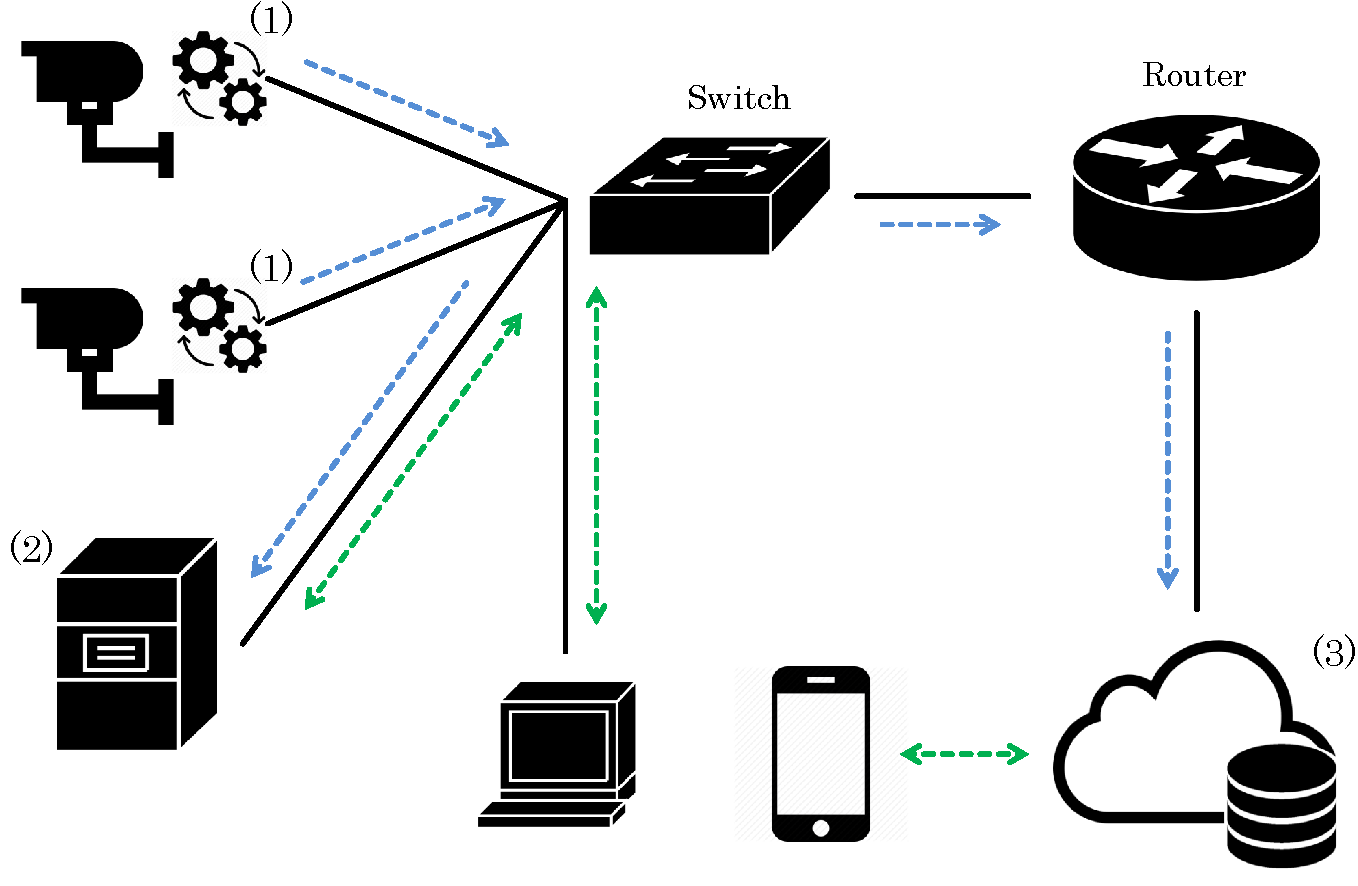
\includegraphics[width=0.8\textwidth]{graphics/cctv/cctvSystem/cctvSystem.pdf}
  \caption[Exemplary structure of a CCTV system.]{Exemplary structure of a CCTV system with two IP cameras. These devices preprocess (1) their captured data before streaming it (blue) to either a local (2) or cloud-based storage (3). Access to the stored video data (green) either stays in the local network or is done through the internet.}
  \label{fig:cctv_system}
\end{figure}

However, while the technology of cameras and the systems surrounding them changed over the years, the challenges still persist: Even while the above mentioned providers provide event detection, these events are merely filtered based on motion detection, therefore many events are constantly being detected, most of them being normal and not of interest. Traditional ways of anomaly detection in video requires either requires human monitoring of the video feeds 24/7, which is inefficient, or going over the stored video data in intervals to look out for anomalies. The latter one is not desired due to the delay until an event of interest is detected; this might even cost lives in some use case scenarios \cite{ferenbok2013hidden}. Also, because it is easier to setup cameras for CCTV systems, the number of video feeds that need to be analyzed in even small CCTV systems has also increased over the years \cite{vlahos2009surveillance}.  This increasing demand for automatic methods for analyzing the increasing quantities of video data that is continuously being generated, warrants the application of various machine learning techniques to detect anomalies. In the following section, we explain and discuss the types of anomalies and how they appear in video streams and how different anomaly detection techniques would work for the given problem and how they differ from each other.



% Anomaly Detection
\section{Anomaly Detection} \label{sec:anomaly_detection}

Anomaly or outlier detection, describes the recognition of patterns that do not comply with the general expected behavior, as illustrated in Figure \ref{fig:anomalies}. The research areas of thereof include machine learning, statistics, information theory, among many others and the application domains are also wide ranging and it is often non-trivial \cite{chandola2009anomaly}: Detected anomalies are not necessarily malicious activities in the context of a security application for example, but it could be the case, that these anomalous observations are merely an unknown and new, but a to be considered normal kind of pattern within the data. In addition, true anomalies might be detected as normal observations, if they are similar to past normal ones. This challenge increases, when normal and anomalous behavior evolves over time and the detection technique has to evolve with it. Although the application domains differ from each other, the challenges remain the same and this includes video anomaly detection (VAD) \cite{shin20203d}.

\begin{figure}
	\centering
	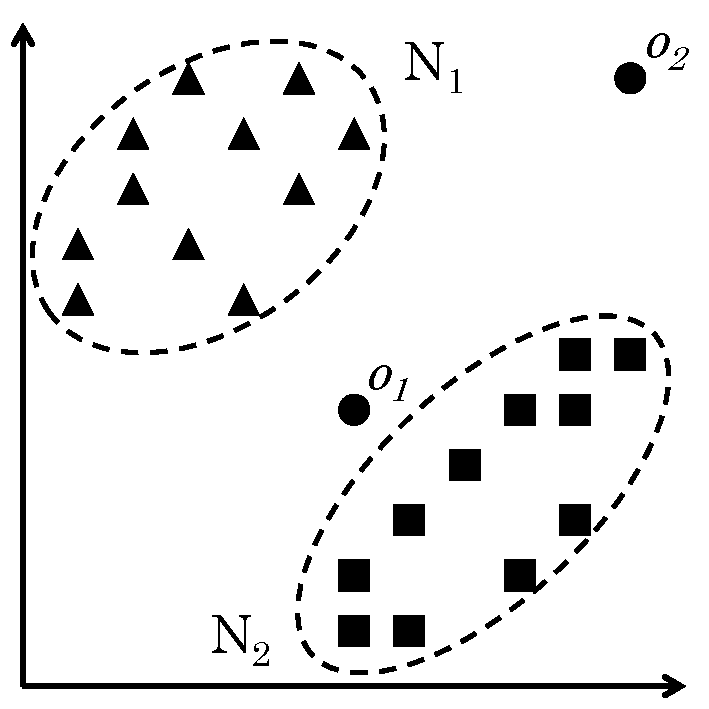
\includegraphics[width=0.39\textwidth]{graphics/anomalyDetection/anomalies/pointAnomaly/pointAnomaly.pdf}
  \caption[Example of outliers in a 2-dimensional data set.]{Example of outliers ($o_1$, $o_2$) in a 2-dimensional data set. \cite{chandola2009anomaly}}
  \label{fig:anomalies}
\end{figure}

In this section, we provide the categorization for the types of anomalies and how they relate to anomalies found in video streams. Due to their nature, a different definition of the types of anomalies based on object patterns is also added to that. For the detection of anomalies within video streams, different detection techniques could be used, determined by the existence and the properties of training data and how the video streams have to be analyzed. Therefore, a taxonomy of the different types of anomaly detection techniques is given, and the challenges that come with them for VAD are highlighted.


% Types of Anomalies
\subsection{Types of Anomalies} \label{subsec:anomaly_types}

An important aspect of anomaly detection is the nature of the (to be) detected anomalies. These can be divided into the following three categories \cite{chandola2009anomaly}:

\paragraph{Point Anomalies} \label{par:point_ano}
The simplest type of anomaly and often the main focus of many research on anomaly detection \cite{malik2014comparative}: These anomalies are considered anomalous on its own with respect to the rest of the data. See Figure \ref{fig:anomalies} for exemplary anomalies $o_1$ and $o_2$. In an example from an application domain, a point anomaly could be a credit card transaction, in which the amount spent is much higher compared to normal transactions. Point anomalies are often not of interest in VAD \cite{shin20203d}. This is because videos are considered spatio-temporal in nature, i.e. they do have a temporal component and the observations --- video frames, are heavily dependent on past and future frames, which results in many anomalies being either contextual or collective. However, they do exist and they can be artificially injected; for our evaluation data set that is presented in detail in Chapter \ref{chap:contribution}, we created a few of these anomalies, by adding flashing of lights during the recording.

\begin{figure}
	\centering
	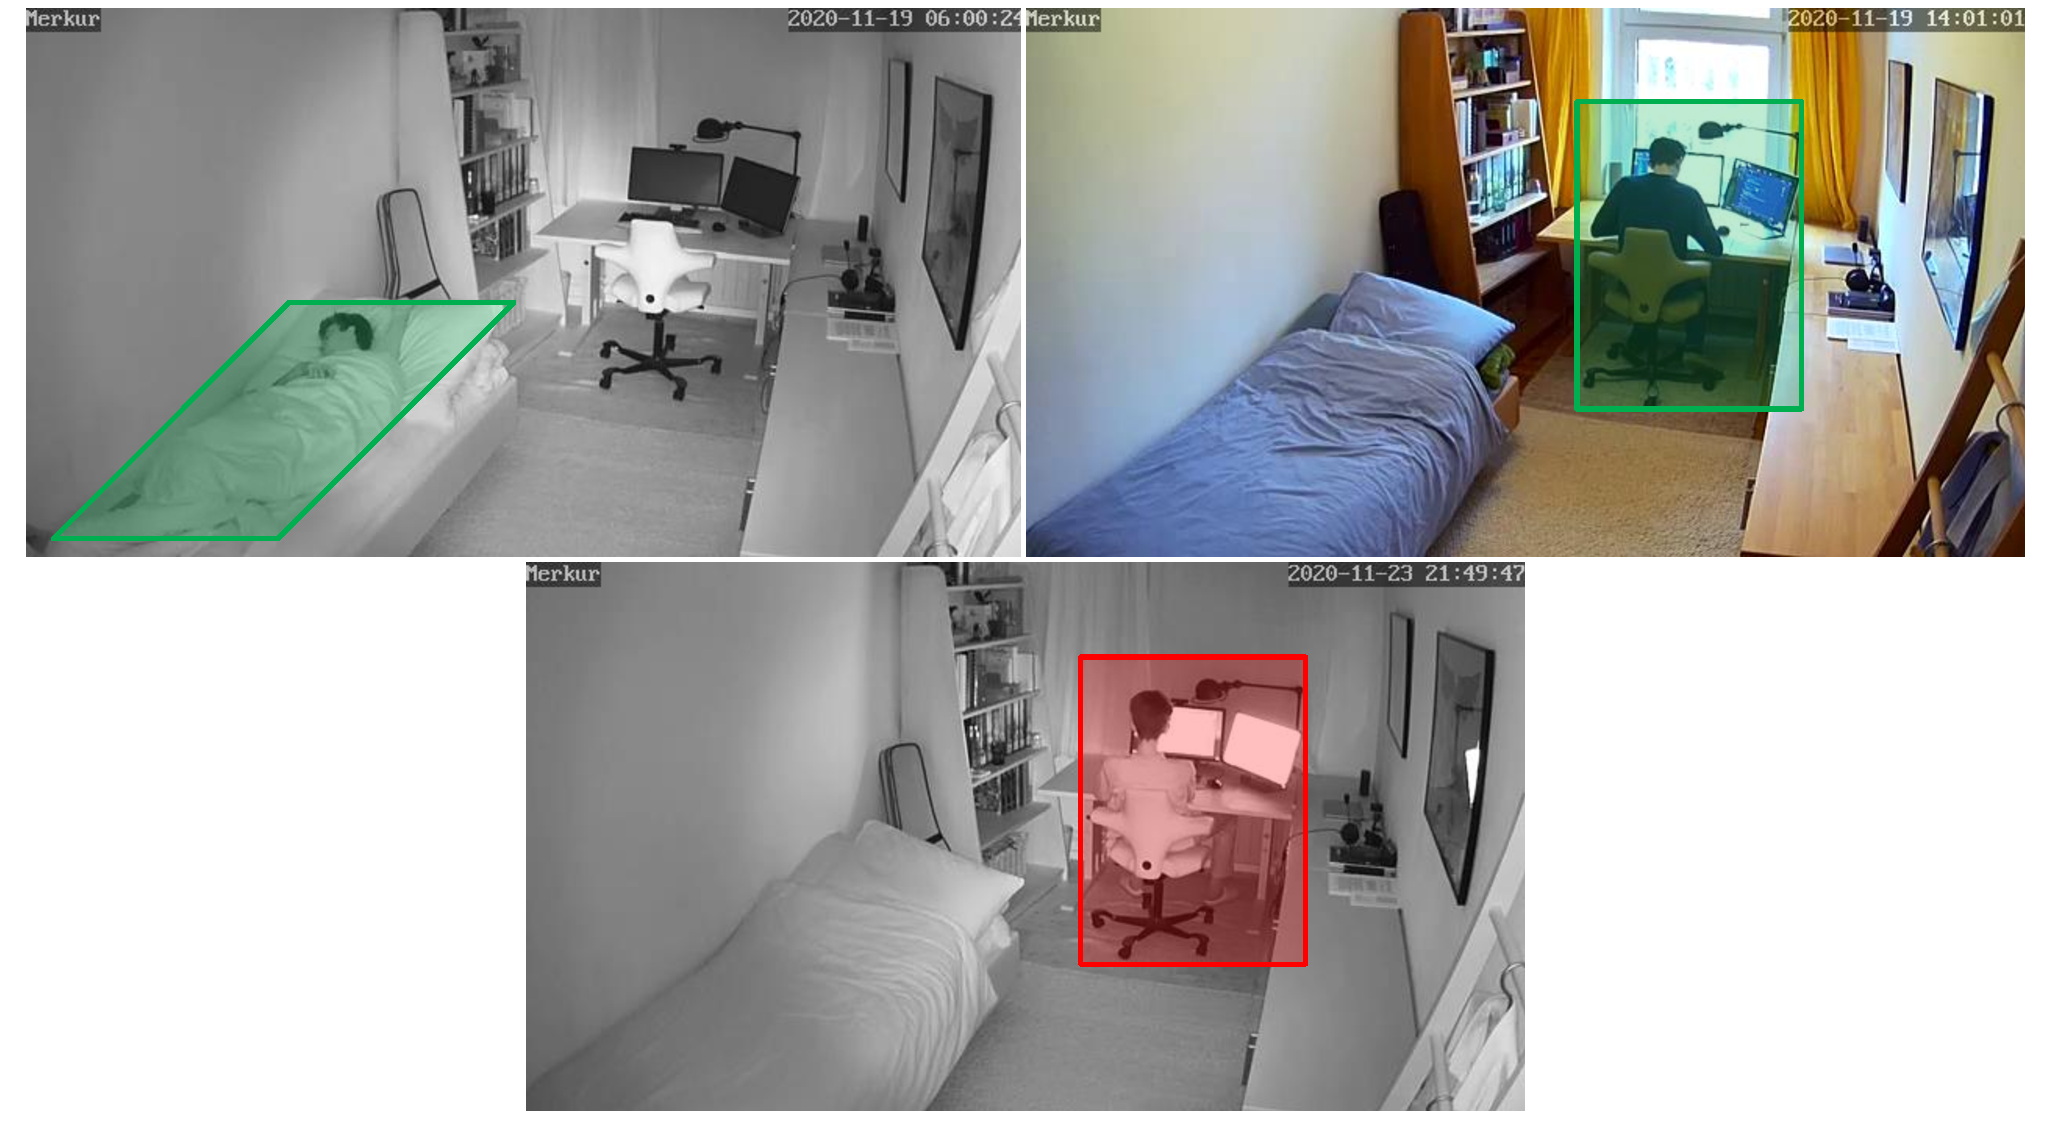
\includegraphics[width=0.68\textwidth]{graphics/anomalyDetection/anomalies/contextualAnomaly/contextualAnomaly.pdf}
  \caption[Contextual anomaly in video.]{A normal video frame during the night (upper left), the day (upper right), and a contextually anomalous one (lower middle). The object pattern marked in red is anomalous at night but normal under other circumstances.}
  \label{fig:contextual_vid_anomaly}
\end{figure}

\paragraph{Contextual Anomalies} \label{par:context_ano}
The notion of a context is usually induced by the data and the use case itself; they are most commonly found in time-series data which is spatio-temporal, same as video streams. These observations are considered normal during one context, while being anomalous in another. In case of a time series, the context can be directly encoded into the observation as a contextual attribute, which enables a detection system to detect these like point anomalies. In video however, defining a context is not always trivial, because there can be several different contextual attributes. First, patterns of objects in a video are often the case for contextual anomalies \cite{shin20203d}: A person walking on the cross-walk or sidewalk is considered normal, but when the same pedestrian is walking on the street it is an anomaly. Because both its appearance and motion pattern differ to the cars surrounding it. Second, as shown in Figure \ref{fig:contextual_vid_anomaly}, the behavior of the person can also depend on the light levels, or the time of day. In that case, when the curtains are closed and the room is not lit, a person sitting at the desk would be a contextual anomaly. Because the context is not explicitly given to the anomaly detection system, the model needs to learn to decode and identify the contexts of the video itself.

\begin{figure}
	\centering
	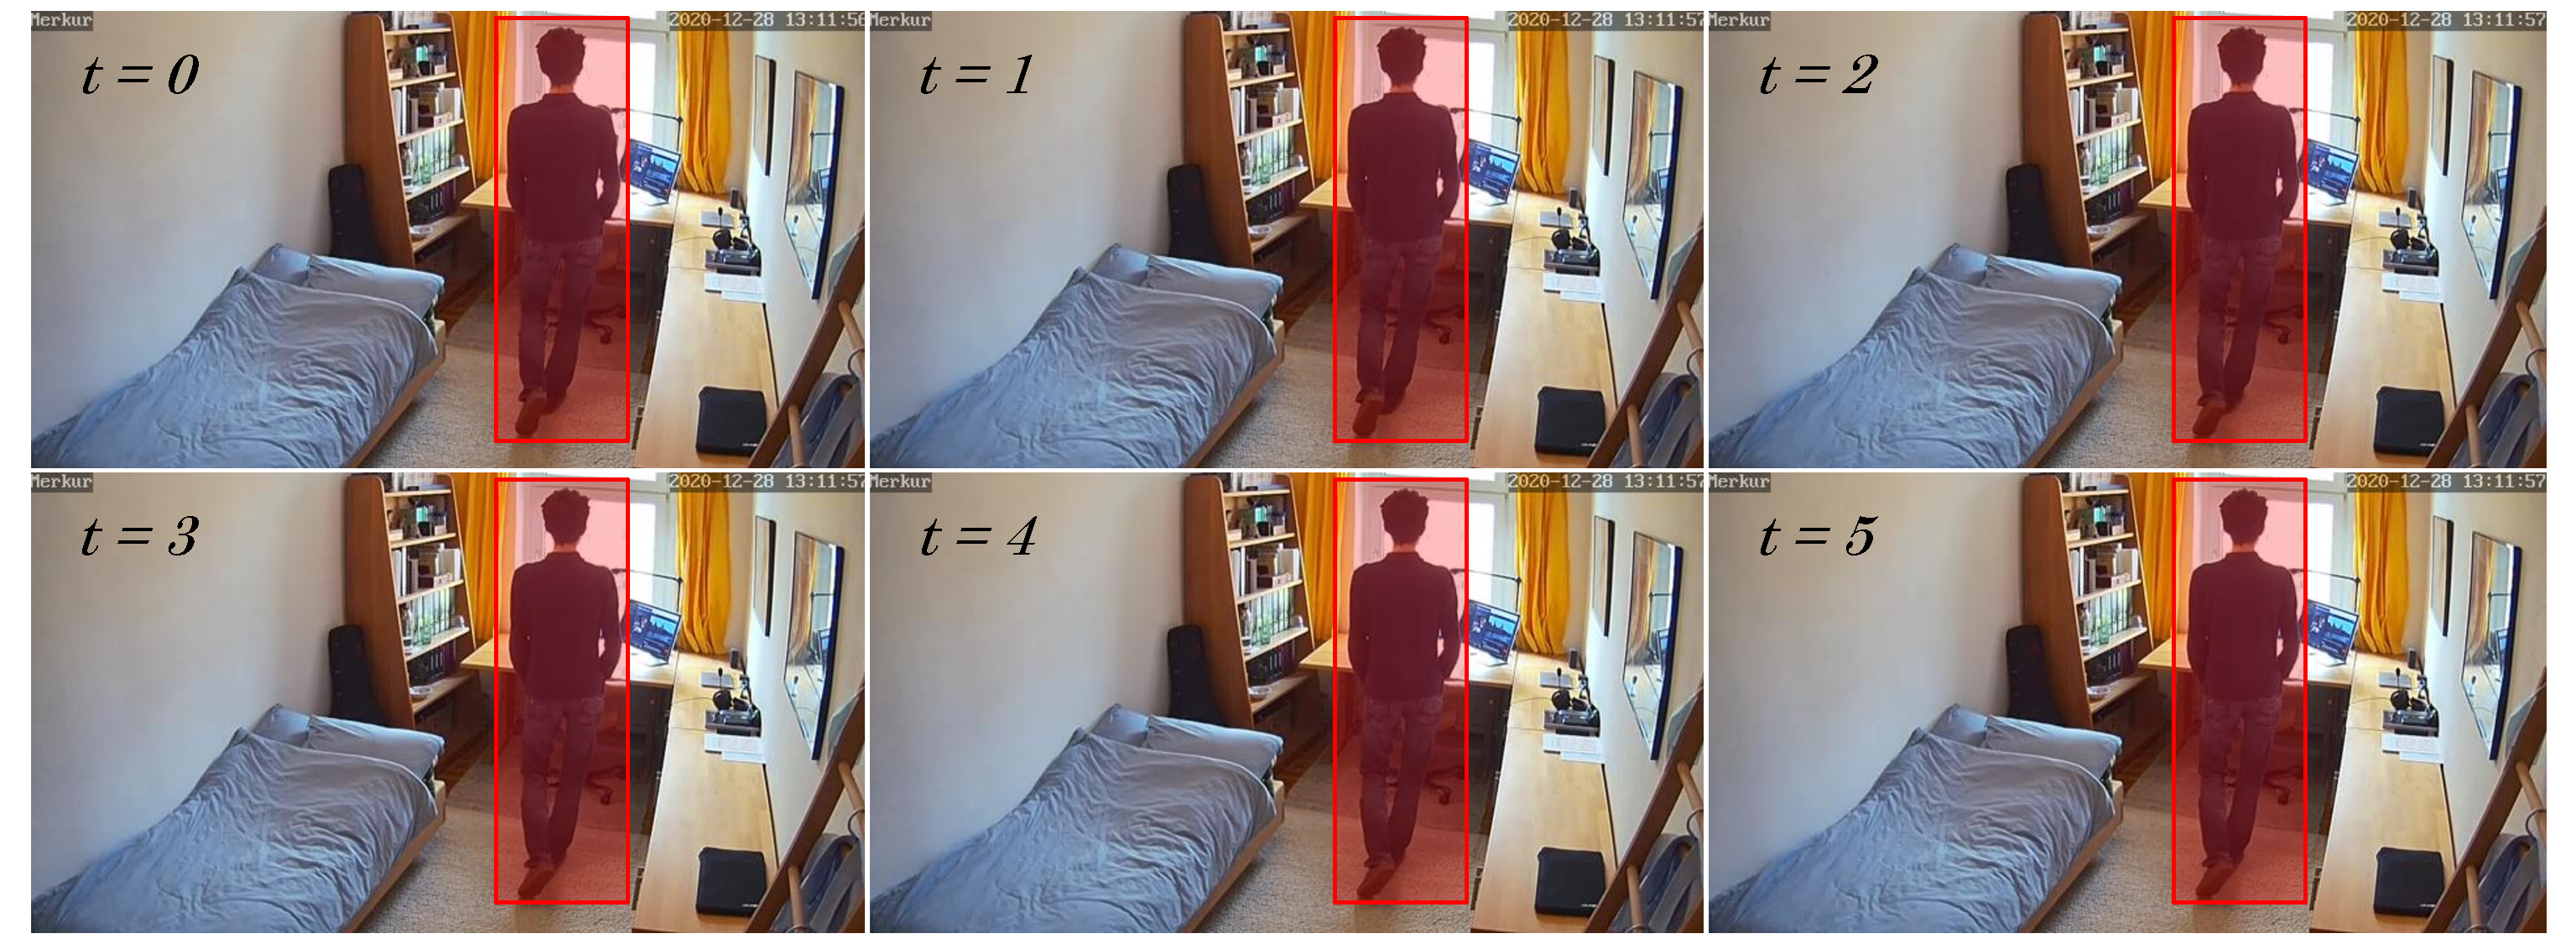
\includegraphics[width=1\textwidth]{graphics/anomalyDetection/anomalies/collectiveAnomaly/collectiveAnomaly.pdf}
  \caption[Collective anomaly in video.]{Individually these consecutive frames would be classified as normal, but together they are considered collectively anomalous. Although the person (red) seems to be walking, they are actually standing still.}
  \label{fig:collective_vid_anomaly}
\end{figure}

\paragraph{Collective Anomalies} \label{par:collect_ano}
Sequence data, such as video streams, sometimes has observations that look normal on their own, but with respective to observations that came before and will come after them, they are anomalous. An example from an intrusion detection system is the patterns of certain attacks, which consist of normal looking events \cite{chandola2009anomaly}. In video, collective anomalies can be detected by the motion patterns of the objects in a video: While the individual frames shown in Figure \ref{fig:collective_vid_anomaly} appear normal --- the person is walking from the camera away and towards the desk. Or so it seems. Because when one inspects the preceding and succeeding frames, one notices that the person is standing still. Vice versa, a very fast motion of an object that under normal circumstances moves more slowly could be considered a collective anomaly instead --- the collection of frames of that motion being part of that anomaly. Thus, a VAD system needs to learn to extract spatio-temporal features of objects within the video, i.e. it needs to learn how objects move under normal circumstances. Finally it is to note, that collective anomalies can also be contextual; a group of observations might be considered collectively anomalous in a specific context (e.g. a person running over the sidewalk), while in another context that motion pattern would be considered normal (e.g. the same person running over the sidewalk while it rains).


% Differentiating between Techniques
\subsection{Taxonomy of Anomaly Detection Techniques} \label{subsec:detection_techniques}

\paragraph{Detection Output} \label{par:detect_out}
The main requirement of an anomaly detection system is to report observations that appear anomalous. This either means that the system labels each observation in binary fashion, or that the underlying results are aggregated and smoothed over, to group the individual reports into events that are either normal or anomalous \cite{chandola2009anomaly, malik2014comparative}. Some detetion systems go further, and replace the binary output with a mapping to the specific kind of anomaly that was detected. Often however the results from the detection system is neither of the two but it is a score, ranging from $0$ and $1$, depending on the probability to which the model considers that instance an anomaly. In that case, the results are either mapped to a binary label by an expert, or a domain specific threshold function is defined by them. Our ADS for video presented in the next chapter does use a scoring technique internally, but due to the use of IFTM, a threshold is applied to the result which results in a binary label output \cite{schmidt2018iftm}.

\paragraph{Level of Supervision} \label{par:supervision}
Second, depending on the nature of training data and its labels --- in case of anomaly detection binary ones (normal or anomalous), it is decided which anomaly detection techniques can be used. This is because most outlier detection solutions need to be trained one some observations, before they can be used to detect outliers \cite{Bishop2006patttern, chandola2009anomaly}. And, depending on the detection approach, these have different requirements to the training data instances. The most transparent approaches to humans are policy-based, also called rule-based techniques \cite{huebscher2008survey}. By constantly checking if policies and rules, that were written by system administrators for example, are upheld, anomalies are detected if one or multiple of these rules are broken by the parameters of the system that is observed. Defining these rules can be simple for smaller systems and some application domains, but for others it becomes increasingly difficult if not impossible. But as already noted in the previous paragraph regarding the detection output, the output of a technique can be refined by the rules and policies of the human operator. For example in the case of the CCTV system by Netatmo that was presented in Section \ref{sec:cctv}, events are generated if successive frames differ from each other by a human set threshold $T$. Then, a facial recognition model is run on any detected humans and if these faces do not match with an internal database for that household that is monitored, the system interprets this behavior a breaking in policy and an alert is generated. However these underlying models are still trained in some fashion and therefore these techniques are not purely policy driven.

Then, there are supervised learning techniques; these require to be trained by labeled data of all existing normal and anomalous behavior. A prime example of this method is the nearest neighbor algorithm, that assigns every new incoming observation to the label of the nearest sample in the training data set \cite{cover1967nearest}. This techniques can provide the best results when there is a sufficient number of training data, but obtaining accurate and representative labels can be challenging, especially for surveillance data. For the rarest types of anomalies, this would imply some catastrophic events, that are very difficult to collect \cite{chandola2009anomaly}. In addition, labeling any kind of data is very expensive, due to the need of some human expert to label the observations by hand. For our use case as described in the following chapter, several days of unlabeled video data was available to us, but none of which was actually labeled.

This challenge of lacking labeled data transfers to the next kind of learning technique; semi supervised learning. In this case, models are either trained with a combination of labeled and unlabeled data, or only with the observations that show one type of class. In the latter case, a model based on the normal behavior of a system can be built \cite{malik2014comparative}. On the other hand, some models use forms of transfer learning to infer the labels of the remaining (unlabeled) training data, to refine the model further, after which it has been trained by the labeled observations \cite{shin2018cctv, shin20203d}. In Chapter \ref{chap:state_of_the_art}, we will discuss some research regarding these approaches and discuss how they differ from our own solution.

For unsupervised anomaly detection, no labels at all are available during training. These makes them widely applicable, because for training, raw data can be fed to them. However this does come with a price, because they often run under the implicit assumption, that anomalies are rare and thus are ``drowned out`` during training, because the normal data dominates the set. If this assumption is done falsely, the detection rate of these techniques will suffer \cite{chandola2009anomaly}. For VAD systems, this assumption is often made \cite{schlegl2017unsupervised, jamadandi2018predgan, akcay2018ganomaly, liu2018future} due to the high availability of raw data. Our proposed video generation model is trained in unsupervised fashion, as is IFTM in which the model is incorporated after training \cite{schmidt2018iftm}. 


\paragraph{Online or Offline} \label{par:online_offline}
Finally, anomaly detection algorithms can be divided into two groups, into which all algorithms that require input fall \cite{karp1992line}: Pure offline detection techniques require the entire batch --- data, that has to be analyzed beforehand. This can yield better results due to their encompassing view of all observations, but at a cost of being no longer able to detect anomalies in real-time, but only after these have occurred. Others group incoming observations into smaller sets called mini-batches and process these indivudally in a batch wise manner to solve this problem, but in return they lose some detection quality. The most responsive systems are online algorithms. These are especially useful for continuous streams of observations that have to be analyzed one step at a time. Video feeds generated by a camera are one of these use cases, because the size of the potential data set is technically infinite. Though, online techniques are more responsive compared to offline methods, they struggle especially at the start --- this is called the cold start problem, when their models are not that good due to the lack of sufficient training initially. Furthermore, context shifts within the data stream can occur, forcing the model that no longer represents the incoming data, to adapt to the new context. This requires the model to recognize the shift and then to either use a new model, or to forget older observations that are no longer relevant to the current state. These two groups should not be seen as binary --- training could be realized as a batch process over a set of observations that is known in advance, before the incoming stream of observations is classified in real-time. In some cases, the underlying model is also trained on a batch of data in advance, before it is further refined in stream-wise fashion, while also already classifying the new incoming observations. This kind of pre-training counteracts the cold start problem \cite{erhan2010does}.

The anomaly detection framework that is used in our approach --- IFTM, is flexible \cite{schmidt2018iftm}: Its threshold model can either be trained offline and is then fixed for the detection phase, or it can be continuously updated online-wise. But, because our model that represents the normal state of the video stream is trained in adversarial fashion until convergence \cite{goodfellow2014generative}, as explained in the following section, training of the entire system has to be done offline. Therefore the entire video ADS is doing training offline and detection will be done in an online manner.



% GANs
\section{Generative Adversarial Networks} \label{sec:gans}

Over the last years, research moved away from typical neural networks \cite{haykin1994neural} to more refined deep neural networks that are able to recognize high level concepts, such as objects in images or videos, audio waveforms containing speech, or the processing and understanding of written text \cite{bengio2009learning}. This change was also made possible due to the increasing power of modern hardware and distributed computing, which allowed an increase in complexity of the networks. The abstract underlying concepts remain the same however; the variables within a network are optimized following certain criteria that rate the quality of the outputs that the model produces. Backpropagation is then used to calculate the gradients, and these are then passed to an optimization algorithm to adjust the trainable parameters within the network.

With the increasing complexity and thus the increase in trainable parameters, there is the increasing risk that components of the inputs during training are directly copied into the network's parameters. Goodfellow et al. claim generative adversarial networks (GANs) overcome some of these challenges \cite{goodfellow2014generative}. GAN --- as the name suggests, consists of atleast two neural networks, that are adversaries in nature. As one can see in Figure \ref{fig:gan}, the generative model (the generator) is pitted against a counterpart (the discriminator). The latter one has to learn the properties of the training data and to distinguish real inputs that have these properties from synthetic ones. The generator on the other hand has to learn to trick its opponent into believing that its synthetic outputs are real enough to be labeled as not fake. 

\begin{figure}
	\centering
	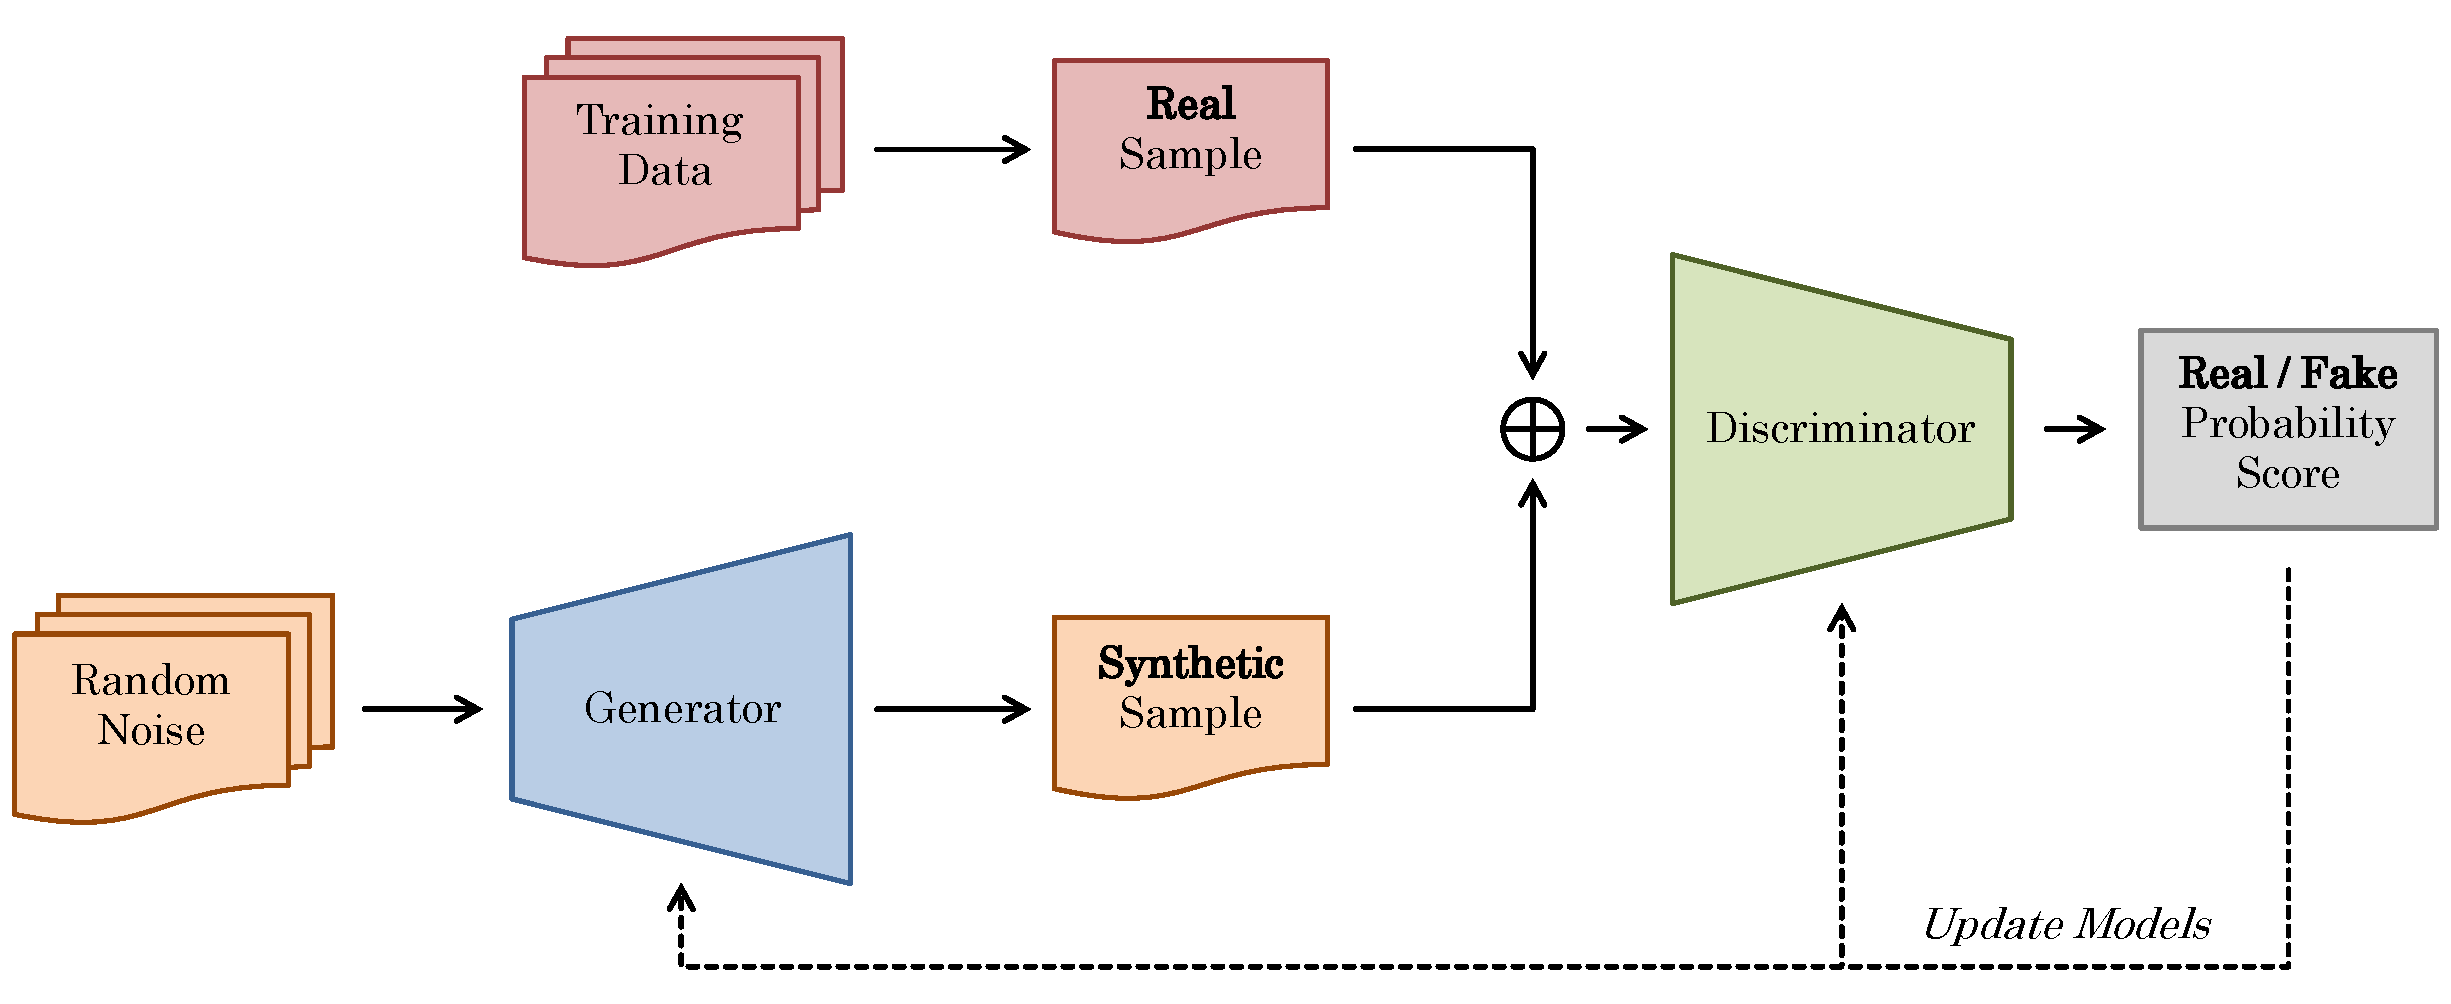
\includegraphics[width=1\textwidth]{graphics/gan/gan/gan.pdf}
  \caption[Structure of a GAN.]{Exemplary structure of a GAN. Synthetic samples are generated based on inputs sampled from random noise. Classification results for synthetic and training samples by the discriminator are used to tune the two models.}
  \label{fig:gan}
\end{figure}

This approach during training can be formalized into Equation \ref{eq:gan}, with the generator network being $G$ and $D$ being the discriminator: The first term describes the error of $D$ to recognize inputs $x$ sampled from the training distribution $p_x$, and labeling these as real ($D(x)=1$). Therefore the discriminator gains direct insight into the training data set. This is usually done in an unsupervised manner; the learning of any features and properties that make these observations real is the overarching goal during training. There are also variations of GAN in which the discriminator learns to not label inputs as either real or fakes ones, but to provide non-binary classification \cite{simonyan2014two, isola2016image}. The second term in the Equation refers to the sampling of $z$ from a normal distribution, that is passed to the generator to generate a synthetic output. This output is then classified by the discriminator. The goal of the generator is to minimize this term, i.e. $D$ must no longer be able to discriminate between real and synthetic data points. Meanwhile $D$ seeks to maximize it, labeling synthetic examples as fake ($D(G(z))=0$). Training of GANs is done iteratively; every step, a mini-batch is sampled from both the random distribution ($p_z$) and the training data ($p_x$) and both models are updated separately to optimize Equation \ref{eq:gan}.

\begin{equation} \label{eq:gan}
\min_G \max_D V(D,G) = \mathbb{E}_{x \sim p_x(x)}[\log D(x)] + \mathbb{E}_{z \sim p_z(z)}[\log(1 - D(G(z)))]
\end{equation}

Thus training GANs is a zero-sum game, in which both models have to improve in parallel. As $D$ becomes better in distinguishing real from fake examples, $G$ also improves in fooling its adversary, making the generated outputs more and more real. This way, the generator, without having direct access to the training data, learns general feature representations that mirrors the statistics of the training set. For example, if one trains a GAN with a database of human faces, the training examples are passed to the discriminator, and the generator will learn to generate real looking human faces from random input $z$. 

\paragraph{Common Failure Modes in GAN Training} \label{par:failure_modes}
Note that the convergence of Equation \ref{eq:gan} should not be one-sided \cite{zhang2018convergence}: If the two sides do not reach a balance during training, one of the two models will slowly minimize their error until the error of that model reaches zero, while the other reaches the error function's maximum. This not only stops improvement in training, but actively degrades the output: In case $D$ dominates during training, $G$ no longer is able to generate any outputs that might fool its counterpart and thus gets no hints on how to continue learning. Vice versa, if $G$ overpowers $D$, the generator usually learns some simple feature representation that the discriminator can not identify as fake. This can also result in generated outputs, that have a low error from the discriminator's point of view, but are very low in quality. Lastly, there is also the ``mode collapse``, in which $G$ no longer generates a large variety of different outputs, but ``collapses`` different input ($z$) to the same synthetic output. This happens if the generator is unable to learn a rich feature representation from the given inputs.

There are different approaches to solve the different failure modes \cite{roth2017stabilizing, zhang2018convergence}. They include the impairment of one model and the improvement of the other. This can be done by simply increasing or decreasing the number of trainable parameters of a model, i.e. adding and removing layers, lowering the dimensions of certain layers, etc.. But an impairment can also be realized by adding regularization layers, such as dropout layers \cite{hinton2012improving}: A dropout layer randomly sets a percentage of the input units of the next layer to 0, which forces the model to add redundancies in its parameters, thereby lowering its expressiveness. When weakening the discriminator, one can also randomly flip the labels of the data from which the discriminator trains from. This can either be done in one-sided manner, labeling real data points as synthetic, or for both classes equally. For solving the mode collapse problem, one can also increase the size of the latent input space. Finally, one can also tune the number of training steps, that each model does per training iteration. So for example, in case $D$ overpowers the training, $G$ is trained two mini-batches during each step, while $D$ is merely trained once.

Although Goodfellow et al. have formally proven \cite{goodfellow2014generative}, that training will always converge, if both models have enough capacity and they are both trained each step until having reached an optimum, this is not necessarily an equilibrium in which both discriminator and generator continuously improve. If the generator succeeds perfectly, while also generating perfect synthetic data points, the discriminator has a 50\% accuracy; the prediction is essentially a coin toss. This feedback however can create an oscillating error, that may start the generator to train on false feedback, thus worsening the generator once more and risking a collapse in training. This can be solved by early stopping, i.e. stopping training once a stable equilibrium was achieved \cite{yao2007early}, but there are also other variants that change the way training is done in dynamic fashion to adapt to the changes in objectives \cite{zhang2018convergence, thanh2020catastrophic}.\\

Our proposed ADS system uses a GAN, namely the generator after training is completed, to model the properties that normal video observations have. Therefore, we design $G$ and $D$ to generate and discriminate videos, respectively. The challenges in training GAN were in some part also encountered during the evaluation of our approach; these challenges are discussed in Chapter \ref{chap:contribution} and \ref{chap:results}. Note that the idea to use GANs for video generation, forecasting, and VAD are not novel; in Chapter \ref{chap:state_of_the_art} we provide an overview over similar approaches to ours. 

The rest of this section provides a short introduction into a constrained architectural variant of GAN, that is more stable for some application domains --- especially image and video generation. Lastly, we provide an overview over a subtype of GANs that accept additional inputs, which is necessary for video generation forecasting.


\subsection{Deep Convolutional Generative Adversarial Networks} \label{subsec:dcgan}

There are different challenges when designing GANs --- some of them are highlighted in Paragraph \ref{par:failure_modes}, which makes the designing of these adversarial models particularly challenging. Due to that, new models are usually based on already existing constrained architectures, that were proven and evaluated to work on different application domains. Deep convolutional generative adversarial networks (DCGANs)\nomenclature{DCGAN}{Deep convolutional generative adversarial network} \cite{radford2015unsupervised} build on the success of regular convolutional neural networks (CNNs)\nomenclature{CNN}{Convolutional neural network}. CNNs have a wide array of applications when processing some form of spatial data \cite{ciregan2012multi}. For example when processing images, pixels that are neighbors are relevant to each other when extracting features out of that image. By sliding kernel filters over an image and aggregating the neighboring pixels values, one can create a number of feature maps from a single input. These feature maps can be aggegrated or further processed by additional convolutional layers to extract lower level features, to be used for image classification or object recognition \cite{krizhevsky2017imagenet}. One can also replace these 2-dimensional convolutions with 3-dimensional ones \cite{tran2015learning, ji20123d}, which allow a model to understand spatio-temporal features. One of the application domains for these is video processing \cite{simonyan2014two}.

\begin{figure}
	\centering	
	\begin{subfigure}{\textwidth}
    \centering
    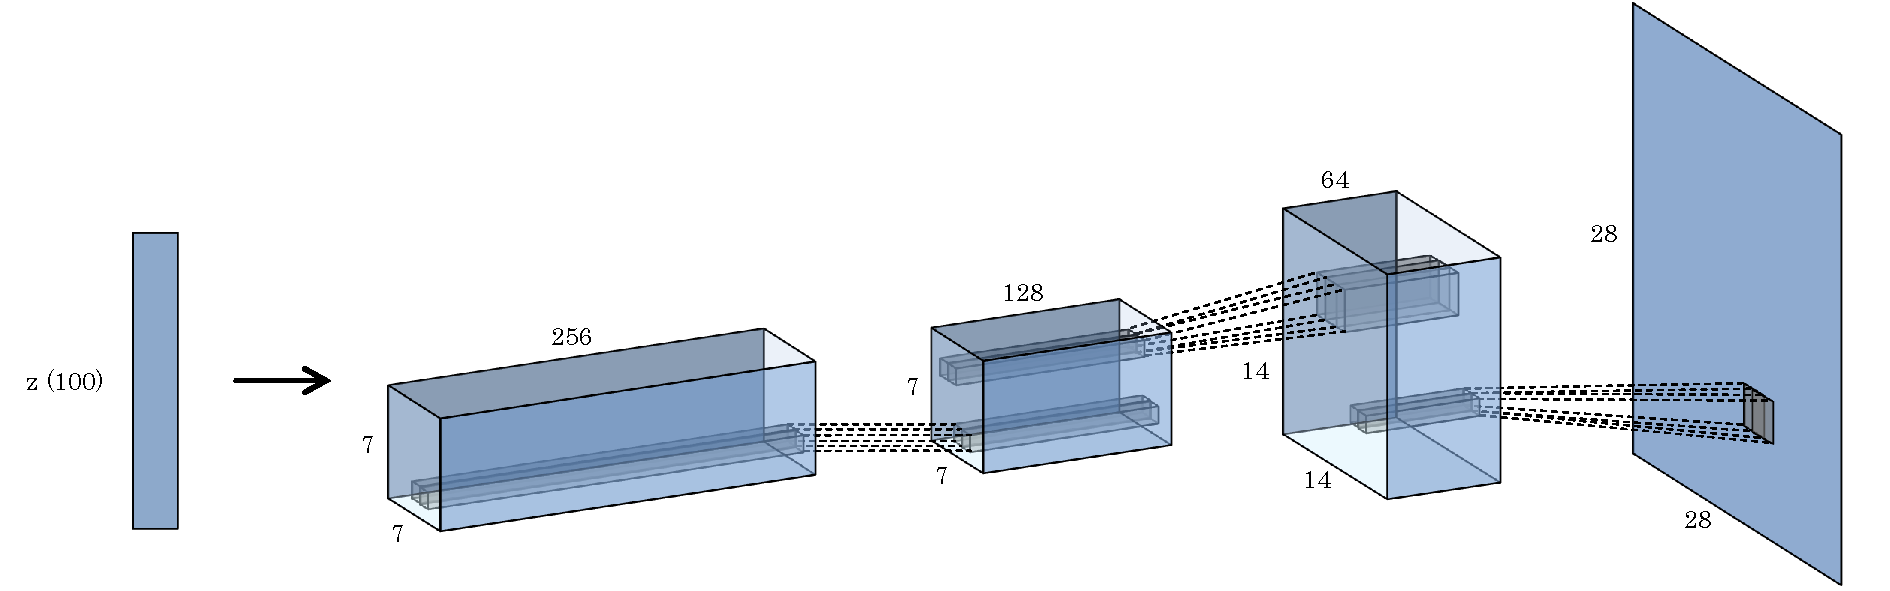
\includegraphics[width=1\textwidth]{graphics/gan/dcgan/dcgan_g.pdf}
    \caption{DCGAN generator.}
    \label{subfig:dcgan_g}
  \end{subfigure}
 
	\begin{subfigure}{\textwidth}
    \centering
    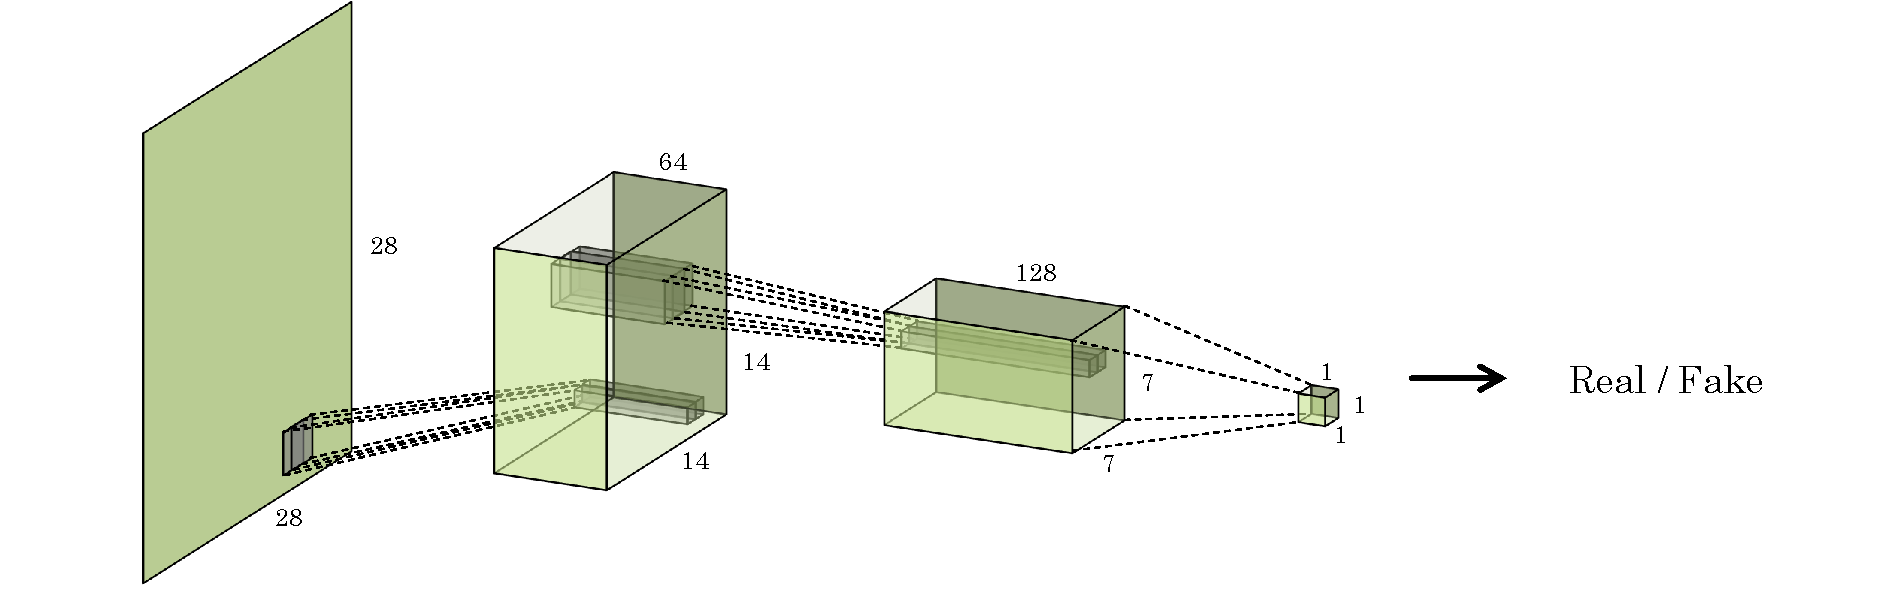
\includegraphics[width=1\textwidth]{graphics/gan/dcgan/dcgan_d.pdf}
    \caption{DCGAN discriminator.}
    \label{subfig:dcgan_d}
  \end{subfigure}
  
  \caption[Constrained DCGAN architecture.]{Exemplary DCGAN for image generation and discrimination. A 100-dimensional random latent vector is projected and reshaped to a small convolutional representation but with many feature maps (pictured by the depth of each cuboid). Three fractionally-strided spatial convolutions then upsample the encoded representation into a $28 \times 28$ grayscale image. The discriminator reverses this process, downsampling the image to a 1-dimensional output.}
  \label{fig:dcgan}
\end{figure}

Radford et al. combine CNNs with their counterpart --- de-convolutions often called, that instead of increasing the number of filters while usually decreasing the size of the dimensions, do the opposite. This technique can be used for upscaling \cite{zeiler2010deconvolutional}. The discriminator ($D$) in this architecture is therefore a CNN-based classifier, and the generator ($G$) creates synthetic output by upsampling the latent input to the output size. This results in two symmetric models as illustrated in Figure \ref{fig:dcgan}\footnote{The DCGAN in the figure is modeled after the one used in the DCGAN TensorFlow tutorial (\url{www.tensorflow.org/tutorials/generative/dcgan}), which generates ``hand-drawn`` MNIST digits \cite{lecun2010mnist}.}. DCGAN however has more constraints for its architecture: First, pooling layers, that are usually applied after a convolutional layer to aggregate the outputs, are replaced by strided (for $D$) and fractionally-strided (for $G$) convolutions. Changing these deterministic layers to something that can be trained, allows the models to learn their own downsampling and upsampling, respectively \cite{springenberg2014striving}. Any fully connected hidden layers are also removed, except for the input of the generator and the output of the discriminator. Batch normalization layers \cite{ioffe2015batch} are used after every layer in both $D$ and $G$ except for the input and the output, respectively. According to Radford et al., this prevents early mode collapse \cite{radford2015unsupervised}. Using only bounded activation functions, such as ReLU \cite{nair2010rectified} for the generator and Leaky ReLU \cite{maas2013rectifier} for the discriminator instead of maxout activation like in original GAN, except for the generator output layer that uses the hyperbolic tangent activation, also creates better results when using GANs for spatial data \cite{radford2015unsupervised}. Finally during training, no pre-processing steps for the input data was taken, besides scaling it to a range of $[-1,1]$. For the optimization of the trainable parameters the Adam optimizer \cite{kingma2014adam} with tuned hyperparameters was chosen.

Although the reference architecture on which our approach built is based on DCGAN, we evaluate different hyperparameter combinations for the batch size and the optimizer's learning rate for the adversarial training of our model. Both our model, use case, and data differ, while the parameters for DCGAN in the original paper were chosen for specific data sets, mainly image and face generation. The underlying idea of the DCGAN architecture is preserved though. The differences of the chosen parameters to those described here are further expanded on in the next chapter.


\subsection{Conditional Generative Adversarial Networks} \label{subsec:cgan}

Lastly it is to note, GANs are not only useful for generating real looking synthetic images and other outputs, but by tuning the function which has to be optimized, one can set different goals for the models that are trained. Mirza and Osindero adapt Equation \ref{eq:gan} to condition both models on predetermined, non-random input, resulting in Equation \ref{eq:cgan} \cite{mirza2014conditional}. $y$ in that case can be seen as additional information which $G$ and $D$ use to generate or discriminate data. In case of the generator this means, that the sampled noise $z$ is combined with $y$. Because the discriminator gets $y$ as an input as well, $G$ will implicitly learn to generate outputs, that somehow relate to $y$. In case of MNIST digits \cite{lecun2010mnist}, this could mean telling the generator to generate a specific type of digit ($y$). But this can also be extended by giving the conditional generative adversarial network (C-GAN)\nomenclature{C-GAN}{Conditional generative adversarial network} a list of tags that should be used as a baseline to generate an image from.

\begin{equation} \label{eq:cgan}
\min_G \max_D V(D,G) = \mathbb{E}_{x \sim p_x(x)}[\log D(x|y)] + \mathbb{E}_{z \sim p_z(z)}[\log(1 - D(G(z|y)))]
\end{equation}

For out approach, we use a variant of this method to give the generator conditional input in the form of spatio-temporal data (video frames), and it will learn to generate future frames from it. This is explained in detail in the following chapter, Section \ref{sec:cvgan}. % 10

\chapter{Contribution} \label{chap:contribution} % 30-40 pages

In this chapter, the use case and its challenges are presented, before we go into detail of how the GAN has to be adapted to allow forecasting of future frames in video. We also provide a step by step analysis of our modifications to the GAN that we used as the baseline architecture for our final model. Afterwards, we present our modifications to IFTM and how our GAN model is integrated into the framework. Then, our large-scale evaluation data set is presented and formally analyzed for some of its properties. The chapter closes with a summary of how all of this is combined into our anomaly detection system. An implementation of the different GANs, IFTM, and the rest of our analysis framework is available online\footnote{\url{https://github.com/fshofmann/video-anomaly-detection}}.



% Use Case CCTV Anomaly Detection
\section{CCTV Use Case} \label{sec:use_case}

As we described the challenges of video anomaly detection (VAD) in CCTV systems in Section \ref{sec:cctv} and explained why this kind of analysis requires the automated processing of a high amount of video data that is produced continuously, we decided to evaluate our VAD approach for the following CCTV related use case: A CCTV IP camera\footnote{\href{https://www.upcam.de/en/ip-cameras/upcam-cyclone-indoor/upcam-cyclone-hd-eco/176/upcam-cyclone-hd-eco-black-all-in-one-surveillance-camera}{upCam Cyclone HD eco}} for interior surveillance is stationed in a home office to monitor the behavior and changes of the person working there. This location was chosen by us both due to the current ongoing pandemic  and any privacy concerns that may arise when recording third parties without their knowledge: According to the German Federal Data Protection Act the recording of such is only allowed in reason if only private property is monitored and the people recorded on video have explicitly given their consent \cite{brd2017fdpa}. Furthermore the proportionality has to be considered as well. To avoid any legal troubles, only the person working in the home office and the people living in the same household were captured by the camera.

The camera's position, viewing angle, direction, and field of view is overall static. This results in a more or less static scene as shown in Figure \ref{fig:room}: In the middle, one can see the desk and the office chair, surrounded by a shelf from the left side and a lowboard from the right. A bed is also present in the room. The person working there usually sits at the desk, moves in and out of the room and also sleeps in the mentioned bed during the night. Writing utensils and papers are sometimes stored on the lowboard and desk next to them. Occasionally other people enter the room, but mostly the working person is the only one present. Finally in the top right, a timestamp is attached to every video frame. 

\begin{figure}
	\centering
	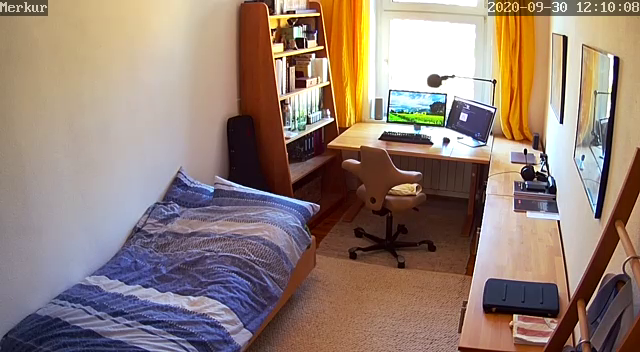
\includegraphics[width=0.9\textwidth]{graphics/cctv/room.png}
  \caption[View of the monitored room.]{Static view of the (empty) monitored room.}
  \label{fig:room}
\end{figure}

The IP camera's video feed is streamed via RTSP to a network attached storage and stored on a 30 day ring-buffer. The video stream is segmented  into one hour-long videos, with a resolution of $640 \times 352$ and a varying FPS of 2.5--5. The variance is explained by the (grayscale) night vision mode, that has fewer frames per second than the colored day vision. This results in the generation of around one gigabyte of unfiltered and unprocessed video data per day. We will expand on the properties and the preprocessing of the collected video data in Section \ref{sec:dataset}.\\

When using an anomaly detection system (ADS) to identify anomalous frames in that video stream, one has to learn and identify the different normal object patterns that people and objects in that video feed have. As explained in Section \ref{subsec:anomaly_types}, understanding the context in which an event is happening is often as equally important as the event itself. And to identify collective anomalies in the video, one has to analyze frames in context with their predecessors. But, due to the varying frame rate, it is difficult for a model to understand how much time truly has passed --- it could extract that information from the timestamp, but this would be costly. Instead, the video frame rate has to be stabilized. In addition, the resolution is impractical for some kind of models, which requires a specific constrained input format. Since there are no labels attached to any frames of the video data available, training of the ADS must be done in an unsupervised mode. This means one has to assume that the raw video data is mostly considered normal and that the underlying model of the ADS will not be corrupted by any potential anomalies found during training. Ideally, these anomalous properties and features are forgotten and cast away by a model that should only represent normal features. 

Finally during the detection phase after the training of the model is completed, we only want to process frames of the (theoretically infinite) video stream once: The detection method is required to label each frame of the video, using only the preceding frames and its knowledge of the training data. This creates the need of several modifications to the underlying model which IFTM uses to represent the normal state and how the data has to be processed --- this will be described in the following section.



% C-GAN for Video Prediction
\section{C-GAN for Video Forecasting} \label{sec:cvgan}

In this section we describe and discuss our model for video generation forecasting. The model's characteristics are based on the generative adversarial network for video (VGAN) by Vondrick et al. \cite{vondrick2016generating}. During every modification step, we first present how the original architecture was designed, for what it was intended, and why and how we adapted it. First, the general VGAN architecture is modified, before we continue with its conditional version (C-VGAN)\nomenclature{C-VGAN}{Conditional generative adversarial network for video}. Finally we will present our proposed modification to C-VGAN to accept spatio-temporal data, i.e. multiple video frames. Each of the adapted models from the intermediate steps is fully functioning on its own, although not fully evaluated, because it is not of interest to the use case.


\subsection{VGAN} \label{subsec:vgan_mod}

Building on the successes of GANs and the constrained DCGAN architecture, that leverages large amounts of unlabeled images to generate realistic looking ones, Vondrick et al. propose a novel generative model for video \cite{vondrick2016generating}: Videos with scene dynamics can be dissected into a static background that determines the scene and a dynamic foreground, that is spatio-temporal in nature. Explicitly modeling this property in videos by using a two-stream architecture for the generator, allows the model to learn to untangle these components from each other. This is helpful for example, when the same object dynamics could occur in front of different static scenes. The model learns to generate these two pathways in an unsupervised manner, so when combined following Equation \ref{eq:vgan}, the resulting videos seem real.

\begin{equation} \label{eq:vgan}
G(z)=m(z) \odot f(z) + (1-m(z)) \odot b(z)
\end{equation}

The first of the two streams is spatio-temporal and its output consists of two parts: The actual moving foreground ($f$) and the spatio-temporal mask ($m$) of it. The latter selects or deselects pixels of foreground and background, so moving objects do not overlap parts of the back ground when foreground and background are merged together. To model the temporal information in video, fractionally-strided 3D convolutions are used instead of 2D ones. In addition, the kernel size of the convolutional filter is $4$ along all three dimensions instead of $5$ with a stride of $2$. An exception is the first de-convolutional layer, that instead uses a kernel size of $1$ but a higher stride to upscale the 100-dimensional Gaussian input ($z$) to the fitting size. Convolutional filters range from $512$ for the first layer, to $64$ and then $3$ (RGB color channels) for the last one, halving at every step of the stack. The same structure is used for the background stream ($b$), but because it only has to produce a static image, spatial convolutions without the temporal component are used. Everything besides that matches the foreground stream. As in the DCGAN architecture, the hyperbolic tangent activation function is used for the output layer, except for the mask that uses sigmoid activation. Note, that when aggregating the three tensors $f$, $m$, and $b$ into the final generated video, $b(z)$ has to be transformed into a 3D output to match the other tensors. This is achieved by replicating it across the time dimension, therefore being a static video of $n$ times the same frame. Something similar has to be done to $m(z)$; the mask does not have RGB channels but is only in a range of $[0,1]$ per pixel. So that singleton dimension has to be replicated across the three color channels to match background and foreground output.

For the discriminator, which also follows the DCGAN architecture, the foreground stream is reversed, downsampling a given video to a binary output (real/fake), by repeatedly applying strided spatio-temporal convolutions to the video. Their model produces and discriminates $64 \times 64$ videos that have 32 frames --- little over a second long, and it is used to generate real looking videos from random Gaussian input. As a second alternative application, the discriminator is extended to a K-way classifier to learn action recognition.\\

\begin{figure}
	\centering
	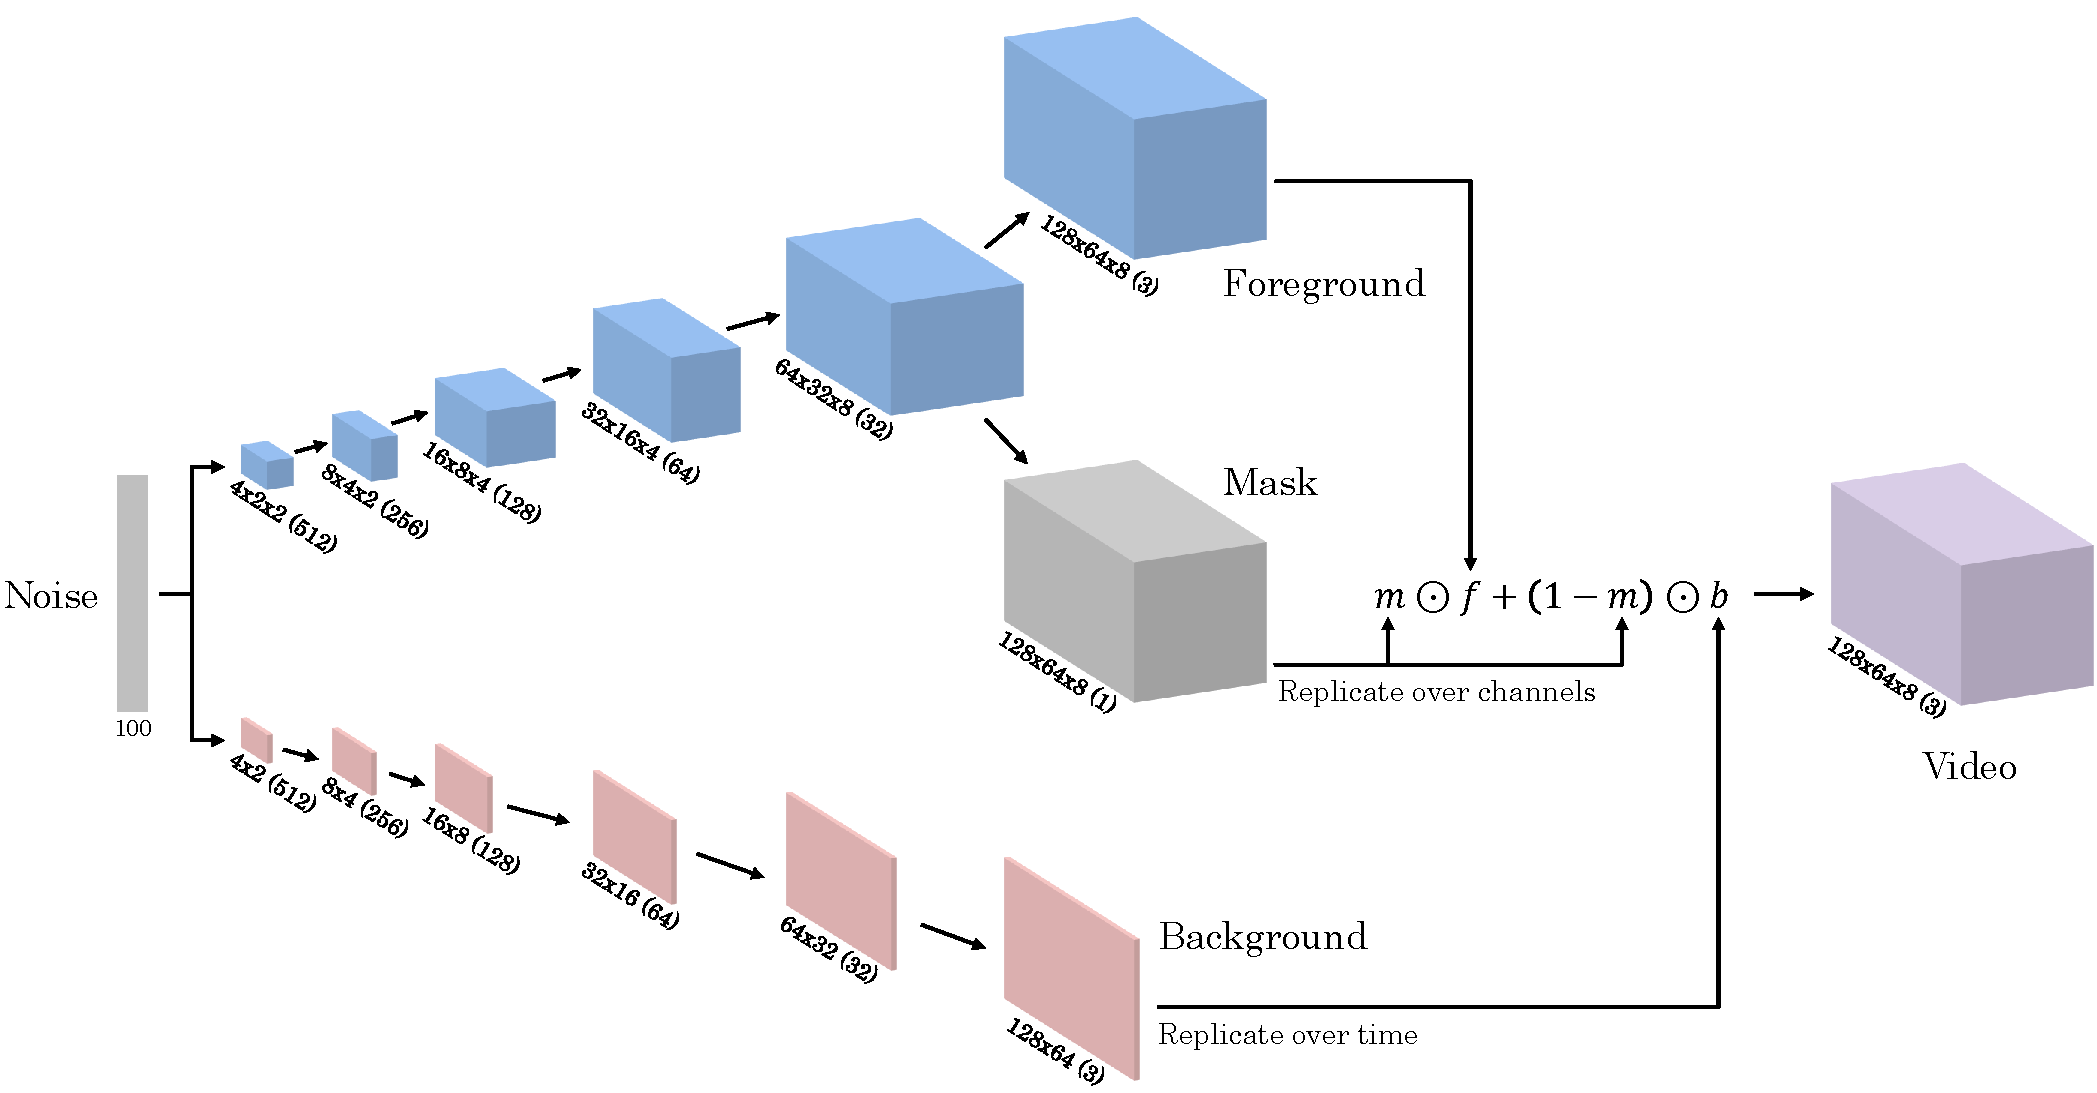
\includegraphics[width=1\textwidth]{graphics/gan/vgan/vgan/vgan_g.pdf}
  \caption[Adapted two-stream video generator network.]{Adapted VGAN generator \cite{vondrick2016generating}. A 100-dimensional random latent vector serves as input for two streams; a dynamic foreground using fractionally-strided spatio-temporal convolutions, and a static background of fractionally-strided spatial convolutions. The number in parentheses is the number of channels for each output, equal to the number of convolutional filters. As the generated video is in RGB, it does have three channels.}
  \label{fig:vgan_g}
\end{figure}

\paragraph{Modifications to VGAN}
For our modifications to VGAN shown in Figure \ref{fig:vgan_g}, the generator had to be adapted to our data first. During preprocessing of our data set as will be explained in Section \ref{subsec:dataset_preprocessing}, the video format was reduced to $128 \times 64$ and the frame rate was stabilized to 5 frames per second. Because this is one sixth the frame rate while the size of a frame has effectively doubled compared to the $64 \times 64$ that VGAN originally produced, it was decided that our generator shall generate videos with a length of $\sim 1.5$ seconds or 8 frames. This still results in less total pixels that need to be generated for a final space-time cuboid (video). On the other hand, the complexity of the background in fact increases, because it doubles in size. Therefore taking the loss and rise in complexity into account, one additional fractionally-strided convolutional layer is added to each stream, while the size of the first convolutional layer is slightly reduced. From $4 \times 4$ in the original VGAN to $4 \times 2$. Furthermore, because 8 frames instead of 32 have to be generated, the stride value along the time axis is only 2 every other convolutional layer. This gives the foreground stream enough space to upsample the frame information. In addition, because according to recent research even-sized convolutional kernels lead to distortions in the output \cite{wu2019convolution}, we change the convolutional layer's kernel size to $3$ across all relevant dimensions for both discriminator and generator. Instead of reshaping the input and feeding it directly into the first convolution, one dense layer for each stream upsamples the latent code to the input size of the first convolutional layer. Therefore, rather than having a kernel size of $1$ and being used as a matrix multiplication to reshape the input \cite{radford2015unsupervised}, the first convolutional layer is already being used for actual convolutional filters with a kernel size of $3$. Finally, weights in the generator network that precede ReLU activations, were not initialized with Gaussian noise ($\mu=0$, $\sigma=0.01$) like in the VGAN or DCGAN architecture. These weights are instead initialized with He normal, a truncated version of a normal distribution with an adaptive standard deviation. With the ReLU function being only positive, this helps with the quality and the convergence speed \cite{he2015delving}. The final convolutional layers' weights in the foreground with hyperbolic tangent and sigmoid activation are on the other hand initialized using the Glorot uniform initializer. The normal distribution used has an adaptive variance, balancing the variance of the input with the output's variance of the layer, which works especially well for these kinds of activations \cite{glorot2010understanding}.

\begin{figure}
	\centering
	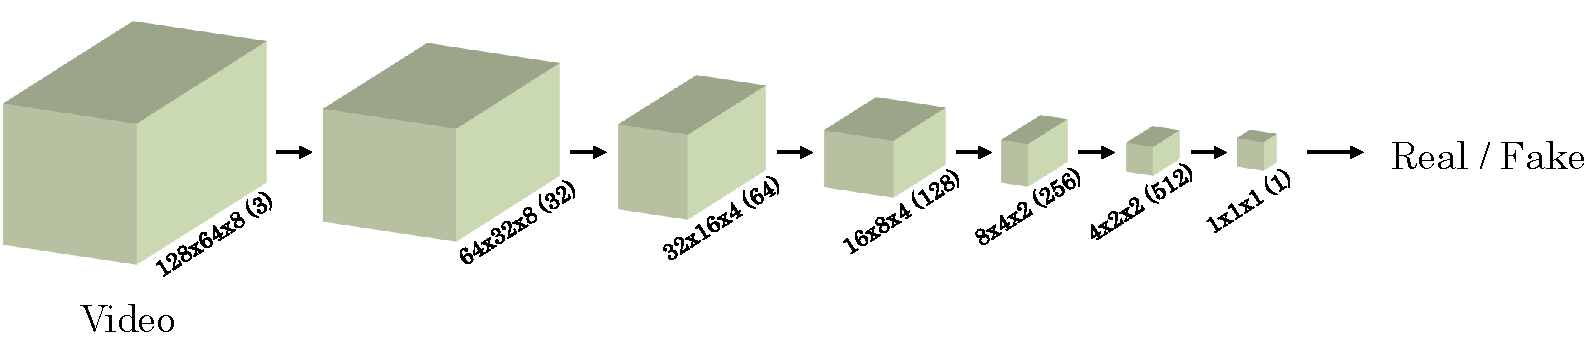
\includegraphics[width=1\textwidth]{graphics/gan/vgan/vgan/vgan_d.pdf}
  \caption[Adapted video discriminator network.]{Adapted VGAN discriminator \cite{vondrick2016generating}; a CNN-based classifier being the reverse of the generator foreground stream. The number in parentheses is the number of channels for each output, equal to the number of convolutional filters.}
  \label{fig:vgan_d}
\end{figure}

Our discriminator, as the original VGAN discriminator model, is the reverse of its counterpart's foreground stream: A spatio-temporal, CNN-based, video classifier with one fully connected neuron for the output. As seen in Figure \ref{fig:vgan_d}, videos are downsampled from $128 \times 64 \times 8$ to $4 \times 2 \times 2$, with the time dimension only halved at every second step in the convolutional stack, as it was done in the generator model.

This model, when trained using unlabeled video data, should only be able to generate (and discriminate) normal video clips of 8 seconds, if the training data is mostly normal. However, it is unfeasible to utilize the generator as a representation of normal behavior, because its outputs are impossible to be compared to the current state of the system: It simply generates random normal looking videos based on random input; this could be videos both during nighttime or daytime even. The discriminator may be of interest because of its ability to distinguish real videos from synthetic ones, but only if one can assume that anomalous observations in video seem ``fake`` to the discriminator. However, this assumption is risky --- the discriminator was trained to learn the properties of the generator network. Thus in the following section, we will look into a modification of VGAN for future frame prediction.


\subsection{C-VGAN} \label{subsec:cvgan_mod}

Vondrick et al. further refined their model to allow generation of a video based on an input frame \cite{vondrick2016generating}: In their published work, they achieved that by attaching a convolutional network as an encoder to the front of the generator network. The encoder mirrors the background stream but is reversed, encoding the $64 \times 64$ frame into latent code ($4 \times 4$, with $512$ channels), that both foreground and background stream then use to upsample from instead of the Gaussian noise. The first convolutional layer in the foreground pathway is this time used to upscale the latent spatial code into a spatio-temporal one (from $4 \times 4$ to $4 \times 4 \times 2$). This is accomplished by using a convolutional kernel of size $1$, but a stride of $2$ along the time axis. The function that has to be optimized during training is also extended with an additional loss term to force the generator to reconstruct the input:

\begin{equation} \label{eq:cvgan}
\begin{aligned}
\min_G \max_D V(D,G) = & \mathbb{E}_{x \sim p_x(x)}[\log D(x)] + \mathbb{E}_{x_0 \sim p_{x_0}(x_0)}[\log(1 - D(G(x_0)))] \\
+ & \mathbb{E}_{x_0 \sim p_{x_0}(x_0)}[\lambda \cdot \|(x_0 - G^0(x_0))\|_1]
\end{aligned}
\end{equation}

\begin{figure}
	\centering
  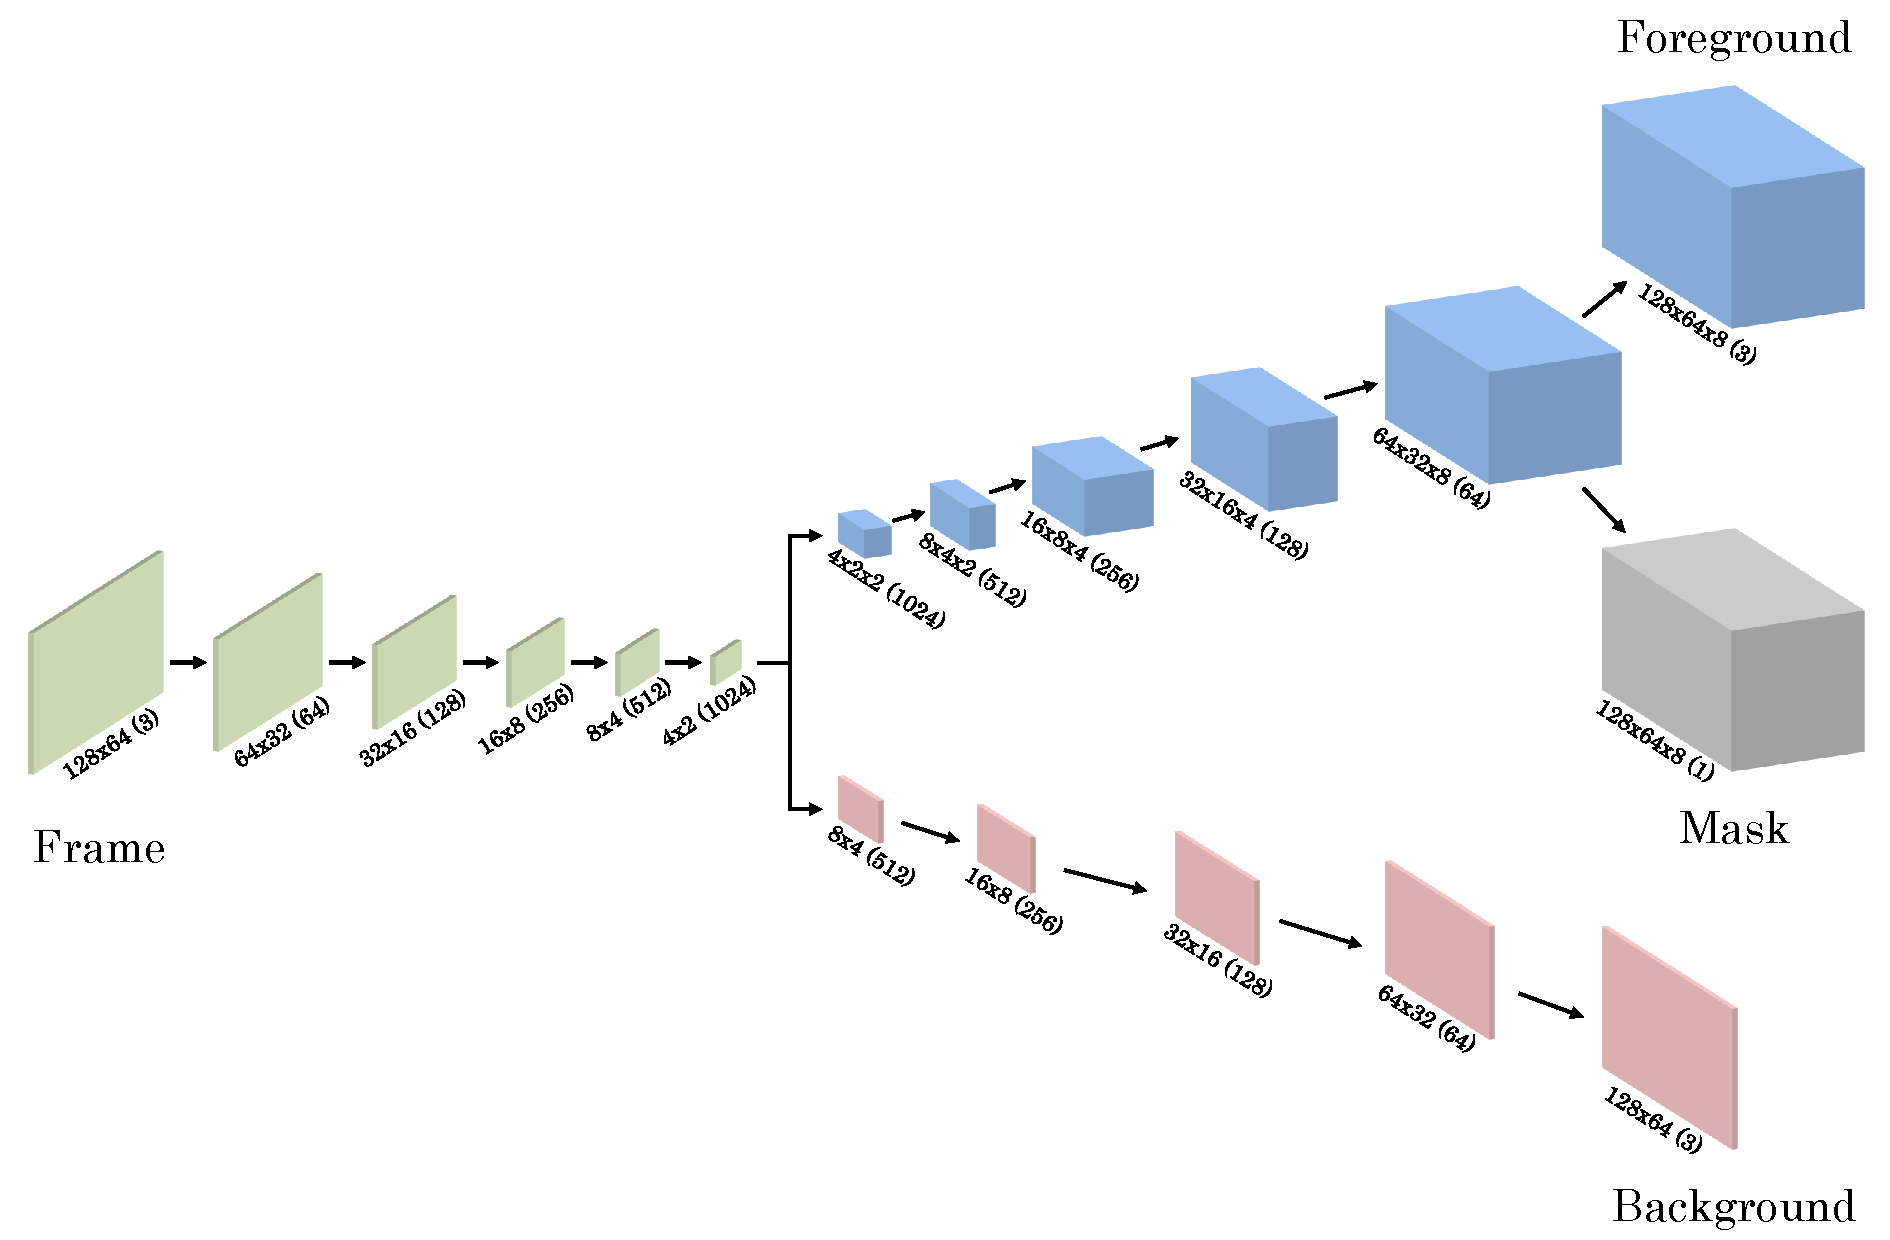
\includegraphics[width=1\textwidth]{graphics/gan/vgan/cvgan_1/cvgan_1.pdf}
  \caption[Adapted video prediction network ($n$ out of $1$ frames).]{Adapted C-VGAN video prediction (generator) network \cite{vondrick2016generating}. Instead of random noise a single frame encoded through strided spatial convolutions to latent space serves as input for the two streams. The rest of the architecture mirrors VGAN, including the combination of foreground, mask, and background to create the generated video output. The number in parentheses is the number of channels.}  
  \label{fig:cvgan_1}
\end{figure}

This minimizes the L1 (Manhattan) distance between the input frame ($x_0$) and the first frame of the respective generated video ($G^0(\cdot)$). $\lambda \in \mathbb{R}$ is a hyperparameter to weight the first frame reconstruction loss with the other two losses. This way, the generator can not simply enter mode collapse, i.e. collapsing different input frames into the same realistic looking output videos. Instead it has to reconstruct the first frame, before learning to generate following frames based on the initial scene. The rest of the generator and discriminator network remain the same.  The resulting model, sometimes called a conditional generative adversarial network for video (C-VGAN) \cite{tulyakov2018mocogan}, was used to extrapolate plausible motions in different scenes. $32$ frames were extrapolated from a single frame beginning that sequence. 

Unfortunately we noticed when inspecting the actual code referenced in the paper by Vondrick et al.\footnote{\url{https://github.com/cvondrick/videogan/blob/master/main_conditional.lua}}, that there were several additional changes done to both the generator and the discriminator without mentioning it anywhere: Not only does the encoder not mirror the background stream --- having only four instead of five convolutional layers, but the number of channels for each convolutional layer was doubled as well. The convolutional filters range from a number of $128$ to $1024$ for the latent space, instead of the expected $64-512$. This also doubled the resulting size of the bottleneck. The rest of the generator was however also altered because of that: Instead of keeping the five layer stack of the two streams, one layer was removed from the background pathway, while the foreground was kept was kept as it was in VGAN. Why these changes were done to the network is not explained anywhere; the version of the code is from the initial commit of that repository. One can assume the widening of the bottleneck and the doubling of the number of filters at every layer were done consciously to avoid the collapse of different inputs to the same generated video. What it does not explain however is the changes for the discriminator. There, the number of convolutional filters was also doubled at every step of the CNN-based classifier. As explained in Section \ref{sec:gans}, this serves to empower the discriminator and prevent the domination of a strengthened generator model. So improving the expressiveness of both models simultaneously is usually the right choice \cite{roth2017stabilizing, zhang2018convergence}.\\

\begin{figure}
	\centering
	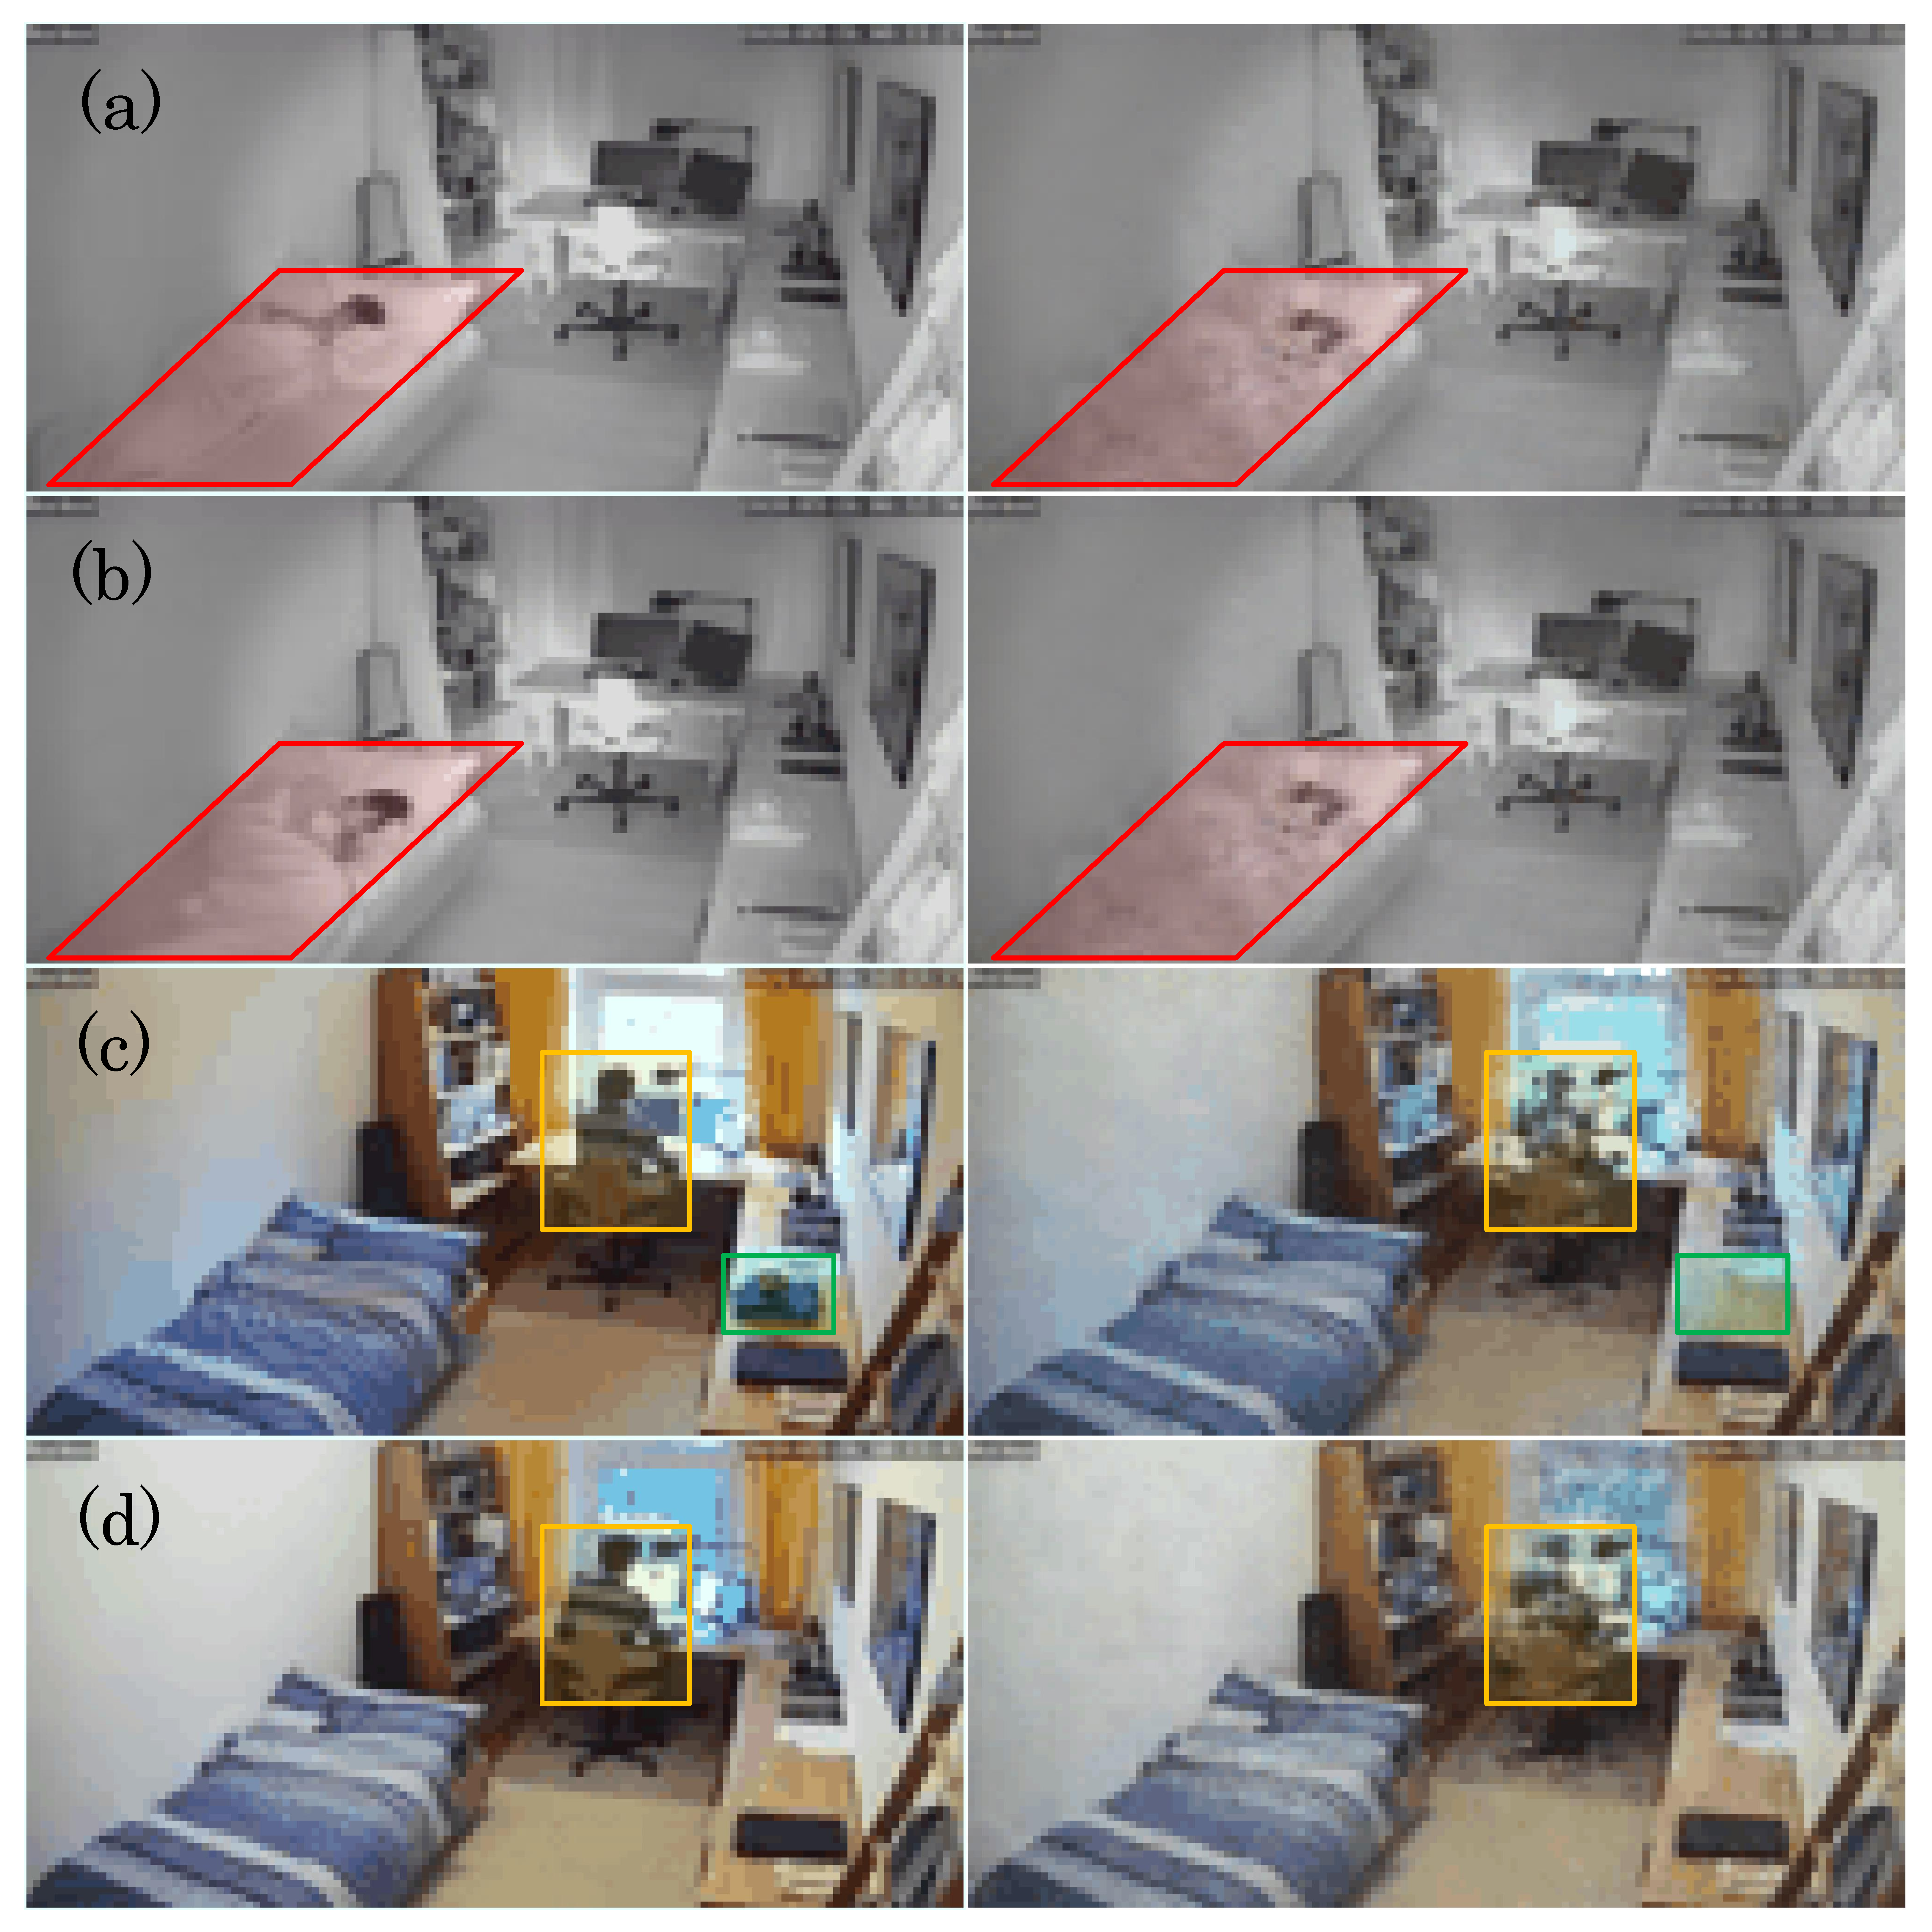
\includegraphics[width=0.6\textwidth]{graphics/eval/cvgan_1/cvgan_1_Collapse.pdf}
  \caption[Comparison between inputs of C-VGAN and their reconstructed outputs.]{First frames that are passed to C-VGAN (left) and the generated first frames (right). Marked in red (a,b) one can see how different object patterns are collapsed into the same pattern during reconstruction. In (c) objects (green) are omitted from the scene entirely. Some object patterns are also not fully reconstructed (yellow), e.g. the person's neck and some of its other features are missing in (d).}
  \label{fig:cvgan_1_out}
\end{figure}

\paragraph{Modifications to C-VGAN}
Due to these ambiguities, when adapting C-VGAN to our data, we first decided to build our interpretation of C-VGAN on our VGAN model described in Section \ref{subsec:vgan_mod} but mix it with the design decisions made in the original C-VGAN code. This results in the generative model depicted in Figure \ref{fig:cvgan_1}: Because our modified models had one additional convolutional layer in each of their streams, the encoder that was attached to our generator has five convolutional layers instead of four. Therefore, the 2D latent space has a size of $4 \times 2$ with $1024$ convolutional filters and both background and foreground upsample from that directly. As the modified VGAN generator, a kernel size of $3$ was used instead of $4$. Because foreground and background stream can directly upsample from the latent space to the next step ($8 \times 4$), doubling the used number of convolutional filters at every step of the stacks, one fractionally-strided convolutional layer was removed from the background. For the foreground stream, the first convolutional layer was instead used to transform the latent code into a 3-dimensional one, using a stride of $2$ along the time axis as in the original C-VGAN. Finally, we kept all of our other modifications to VGAN, such as the weight initialization. The expressiveness of the discriminator was not increased however and it was kept the same.

During our tests with the modified C-VGAN we noticed that even the original discriminator was dominating the modified empowered generator. The empowering of which, by also doubling the number of its convolutional filters as done in the generator, was therefore not necessary. The continued use of the discriminator that was built for VGAN, will be further highlighted in the following section and in Chapter \ref{chap:results}, when we evaluate the different configurations of our final GAN. Other issues we encountered with C-VGAN were similar to the ones Vondrick et al. found. They hint at the bottleneck of the latent space that is still too strong: Forms of mode collapse and the dropping or hallucination (i.e. insertion) of objects were among these. In Figure \ref{fig:cvgan_1_out} one can see the first frames for several different outputs and how the generator model struggles to reconstruct them. Finally, although this model could be integrated into an anomaly detection framework such as IFTM, it is impaired by its very nature: By only using a single frame to predict the future --- not only a single future frame but in our adaptation $7$ frames, the degrees of freedoms for the forecast is too great: While the future may be plausible, it is not likely it will come to pass. In addition, because of our use-case, there is no need to only utilize a single frame as a starting point for forecasting. A continuous stream of video frames is available to the model. Thus in the following section, we adapt C-VGAN to be more constrained during future frame generation.


\subsection{C-VGAN with Spatio-Temporal Input} \label{subsec:vgan_mod_2}

As noted during the modification of C-VGAN and in our use case, the ADS and thus the underlying model as well, have to process frames of the continuous video stream once during the detection phase, one after the other. This is a key difference to the application of VGAN and C-VGAN, that were evaluated using short video clips from Flickr\footnote{\url{www.flickr.com}} \cite{vondrick2016generating}. These clips beside common themes, were usually not directly related to each other, while in our case, the same person appears in many frame windows with similar motion patterns in different contexts. However due to the nature of a single encoder for both generator streams, similar motion and appearance patterns of the same object might be represented differently in the latent space of the generator. This forces the two streams to waste part of their capacity by learning these meaningful features redundantly. This issue was also noticed in later research in video generation \cite{tulyakov2018mocogan, spampinato2018vos, spampinato2019adversarial}, and the solution that was proposed is the further untangling of the two streams in terms of input: Spampinato et al. utilize one traditional latent space for the background stream and a trajectory latent space to ensure spatio-temporal consistence of the foreground \cite{spampinato2019adversarial}, i.e. generating a random latent vector for each of frames that have to be generated (see Section \ref{sec:rel_vgan}). Taking the explicit untangling of the input and transforming VGAN to a next frame prediction model, we propose an extension to C-VGAN to accept spatio-temporal data --- videos, as input. These changes also widen the bottleneck of the generator, which help with the issues that were encountered during the use of C-VGAN.

\begin{figure}
  \centering
  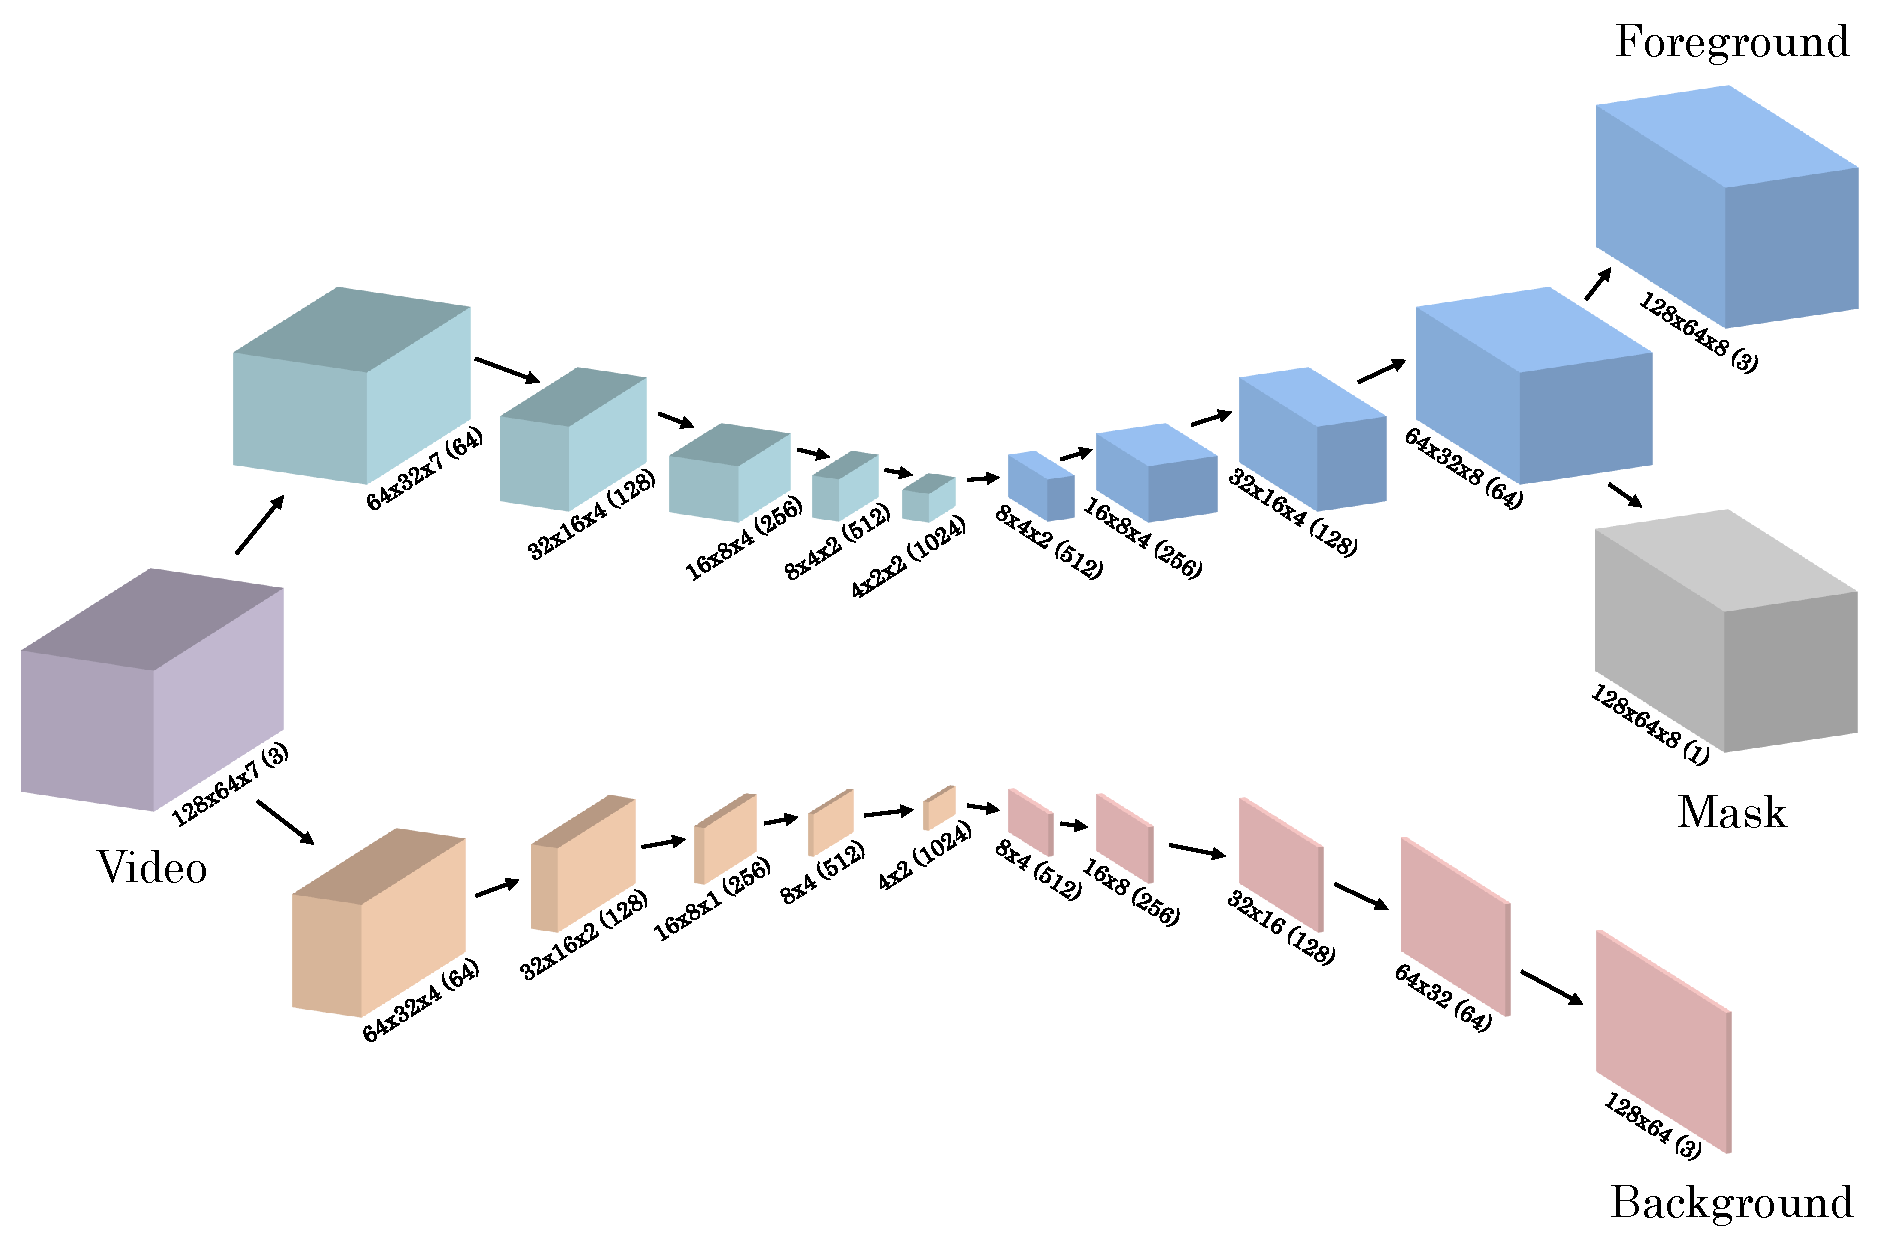
\includegraphics[width=1\textwidth]{graphics/gan/vgan/cvgan_2/cvgan_2.pdf}
  \caption[Next-frame video prediction network.]{Next-frame video prediction (generator) network. Conditional foreground and background stream are further untangled by using different encoders and latent spaces for each of their inputs. Both encoder streams use strided spatio-temporal convolutions, with the background encoder stream falling back to spatial convolutions once the time dimension has been reduced to size 1. The rest of the architecture mirrors VGAN, including the combination of foreground, mask, and background to create the generated video output. The number in parentheses is the number of channels.}
  \label{fig:cvgan_2}
\end{figure}

\begin{table}
	\centering
	\begin{tabular}{ | l | l | l | c | c | c | r !{\makebox[0pt]{$\times$}} r !{\makebox[0pt]{$\times$}} r !{\makebox[0pt]{$\times$}} r |}
	\toprule
	\textbf{\textit{Fg Stream}}			& \textbf{Kernel} 		& \textbf{Stride} 		& \textbf{BN} 	& \textbf{AF} 	& \textbf{Init} & \multicolumn{4}{c |}{\textbf{Output Shape}} \\
	Input 								& $-$  					& $-$  					& $-$  			& $-$  			& $-$ 			& 3 & 128 & 64 & 7		\\
	Conv3D 								& $3 \times 3 \times 3$	& $2 \times 2 \times 1$	& No 			& ReLU 			& He 			& 64 & 64 & 32 & 7		\\
	Conv3D 								& $3 \times 3 \times 3$ & $2 \times 2 \times 2$	& Yes 			& ReLU 			& He 			& 128 & 32 & 16 & 4		\\
	Conv3D 								& $3 \times 3 \times 3$ & $2 \times 2 \times 1$	& Yes 			& ReLU 			& He 			& 256 & 16 & 8 & 4		\\
	Conv3D 								& $3 \times 3 \times 3$ & $2 \times 2 \times 2$	& Yes 			& ReLU 			& He 			& 512 & 8 & 4 & 2		\\
	Conv3D 								& $3 \times 3 \times 3$ & $2 \times 2 \times 1$	& Yes 			& ReLU 			& He 			& 1024 & 4 & 2 & 2		\\
	Conv3DTrans 						& $3 \times 3 \times 3$ & $2 \times 2 \times 1$	& Yes 			& ReLU 			& He 			& 512 & 8 & 4 & 2		\\
	Conv3DTrans 						& $3 \times 3 \times 3$ & $2 \times 2 \times 2$	& Yes 			& ReLU 			& He 			& 256 & 16 & 8 & 4		\\
	Conv3DTrans 						& $3 \times 3 \times 3$ & $2 \times 2 \times 1$	& Yes 			& ReLU 			& He 			& 128 & 32 & 16 & 4		\\
	Conv3DTrans 						& $3 \times 3 \times 3$ & $2 \times 2 \times 2$	& Yes 			& ReLU 			& He 			& 64 & 64 & 32 & 8		\\
	\midrule
	\textbf{\textit{Foreground ($f$)}} 	& \textbf{Kernel} 		& \textbf{Stride} 		& \textbf{BN} 	& \textbf{AF} 	& \textbf{Init} & \multicolumn{4}{c |}{\textbf{Output Shape}} \\
	Conv3DTrans 						& $3 \times 3 \times 3$	& $2 \times 2 \times 1$	& No 			& Tanh 			& Glorot 		& 3 & 128 & 64 & 8 	\\
	\midrule
	\textbf{\textit{Mask ($m$)}} 		& \textbf{Kernel} 		& \textbf{Stride} 		& \textbf{BN} 	& \textbf{AF} 	& \textbf{Init} & \multicolumn{4}{c |}{\textbf{Output Shape}} \\
	Conv3DTrans 						& $3 \times 3 \times 3$	& $2 \times 2 \times 1$ & No 			& Sigmoid 		& Glorot 		& 1 & 128 & 64 & 8 	\\
	TileTensor($3$)						& $-$  					& $-$  					& $-$  			& $-$  			& $-$ 			& 3 & 128 & 64 & 8 	\\
	\midrule
	\textbf{\textit{Bkg Stream ($b$)}} 	& \textbf{Kernel} 		& \textbf{Stride} 		& \textbf{BN} 	& \textbf{AF} 	& \textbf{Init} & \multicolumn{4}{c |}{\textbf{Output Shape}} \\
	Input 								& $-$  					& $-$  					& $-$  			& $-$  			& $-$ 			& 3 & 128 & 64 & 7		\\
	Conv3D 								& $3 \times 3 \times 3$	& $2 \times 2 \times 2$	& No 			& ReLU 			& He 			& 64 & 64 & 32 & 4		\\
	Conv3D 								& $3 \times 3 \times 3$	& $2 \times 2 \times 2$	& Yes 			& ReLU 			& He 			& 128 & 32 & 16 & 2		\\
	Conv3D 								& $3 \times 3 \times 3$	& $2 \times 2 \times 2$	& Yes 			& ReLU 			& He 			& 256 & 16 & 8 & 1		\\
	Conv2D 								& $3 \times 3$			& $2 \times 2$			& Yes 			& ReLU 			& He 			& 512 & 8 & \multicolumn{1}{ r }{4}	&	\\
	Conv2D 								& $3 \times 3$			& $2 \times 2$			& Yes 			& ReLU 			& He 			& 1024 & 4 & \multicolumn{1}{ r }{2} &	\\
	Conv2DTrans 						& $3 \times 3$			& $2 \times 2$			& Yes 			& ReLU 			& He 			& 512 & 8 & \multicolumn{1}{ r }{4} &	\\
	Conv2DTrans 						& $3 \times 3$			& $2 \times 2$			& Yes 			& ReLU 			& He 			& 256 & 16 & \multicolumn{1}{ r }{8} &	\\
	Conv2DTrans 						& $3 \times 3$			& $2 \times 2$			& Yes 			& ReLU 			& He 			& 128 & 32 & \multicolumn{1}{ r }{16} &	\\
	Conv2DTrans 						& $3 \times 3$			& $2 \times 2$			& Yes 			& ReLU 			& He 			& 64 & 64 & \multicolumn{1}{ r }{32} &	\\
	Conv2DTrans 						& $3 \times 3$			& $2 \times 2$			& No 			& Tanh 			& Glorot 		& 3 & 128 & \multicolumn{1}{ r }{64} &	\\
	RepeatTensor($8$) 					& $-$  					& $-$  					& $-$  			& $-$  			& $-$  			& 3 & 128 & 64 & 8 \\
	\bottomrule
	\end{tabular}
	\caption[Architecture of the generator.]{Architecture of the generator: \textit{Fg Stream} lists the layers included in the foreground stream of the model, which is then split into the \textit{Foreground} and its spatio-temporal \textit{Mask}. \textit{Bkg Stream} contains the respective layers of the background stream. The combination of the three tensors is done as described in Equation \ref{eq:vgan}. Note that \textit{Conv3D} stands for strided spatio-temporal convolution, while \textit{Conv3DTrans} stands for its fractionally-strided counterpart. The same is the case for the spatial convolutions used in the background stream. The usage of batch normalization (\textit{BN}), an activation function (\textit{AF}), and the initializer for the kernel weights (\textit{Init}) is also listed per layer.}
	\label{tab:cvgan_arch_g}
\end{table}

\paragraph{Generator}
First for the generator, the single encoder that was attached to the front of the generator in the original C-VGAN is replaced with two separate ones for each stream, which results in the usage of two separate latent spaces. For the encoder that has to create the trajectory latent code to model object patterns for the foreground, a spatio-temporal CNN is attached. Now, instead of a single frame, a sequence of frames are passed to the encoder as input. As with the foreground afterward, convolutional filters range from $64$ to $1024$, using a kernel size of $3$ and a stride of $2$, except for the time axis. The time dimension is again only halved every other step. As shown in Figure \ref{fig:cvgan_2} and described in detail in Table \ref{tab:cvgan_arch_g}, $7$ input frames are passed to the CNN encoder and due to padding during the application of the convolutional filters, the time dimension returns to an even size of $4$ after the second layer. The resulting bottleneck and the trajectory latent space has twice the size of the one in C-VGAN for the foreground alone ($4 \times 2 \times 2$). This is necessary because instead of a preset for a scene for which a video needs to be generated, the information of appearance and motion patterns across multiple frames has to be stored in latent space. Lastly, the first fractionally-strided convolutional layer that was exclusively used in C-VGAN to transform the former spatial latent code into a a spatio-temporal one, is removed.

For the background stream, the encoder is also spatio-temporal at the beginning. Although the background is a static frame that is generated using 2D de-convolutions, the input video --- a space time cuboid, can not be simply flattened or otherwise modified. For example, when using a single frame instead of all $7$ input frames, this results in the loss of information: Static objects in the background might be obscured by dynamic ones. The former objects are thus impossible to be generated by the background stream, because they did not appear in its encoded latent space. These static objects would need to be generated by the foreground instead, that still has the necessary information. But this is not desired. Ideally the background stream is able to generate the entire static part of the scene and the spatio-temporal mask of the foreground stream can show or remove static objects across the frame sequence. Therefore, the first three layers of the background encoder stream are 3D convolutions with a constant stride of $2$ for the convolutional window, so the tensor can be reshaped into a 2-dimensional one (the size of the time dimension is $1$). Afterwards the downsampling to latent code continues using spatial convolutions. This quick reduction of spatio-temporal information in the background encoder stream forces the background to focus on static objects and scenery, while the foreground learns the motion dynamics of non-static objects.

\paragraph{Value Function} \label{par:vgan_mod_2_vfn}
In addition, the loss function during training has to be again extended to account for the reconstruction of all the frames that serve as the input for the generator, as seen in Equation \ref{eq:cvgan_2}. In the case of the displayed generator, $7$ out of $8$ frames ($x_{0;6}$) have to be reconstructed, while the next frame of that sequence has to be extrapolated from them.

\begin{equation} \label{eq:cvgan_2}
\begin{aligned}
\min_G \max_D V(D,G) = & \mathbb{E}_{x \sim p_x(x)}[\log D(x)] + \mathbb{E}_{x_{0;6} \sim p_{x_{0;6}}(x_{0;6})}[\log(1 - D(G(x_{0;6})))] \\
+ & \mathbb{E}_{x_{0;6} \sim p_{x_{0;6}}(x_{0;6})}[\lambda \cdot \|(x_{0;6} - G^{0;6}(x_{0;6}))\|_1]
\end{aligned}
\end{equation}

\begin{table}
	\centering
	\begin{tabular}{ | l | l | l | l | c | c | c | r !{\makebox[0pt]{$\times$}} r !{\makebox[0pt]{$\times$}} r !{\makebox[0pt]{$\times$}} r |}
	\toprule
	\textbf{\textit{Disc.}}	& \textbf{Kernel} 		& \textbf{Stride} 		& \textbf{BN} & \textbf{AF} & \textbf{DO}  	& \textbf{Init} & \multicolumn{4}{c |}{\textbf{Output Shape}} \\
	\midrule
	Input         			& $-$         			& $-$         			& $-$         & $-$ 		& $-$           	& $-$ 			& 3 & 128 & 64 & 8						\\
	Conv3D        			& $3 \times 3 \times 3$ & $2 \times 2 \times 1$ & No          & LReLU		& $dr$	 		& He			& $cf$ & 64 & 32 & 8					\\
	Conv3D        			& $3 \times 3 \times 3$ & $2 \times 2 \times 2$ & Yes         & LReLU		& $dr$	 		& He			& $(2 \cdot cf)$ & 32 & 16 & 4			\\
	Conv3D        			& $3 \times 3 \times 3$ & $2 \times 2 \times 1$ & Yes         & LReLU		& $dr$	 		& He			& $(4 \cdot cf)$ & 16 & 8 & 4			\\
	Conv3D        			& $3 \times 3 \times 3$ & $2 \times 2 \times 2$ & Yes         & LReLU		& $dr$	 		& He			& $(8 \cdot cf)$ & 8 & 4 & 2			\\
	Conv3D        			& $3 \times 3 \times 3$ & $2 \times 2 \times 1$ & Yes         & LReLU		& $dr$	 		& He			& $(16 \cdot cf)$ & 4 & 2 & 2			\\
	Dense         			& $-$         			& $-$         			& $-$         & $-$         & $-$	 		& Glorot 		& \multicolumn{1}{ r }{1} & \multicolumn{1}{ r }{} & \multicolumn{1}{ r }{} &			\\
	\bottomrule
	\end{tabular}
	\caption[Architecture of the discriminator.]{Architecture of the discriminator: As a one-stream CNN, a video is downsampled using strided spatio-temporal convolutions (\textit{Conv3D}) before a single fully connected neuron (\textit{Dense}) gives the binary classification result. The activation function (\textit{AF}) \textit{LReLU} stands for Leaky ReLU and its negative slope coefficient is $\alpha = 0.3$. Batch normalization (\textit{BN}), activation function, and then dropout (\textit{DO}) with a rate of $dr$ is applied to every convolutional layer, in order. The first dimension of each layers output --- the number of channels, i.e. convolutional filters, can be tuned using the $cf$ hyperparameter.}
	\label{tab:cvgan_arch_d}
\end{table}

\paragraph{Discriminator}
Yet this kind of reconstruction loss term comes at a disadvantage: As explained in Section \ref{sec:gans}, the strength of GANs lie in the generator's inability to directly learn from real examples, while the discriminator gives it hints how to fake outputs. This ideally (if there is no mode collapse) allows the generator to generalize well. For example generating similar motion dynamics of objects in video, without ever seeing that kind of motion during training. On the other hand, limiting the degrees of freedom for the generator is necessary due to use video generation for forecasting. This changes the goal of the discriminator in some sense, although the loss term has not been altered explicitly in this manner: $D$ still needs to distinguish real from synthetic videos, but it will quickly learn to ignore the first $7$ out of $8$ synthetic frames for the purpose of discrimination. These frames will appear real because they were reconstructed from real input and the generator learns this through the modified loss term. Now the deciding factor for $D$ is how well the extrapolation from the input frame sequence to the last frame was done. Thus, although the generator has increased in capacity, $D$'s job is actually easier now. This phenomenon is noticed during evaluation in Section \ref{subsec:cvgan_results}, where $D$ overpowers $G$ in a matter of a few epochs. 

Consequently, several options to impair $D$ are introduced: While keeping the overall architecture of the discriminator that was used through the different modification stages, the first impairment parameter is the number of filters for the first convolutional layer and its subsequent layers respectively; following the DCGAN architecture the amount of convolutional filters is doubled with every next convolutional layer. The default value for this hyperparameter ($cf$) is $32$, as that was the configuration that was used during the VGAN and C-VGAN adaptations. Second, regularization layers in the form of dropout layers are added after every layer and its respective activation. The rate of the input units the layers set to $0$ is another set of hyperparameters (default is $dr=0$, no dropout). Further impairment was not required --- the negative slope coefficient ($\alpha=0.3$) of the Leaky ReLU activations used in the discriminator instead of typical ReLU, was also not tuned. An improvement of the generator was also not feasible due to its already high complexity and number of parameters that have to be optimized already. A summary of the model and its parameters can be seen in Table \ref{tab:cvgan_arch_d}.



% Anomaly Detection for Video using IFTM
\section{Anomaly Detection for Video using IFTM} \label{sec:vad}

\begin{figure}
	\centering
	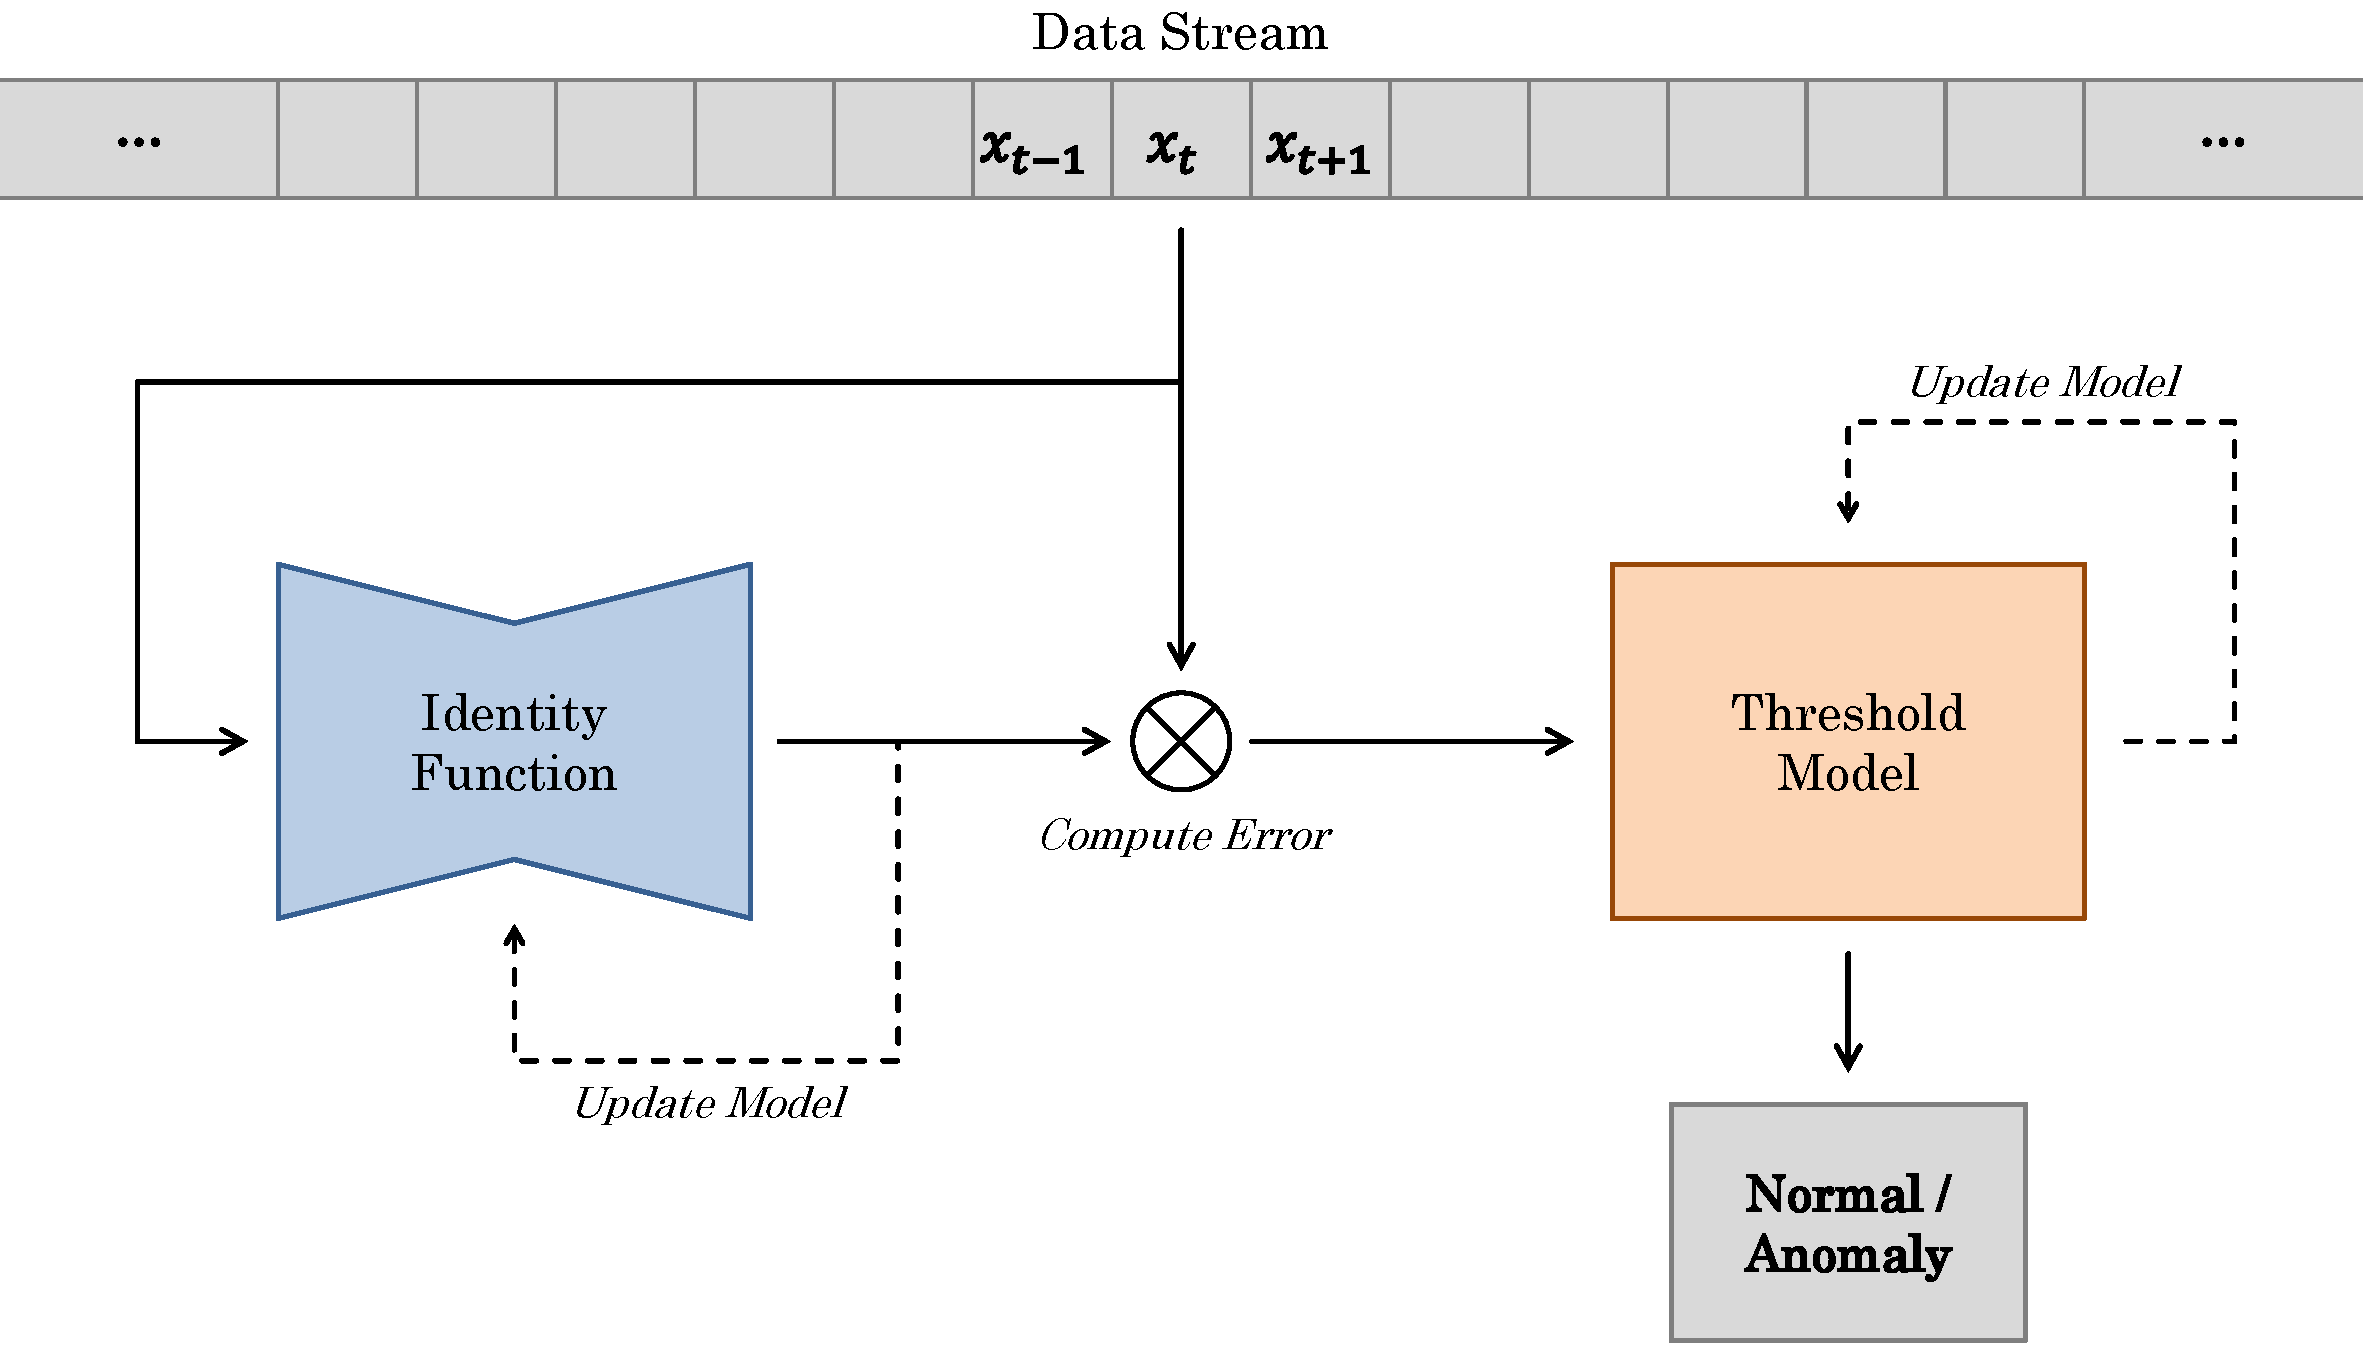
\includegraphics[width=1\textwidth]{graphics/iftm/iftmOriginal/iftmOriginal.pdf}
  \caption[IFTM framework.]{IFTM operating on a data stream. Both identity function and threshold model are trained while making predictions at runtime.}
  \label{fig:iftm}
\end{figure}

As explained in detail in Section \ref{sec:anomaly_detection}, many ADS give the administrator a prediction per event or observation, ranging from $0$ to $1$. This anomaly score describes the model's grade of certainty that a data point is truly an anomaly. Applying a threshold to map this score to a binary result is crucial, but as explained, it is often required that experts set a static threshold for what they consider anomalous. Schmidt et al. solve this challenge through IFTM \cite{schmidt2018iftm}, a framework that combines two components as depicted in Figure \ref{fig:iftm}: The identify function (IF)\nomenclature{IF}{Identity function} serves as the underlying model that computes the anomaly score: Trained in unsupervised manner, the IF is supposed to model the properties of the normality of the data stream, while being unable to model anomalous observations. As the name suggests, Schmidt et al. use the identity function $s: X \rightarrow X$ with $x \in X$ being a single observation in the stream. $s$ is approximated by using the observations witnessed in the past in online fashion. And because it is assumed that the stream is mostly normal in nature, $s$ is able to reconstruct normal observations more easily. The reconstruction of $s(x)=x^{\prime}$ when $x$ is anomalous however should have a higher reconstruction error $\Delta$, because the model is unable to model its properties:

\begin{equation} \label{eq:recon}
\Delta(x) = ||x-s(x)||_2
\end{equation}

For the IF, any kind of model that supports reconstruction can be used, including models from the field of deeplearning. Reconstruction can also be replaced by a forecasting model, as Schmidt et al. suggest. Instead of computing the reconstruction shown in Equation \ref{eq:recon} and minimizing it during training, the model instead has to learn to predict the next observation of the stream, $x_t$. As shown in Equation \ref{eq:forc}, the prediction and therefore the prediction error this time is done on a number of past observations. Because IFTM is abstract by design, the underlying forecasting model could be anything and therefore could use the past in different ways. For example, one could use a type of recurrent neural network (RNN)\nomenclature{RNN}{Recurrent neural network}, such as long short-term memory (LSTM)\nomenclature{LSTM}{Long short-term memory} units, that dynamically learns to ignore certain inputs or forget past ones \cite{hochreiter1997long}.

\begin{equation} \label{eq:forc}
\Delta(x_{t}) = ||x_{t}-s(x_{0;t-1})||_2
\end{equation}

Due to the IF being ideally trained in online manner --- it should be able to adapt to new contexts and normal properties of the data stream, the meaning of a specific anomaly score can also change over time. But one still has make the binary discrimination at the moment the observation occurs. Therefore, Schmidt et al. propose a second model that represents the threshold $T$, that is applied to $\Delta(x)$, the threshold model (TM)\nomenclature{TM}{Threshold model}. If the reconstruction or forecasting error is greater than $T$, it is considered an anomaly. As $s$ adapts to the data stream, $T$ has to adapt with it and is therefore also trained in an unsupervised online manner. Assuming $\Delta$ is normally distributed, $T$ for a given data stream can be defined with the following:

\begin{equation} \label{eq:tm}
T = \mu(\Delta) + \sigma(\Delta)
\end{equation}

\begin{figure}
	\centering
	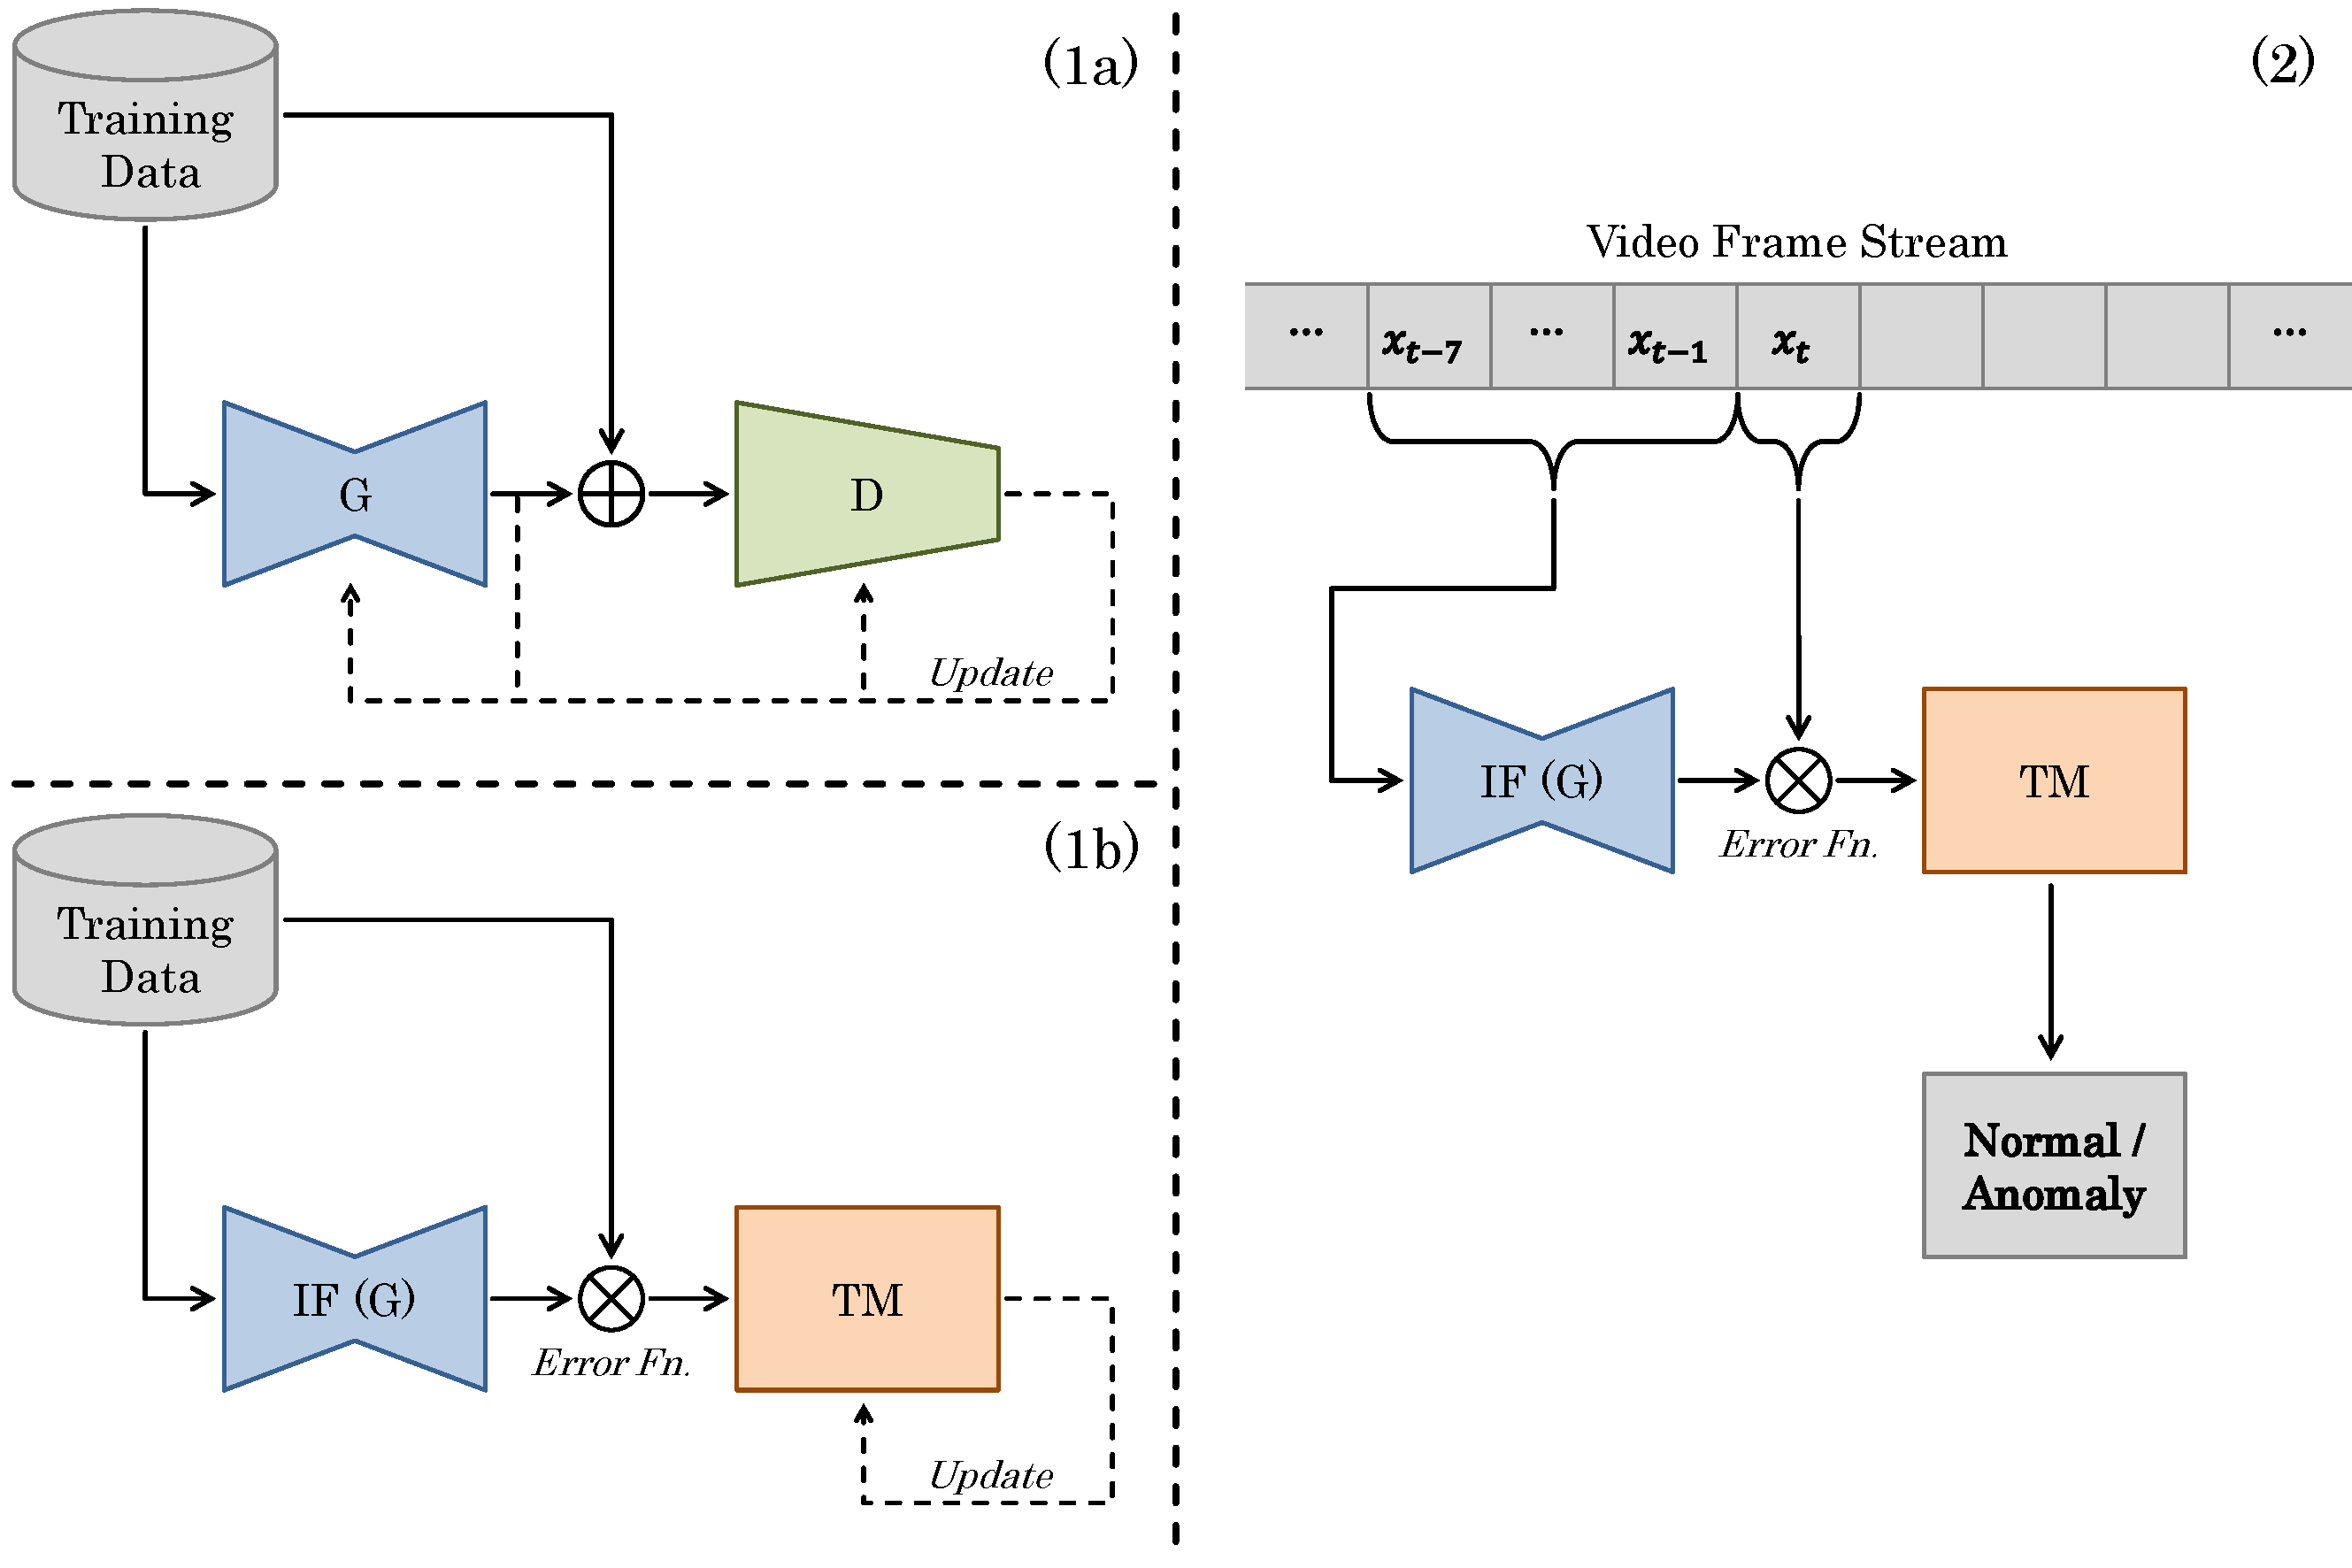
\includegraphics[width=1\textwidth]{graphics/iftm/iftmModified/iftmModified.pdf}
  \caption[IFTM framework adapted for video generation forecasting.]{IFTM framework adapted for video generation forecasting, by splitting training and prediction into separate phases: (1a) features the training of the C-VGAN next-frame video prediction generator network (\textit{G}) and its discriminator (\textit{D}), following the GAN training loop. In (1b) the threshold model (\textit{TM}) is trained using the training data and the trained generator model as identity function (\textit{IF}). In the second phase (2), IFTM makes next-frame video prediction on the stream, labeling frames as either normal or anomalous.}
  \label{fig:iftm_video}
\end{figure}

How the mean ($\mu$) and the standard deviation ($\sigma$) is computed depends on the use case. First, one can compute these two iteratively over the entire data stream online. This kind of cumulative aggregation of two values is not stable however with longer periods of time because the past will dominate $T$ as newer values have less weight assuming an infinite stream. Alternatives present themselves in the form of sliding window aggregations and moving averages in which older data points of the stream are discarded from the distribution. One can also compute $T$ using other techniques but for the sake of our approach, it is assumed that the reconstruction error follows a normal distribution and $T$ can be defined using the equation above.

\paragraph{IFTM with Video Generation Forecasting}
Assuming that a video generation model trained on mostly normal data will model the normal properties of video while being unable to find a representation for anomalous video frames, we propose an integration of our adapted C-VGAN for next-frame video forecasting into IFTM to perform VAD. This requires some modifications to IFTM: First for C-VGAN the reconstruction of past frames is done using the Manhattan (L1) distance and not the Euclidean (L2) distance, as described in the previous section. This also indirectly defines the properties of the forecast frame. So when computing the prediction error for a forecast video frame the L1 metric is utilized. Also, our adapted C-VGAN next-frame prediction network in the configuration presented uses a fixed number of past frames ($7$) to predict the next one. This results in the following adjusted prediction error function:

\begin{equation} \label{eq:forc_2}
\Delta(x_{t}) = ||x_{t}-s(x_{t-7;t-1})||_1
\end{equation}

Second, as explained in Section \ref{sec:gans}, training of any GAN is never done online but done on the entire training data set available. Splitting the data into smaller equal-sized mini-batches, the two models are optimized in min-max fashion until a somewhat stable convergence of their losses is achieved and satisfactory synthetic values are generated. This can require dozens if not hundreds of iterations --- also called epochs, over the entire data set. Because it is not feasible to do the training of the GAN online, neither the TM is trained online. Thus, both forecasting model and TM operate as displayed in Figure \ref{fig:iftm_video}: During the (offline) training phase, the GAN is first trained in usual manner until convergence is achieved. Then, the entire training set is re-run on the generator model to compute the prediction errors and the resulting mean and standard deviation of the errors over the training set. Then in the detection phase, when running on the unknown data stream, forecasting, computation of the error, and the application of $T$ is done online. Note that when training IFTM this way, the framework will no longer have the ability to react to context shifts over time. The underlying prediction model has to learn all properties that normal data can have during the offline training phase, taken it has enough capacity to learn all these features. This does not matter for our our evaluation of IFTM for video though, because the data comes from a single camera source over a variety of days and the labeled evaluation data is from the same time frame. There is no noticeable context shift over that time span. How the data sets were created, labeled, and how they are structured will be explained in the following section.



% Dataset
\section{Data Set} \label{sec:dataset}

In this section, the large-scale data set for VAD evaluation, that was already touched upon in the use case in Section \ref{sec:use_case}, is presented. We provide insight into how the data set is structured and what properties it has. For the labeled video data, an analysis based on the kind of normal and anomalous frames in it is done. This includes statistics regarding the balance of the two classes. Lastly, the different steps that were taking during preprocessing of the video files are mentioned and the reason why they were taken are explained.


% Creation of Dataset, Underlying Structure
\subsection{Properties} \label{subsec:dataset_properties}

To create a large quantity of video data for anomaly detection using video generation, a camera was positioned in a home office room to monitor it over several days. Capturing the video with a resolution of $640 \times 352$ and varying frame rate of $2.5$ to $5$, the view is static; in position, viewing angle, direction, and field of view. During the night, the fps is reduced by the camera automatically due to switching to a grayscale night vision mode. In addition, a timestamp containing the date and the time is in the top right corner of every video frame.

\begin{figure}
	\centering
	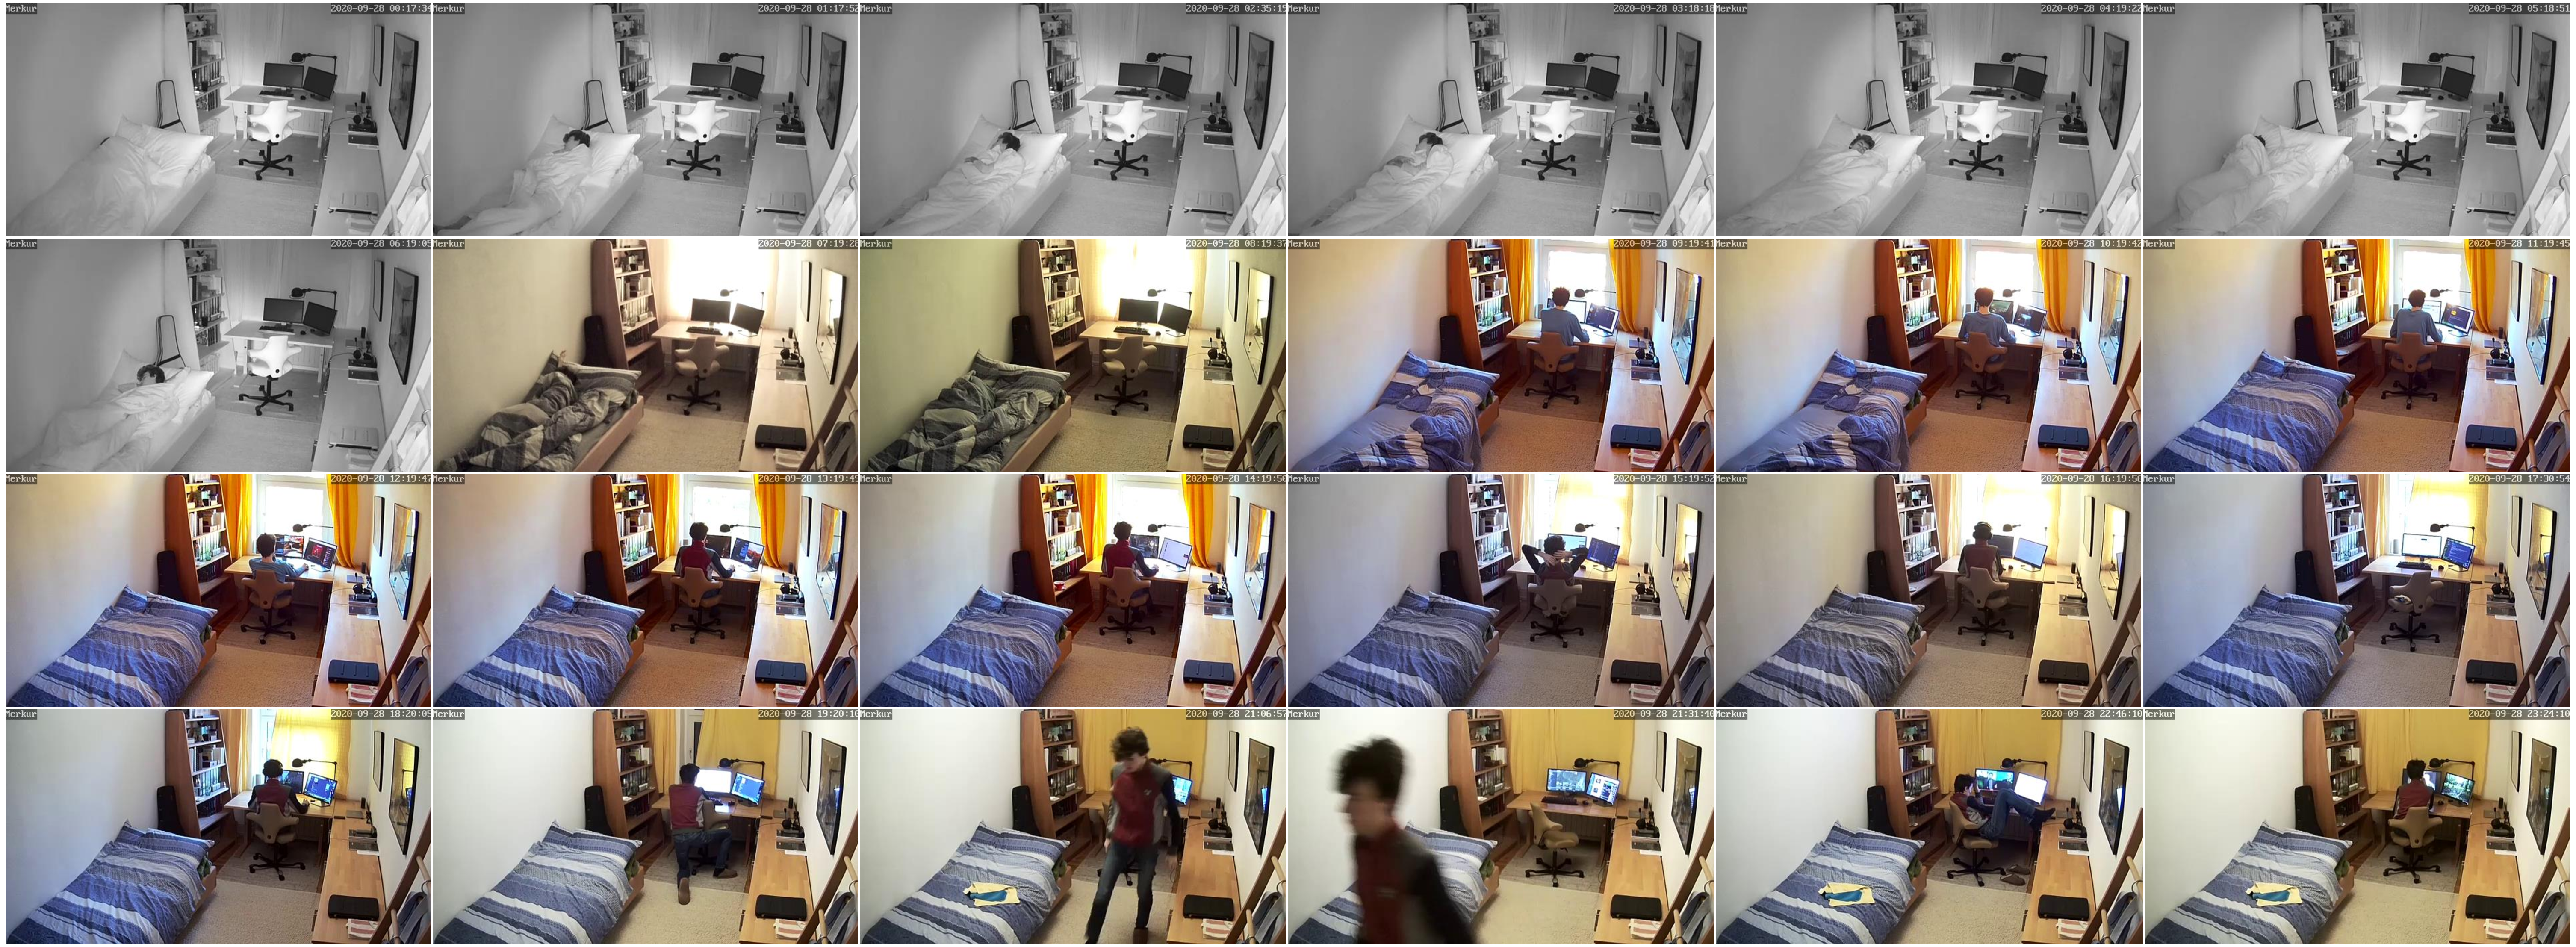
\includegraphics[width=1\textwidth]{graphics/cctv/oneDay/oneDay.pdf}
  \caption[Monitored room during different hours of the day]{Monitored room during the different hours of one of the captured days.}
  \label{fig:room_frames}
\end{figure}

\paragraph{Training Data}
For collecting the unlabeled but assuming mostly normal video data set, monitoring was done atleast for a day to create one part of the data set, generating 24 one hour long videos (MP4 format). Furthermore, capturing was done in bulk, five days each during September and November of 2020, respectively. In Figure \ref{fig:room_frames} frames of each of the 24 hours of one of the monitored days are shown. As one can see, the scenery does not change much overall --- the person usually works at the desk and sleeps in the bed behind them during the night when the light is turned off. Although the person moves around, enters and leaves the room from time to time, the video is often static. This offers any VAD an additional challenge, because the video is unfiltered: Depending how the data set is used during training, a model has to refrain from collapsing into a naive motion detector that considers any kind of movement and abrupt change as anomalous behavior. It has to learn to identify ``idle`` intervals in the video, in which for example the person is sleeping or the room is empty for several hours in a row, and quickly understand the normal contents of such, while also being able to recognize normal motion patterns of objects as for what they are. Differentiating these from anomalous ones is the challenge. Furthermore, the clothing of the person in the room does usually only change twice for a single day. When getting out of bed the clothing changes to day clothes until night, where they switch back to pajamas. Both sets of clothing are not constant across different days however --- the person is not wearing the same kind of clothes every day, so any model should learn to ignore these features and not directly learn them. Else frames in which the person wears unknown clothing will be more likely to be considered anomalous. 

Motion dynamics alone are not the only events of interest to a VAD for our data set: The scenery changes dynamically over the day, as shown in the figure, and this adds lots of contextual information to the scene: For example, during the day, the curtains are open and the person either walks around the room or sits at their desk. As the lighting in the morning increase, at one point the grayscale image switches to the colored view due to the camera adjusting to day-mode. In the evening, the curtains are closed when it gets darker outside, but as long as the light is on, the person still is active in the room. This changes when the light is turned off, as the monitored person goes to bed. This part of the information that has to be extracted is periodic in nature due to the 24-hour cycle and a VAD should be able to model this periodic rhythm. 

The motion patterns of objects are also determined on the context: Lying still in bed is considered normal during the night, but an unusual behavior during the day. Lying on the floor or on the cupboard is also very anomalous no matter the circumstances. But, the line between the two classes become blurry, when there are rare but normal motion patterns that do not appear often during the day. Sitting on the bed for some minutes or standing around in the room, should be considered normal behavior. But due to their rarity, a VAD that has to forget anomalous observations encountered during training to ensure it only contains the normal features of the video, might forget these rare events as well, if it is unable to model similar motion dynamics in the right contexts appropriately.

\paragraph{Evaluation Data}
When building the labeled evaluation set, monitoring was fixed to a single hour. To inject a variety of anomalies into that hour, events were created in quick succession. An event in this case describes a subset of the stream of frames that are somehow related to each other. An event can either be considered normal or anomalous. For example, when standing up and walking through the room, in the video there is a number of frames that contain this event and these frames would each be labeled as normal ones. The events generated range from a second to several minutes, thus being 5 frames to a few thousand frames long. As this set is one hour long, it contains $\sim 18,000$ frames when using a stabilized frame rate (see the next section regarding preprocessing). 

\begin{table}
	\centering
	\begin{tabular}{ | l | c | c | p{9.5cm} |}
	\toprule
	\textbf{Frames} & \textbf{MD} & \textbf{Lights} & \textbf{Normal Event Description} \\
	\midrule
	$00001 - 01557$ & Yes & On & Working at desk, before standing up, leaving room. \\
	$01558 - 01876$ & No  & On & Room left empty. Computer display turned on. \\
	$01877 - 02389$ & Yes & On & Entering the room, walking around. \\
	$02743 - 02831$ & Yes & On & Working at the desk without sitting down. \\
	$03270 - 03666$ & Yes & On & Turning off displays, leaving/entering room. \\
	$03667 - 03672$ & Yes & On & Sitting down at desk. \\
	$04170 - 05420$ & Yes & On & Person turning on displays, then working. \\
	$06861 - 07337$ & Yes & On & Walking around, miscellaneous interactions with room, and leaving/entering room multiple times. \\
	$07338 - 08109$ & Yes & On & Person sitting down at desk, before getting up again, and then leaving room. \\
	$09720 - 09775$ & No  & Off  & Room empty. \\
	$09776 - 10249$ & Yes & Off  & Person entering room, going to bed, and then sleeping. \\
	$10371 - 10509$ & No  & Off  & Room empty. \\
	$10537 - 10608$ & Yes & On 	 & Person walking around, interacting with objects. \\
	$10729 - 11305$ & No  & Off  & Sleeping person in bed. \\
	$11460 - 11924$ & Yes & Off  & Person returning to bed, sleeping. \\
	$11925 - 11970$ & Yes & On   & Person getting up from bed, leaving room. \\
	$12019 - 13959$ & Yes & On   & Working at desk, sometimes getting up, walking around. \\
	$14139 - 14269$ & Yes & On   & Person walking around room before leaving room. \\
	$14270 - 15641$ & No  & On   & Room empty. \\
	$15642 - 16890$ & Yes & On   & Person entering room with different clothing, working, and walking around. \\
	$16893 - 16896$ & No  & On & Room empty. \\
	$17165 - 17168$ & Yes & On & Person leaving room. \\
	$17429 - 18066$ & Yes & Off  & Person returning to bed, sleeping. \\
	\bottomrule
	\end{tabular}
	\caption[Normal events in the evaluation data set.]{Normal events in the evaluation data set sorted by the \textit{Frames} in which they occur. Some events take place while the room is lit (\textit{Lights}) others while the lights are turned off. Not every event has to contain motion dynamics (\textit{MD}); sometimes the room is empty or the person is not moving at all.}
	\label{tab:dataset_normal}
\end{table}

First, for the $5,517$ normal frames, displayed in Table \ref{tab:dataset_normal}, it is to note that that the evaluation data set was created during the evening while it was dark outside. This was done due to the need of artificial light and the closed curtains, which allows us to create many different events. During a normal evening in the home office, the monitored person usually works at the desk, sometimes paces through and out of the room, until eventually going to bed when the lights are turned off. The created normal events mirror that, but with variations to the training data set, e.g. the clothing the person is wearing is different and switches during the evaluation video. In addition, the density of events containing motion dynamics is also higher, to cover the different object patterns that occur over the entire training data set during the evenings and to challenge any VAD model that collapses into a motion detector, labeling every motion pattern as anomalous. This results in some events that usually only appear once during the evening to appear multiple times, while some of them are cut short or left out entirely. For example, it is impossible to have an entire sleep cycle in a labeled data set due to the length of that event that also has little motion dynamics in it, which would also imbalance and skew with the results.

\begin{table}
	\centering
	\begin{tabular}{ | l | c | p{11cm} |}
	\toprule
	\textbf{Frames} & \textbf{Lights} & \textbf{Non-Contextually Anomalous Event Description} \\
	\midrule
	$03136 - 03269$ & On & Person sitting on the edge of the bed, without getting up. \\
	$03673 - 04169$ & On & Person pretending to work at desk, without turning displays on. \\
	$05421 - 05810$ & On & Person moving with chair to middle of room. \\
	$05811 - 05917$ & On & Standing up, leaving chair in middle of room. \\
	$05918 - 06352$ & On & Person kneeling down at desk, chair not at desk. \\
	$06353 - 06440$ & On & Person pacing through room, chair not returned to desk.  \\
	$06441 - 06468$ & On & Pushing chair out of the frame. \\
	$06469 - 06776$ & On & Climbing from chair onto low-board, jumping down from it. \\
	$06777 - 06828$ & On & Person running around room erratically. \\
	$06829 - 06860$ & On & Person moving chair back to desk. \\
	$08110 - 08115$ & $-$ & Turning off lights. \\
	$10510 - 10536$ & $-$ & Turning on lights. \\
	$10696 - 10722$ & $-$ & Turning off lights. \\
	$11971 - 12000$ & $-$ & Turning on lights. \\
	$12001 - 12018$ & On & Pretending to work at desk, without turning displays on. \\
	$17096 - 17164$ & On & Person standing up, moving around erratically. \\
	$17169 - 17218$ & $-$ & Turning off lights. \\
	\bottomrule
	\end{tabular}
	\caption[Non-contextual anomalies in the evaluation data set.]{Non-contextual anomalies in the evaluation data set aggregated by event and their \textit{Frames} in which they occur. All of these either occur when the \textit{Lights} are turned on, or when the lighting of the room changes.}
	\label{tab:dataset_nc_anomaly}
\end{table}

On the other hand for the anomalous events that range a total of $12,549$ frames, a different approach to generate the events was attempted. As explained in Section \ref{subsec:anomaly_types}, in which the three types of anomalies was reiterated upon, we first divided our events that are to be generated into two classes: First, non-contextual anomalies cover motion patterns that should be detected by their patterns alone and without any contextual information that would need to be extracted. See Table \ref{tab:dataset_nc_anomaly} for these kind of events in the evaluation set. Because anomalous motion dynamics of interest do not occur during the night when the lights are turned off --- these could be detected using the contextual features, these anomalies are collective in nature, with a few exceptions. For one, switching on and off the lights forces the camera to quickly adjust its lighting settings which creates lots of noise and thus frames that on their own would be considered point anomalies. Others, such as the monitored person sitting on the edge of the bed can occur in normal events, however the person does not sit there for long under normal circumstance, but they should get up quickly. Other events contain motion dynamics that would be considered normal, if they were to occur in certain regions of the frame or with another motion dynamic preceding them. Sitting at the desk and turning displays on would be normal, while sitting down and keeping the displays turned off would be not. The speed of a object motion pattern also matters. If the person moves through the room too quickly or if they move their arms in erratic fashion, it becomes an anomalous event.

\begin{table}
	\centering
	\begin{tabular}{ | l | c | c | p{9.5cm} |}
	\toprule
	\textbf{Frames} & \textbf{MD} & \textbf{Lights} & \textbf{Contextually Anomalous Event Description} \\
	\midrule
	$02390 - 02742$ & Yes & On  & Person lying on bed, before getting up again. \\
	$02832 - 03135$ & Yes & On  & Person lying on bed, before getting up again. \\
	$08116 - 08913$ & Yes & Off & Person pacing through room, before returning to desk. \\
	$08914 - 09065$ & Yes & Off & Person pacing through room. \\
	$09066 - 09135$ & Yes & Off & Person is climbing from chair onto low-board, jumping down from it. \\
	$09136 - 09161$ & Yes & Off & Person working at the desk without sitting down, afterwards pacing through room. \\
	$09162 - 09589$ & Yes & Off & Person sitting on the edge of the bed, then lying down. \\
	$09590 - 09695$ & Yes & Off & Standing up, walking to desk, turning off displays. \\
	$09696 - 09719$ & Yes & Off & Person leaving room. \\
	$10250 - 10370$ & Yes & On  & Getting up, then making bed. \\
	$10609 - 10625$ & Yes & On  & Opening curtains during night. \\
	$10626 - 10677$ & Yes & On  & Walking around, interacting with room, leaving room, curtains still open. \\
	$10678 - 10695$ & No  & On  & Room empty. Curtains open. \\
	$10723 - 10728$ & Yes & Off & Lighting of camera still updating, while going to bed. \\
	$11306 - 11459$ & Yes & Off & Getting up, walking around, and closing curtains again. \\
	$13960 - 14138$ & Yes & On  & Making bed while curtains are still closed. \\
	$16891 - 16892$ & Yes & On  & Lying down on carpet. \\
	$16897 - 17095$ & No  & On  & Person still lying on the floor. \\
	$17219 - 17342$ & Yes & Off & Moving around erratically, then sitting at desk, while displays turned off. \\
	$17343 - 17396$ & Yes & Off & Person standing up from chair, sitting on low-board. \\
	$17397 - 17428$ & Yes & Off & Person walking around. \\
	\bottomrule
	\end{tabular}
	\caption[Contextual anomalies in the evaluation data set.]{Contextual anomalies in the evaluation data set aggregated by event and their \textit{Frames} in which they occur. Not all contextually anomalous events have motion dynamics (\textit{MD}) in them; sometimes the room is empty or the person is not moving at all. Some of these take place while the room is lit (\textit{Lights}), others while the lights are turned off.}
	\label{tab:dataset_c_anomaly}
\end{table}

Some of these typed events, have one or multiple contexts to them. These events described in Table \ref{tab:dataset_c_anomaly} overlap with both the normal and anomalous motion dynamics mentioned before, but they do occur in the wrong context. Pacing through the room in complete darkness --- grayscale in terms of the video, is anomalous. Other features, such as lying on the ground and not in bed are also contextual, but the context attribute is the appearance pattern in which the anomaly occurs. It was decided to also include some static scenes that are contextually anomalous. An empty lit room with the curtains drawn while it is dark outside is an anomalous scene for a model trained under the assumption, that during the evening the curtains should be closed. Finally for completeness sake, some purely collective anomalies were also included with a anomalous contextual feature, e.g.  an anomalous motion pattern of the monitored person but during the night. 


% Preprocessing of Dataset
\subsection{Preprocessing} \label{subsec:dataset_preprocessing}

The preprocessing of the entire data set was kept to a minimum to allow different VAD techniques to process it in a variety of ways. Due to the mentioned variable frame rate, FFmpeg\footnote{\url{https://ffmpeg.org}} was utilized to transform it into a constant one. This is necessary, because many VAD models are unable to extract the temporal component directly from a video frame. Without additional meta data for that frame, it is unclear what the current variable frame rate is. Afterwards, the resolution of the videos was set to fit powers of two, from $640 \times 352$ to $128 \times 64$. For one, this heavy reduction to $\sim 4\%$ of the original size in terms of pixels heavily reduces the data set size to a few hundred megabytes, which makes storage and later processing easier. This also reduces the required complexity of any VAD model: Else our C-VGAN for next-frame prediction architecture would need an equally sized input layer, that would require several additional encoding layers to reduce the input to a workable size. The resulting exponential increase of constant and trainable parameters would not only make training slower but unfeasible (see Section \ref{sec:cvgan_eval} for the evaluation of the video generation forecasting model). Fitting the resolution to powers of two also is favorable when using VGAN and similar architectures as described in Section \ref{sec:cvgan}, because the encoders and decoders always half and double the size of the dimensions at each step, respectively. However it is to note, that this reduction also changes the aspect ratio, compressing the width of the video frames, while stretching the height. This is done equally across all videos in the data set, so a model solely run on our dataset should be able to adapt to that. 

Lastly, all days in the training data set were numbered in ascending order, omitting the capturing time and date from the file names, for ease of processing. This information can still be extracted using the time stamp in the videos, if necessary. A total of 240 videos, each one hour long, for training data set are stored this way. For the evaluation data set, which is one video in MP4 format, frame numbers (after frame rate stabilization) were manually mapped to their binary labels (0=normal, 1=anomaly) and this mapping was stored in a separate CSV file.



% Analysis Framework
\section{Anomaly Detection System} \label{sec:framework}

\begin{figure}
	\centering
	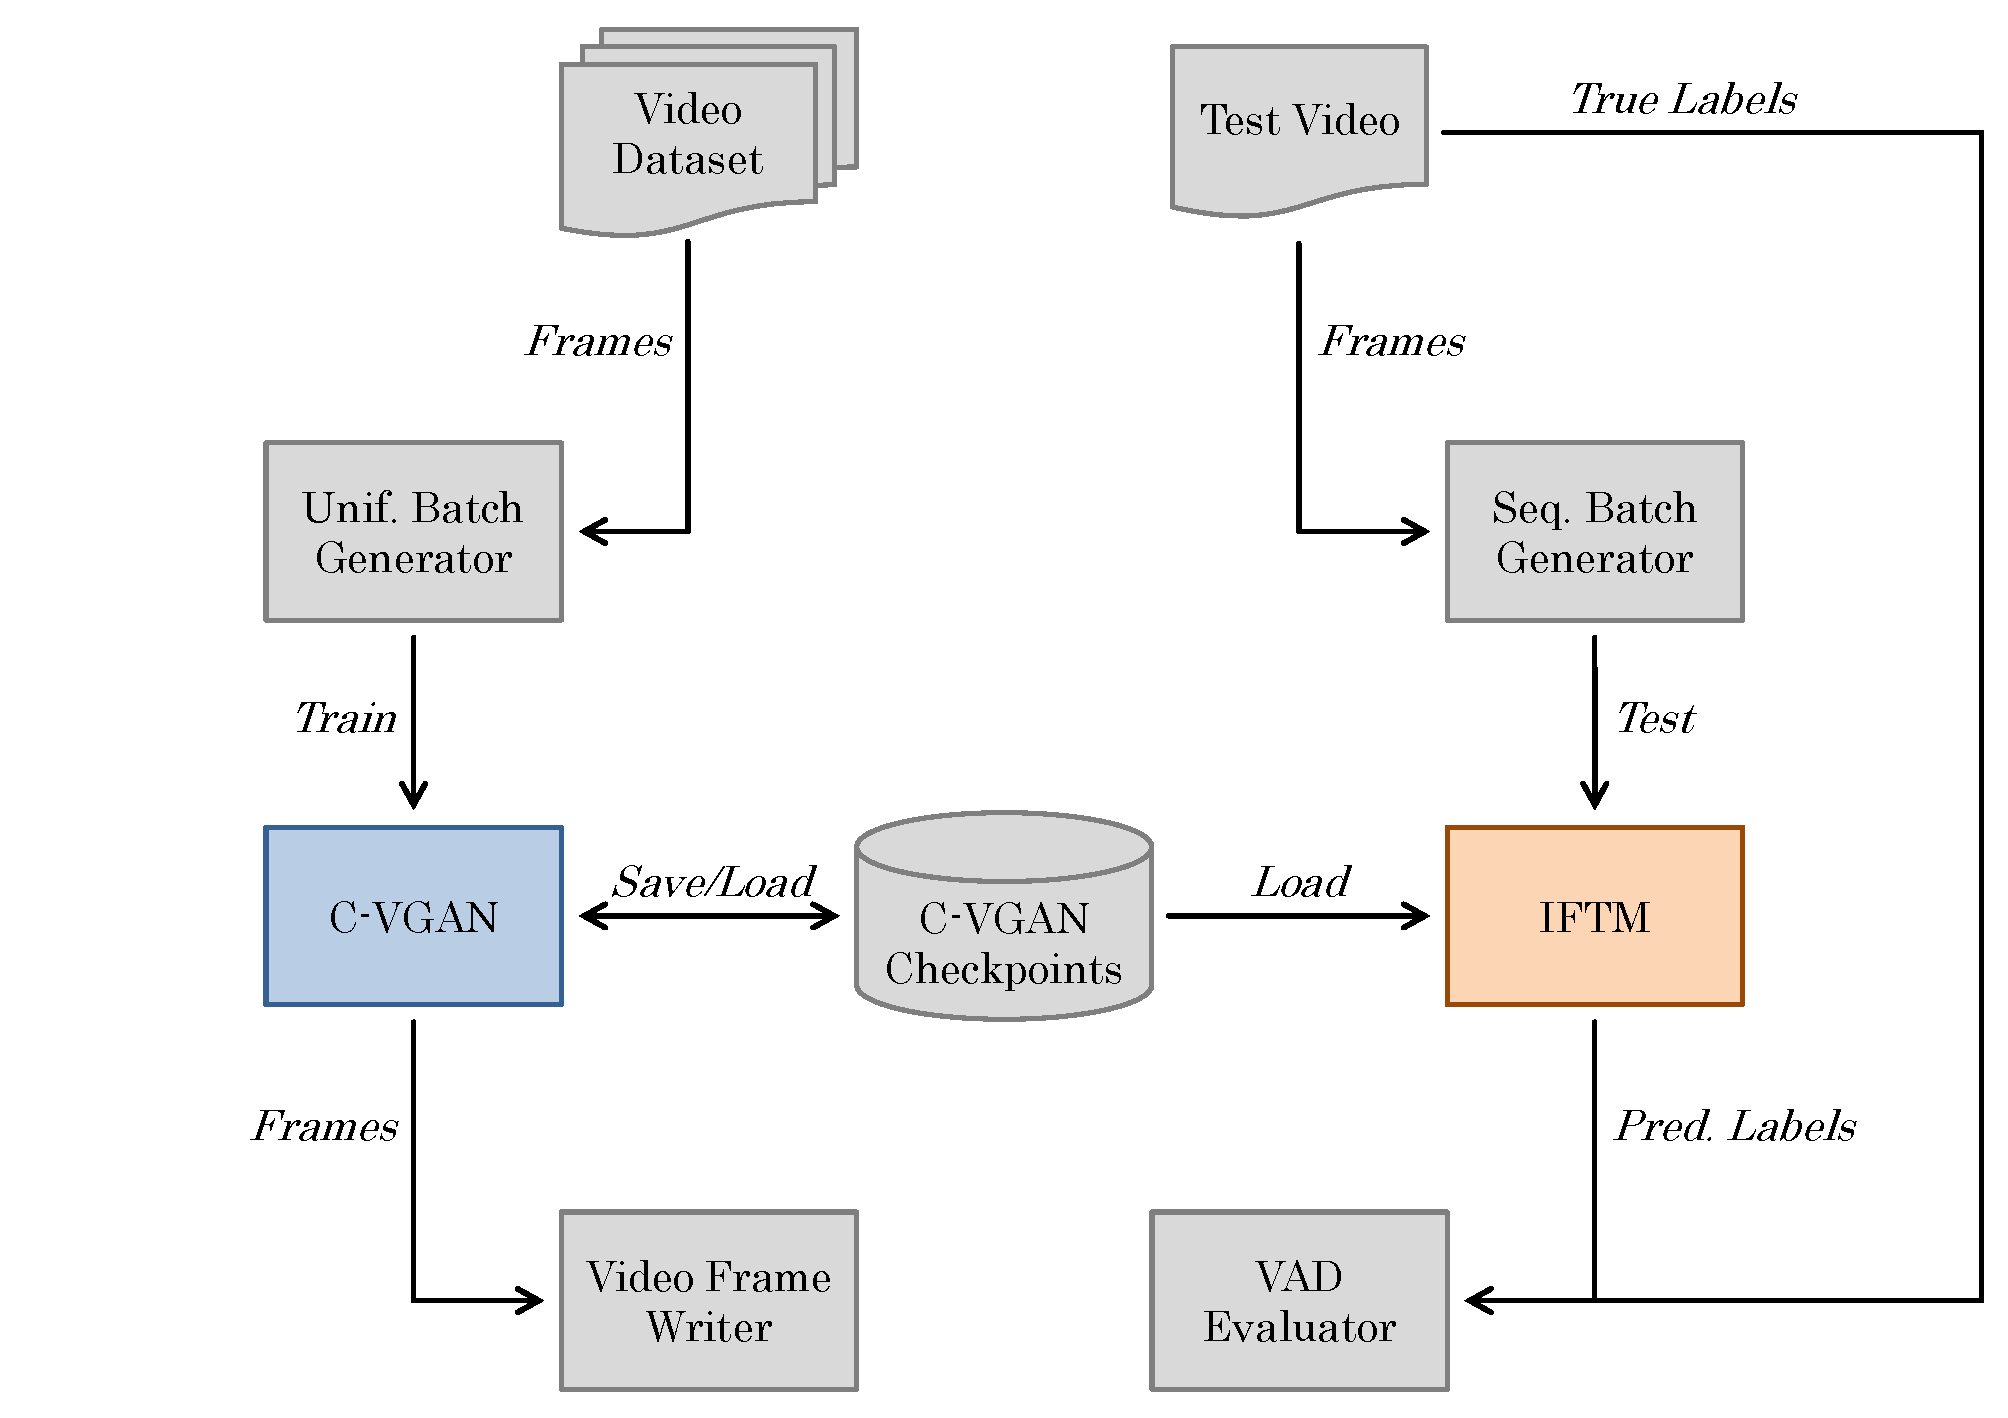
\includegraphics[width=1\textwidth]{graphics/anomalyDetection/ads/system/system.pdf}
  \caption[Components of the video anomaly detection system.]{Components of the video anomaly detection system.}
  \label{fig:ads_overview}
\end{figure}

Putting the different parts of our anomaly detection system (ADS) together, in this section we present an overview of the system depicted in Figure \ref{fig:ads_overview} and go into more detail how we further process the videos that were created and preprocessed as described in the preceding section. Due to the use of a video generation model, the videos have to be first read in a certain way to allow training with the video frames available. We present two batch generators, one to be used during training and a sequential one for evaluation purposes. Afterwards, we explain how the adapted C-VGAN for next-frame prediction is trained and how a trained generator model is loaded and integrated into IFTM at runtime. This includes an overview of the hyperparameters that have to be set. Finally for the last step, we give a brief introduction how the results of both C-VGAN and IFTM are visualized and postprocessed for evaluation.


% Sample and Batch Generation
\subsection{Sample and Batch Generation} \label{subsec:batch_generation}

During training and video generation using the adapted C-VGAN models, the generator and discriminator model only accept 8 frame long videos per sample (a single video clip that is generated or discriminated), and 7 frame long video clips as spatio-temporal input for the next-frame forecasting generator model. So one has to create thousands of smaller video clips from a single video file that can be read in efficient manner. Vondrick et al. during the evaluation of VGAN which requires 32 frames per video clip encountered the same challenge and solved it by concatenating the decoded raw frames of a 32 frame long video clip vertically and saving the resulting file as an image \cite{vondrick2016generating}. Reading these input files requires additional array transformations to transform the 2-dimensional data into a 3-dimensional one, but at the same time it saves additional IO and decoding operations. However, in our use-case, this kind of preprocessing would be redundant: Samples in our case overlap, because the model always has to predict the next frame of the stream and that stream during the detection phase is processed one frame to the next. Meanwhile in the VGAN evaluation by Vondrick et al., the different video clips that were used for training and evaluation were independent from each other. For our data set, the required redundancies to create one image file per video clip would explode the size of the available storage. But even fulfilling the minimum requirement when pre-decoding all videos, i.e. storing every video frame, each decoded as an raw image on a disk is not feasible. It would result in half a gigabyte for $18,000$ frames or one hour of video material, while there are 240 files to be decoded. Furthermore the increase in IO operations would result in a bottleneck, because the frames have to be load from disk individually, every time a sample is generated.

This challenge requires an efficient online decoding of video frames during training of C-VGAN and the anomaly detection phase of IFTM. The video files that are MP4 compressed are loaded into the memory at the start of training and evaluation, but frames and thus samples have to be decoded and created on the fly. Using the OpenCV\footnote{\url{https://opencv.org}} library, one can decode a video frame by frame: Each decoding-call will return a 2-dimensional byte array with three color channels in BGR order. The order of the color channels can be kept this way as it will used for the all training and detection phases and our models do not have a channel order preference. Another challenge exists however in the form of the byte array, which is unuseable by a neural network that works with 32-bit floats. After the necessary type conversion of the entire 2D-array, all pixel color values $x$, which are in the range of $[0, 255]$ are also normalized to a range of $[-1, 1]$ with the following equation:

\begin{equation} \label{eq:norm}
N(x) = \frac{x - 127.5}{127.5}
\end{equation}

\begin{figure}
  \centering
	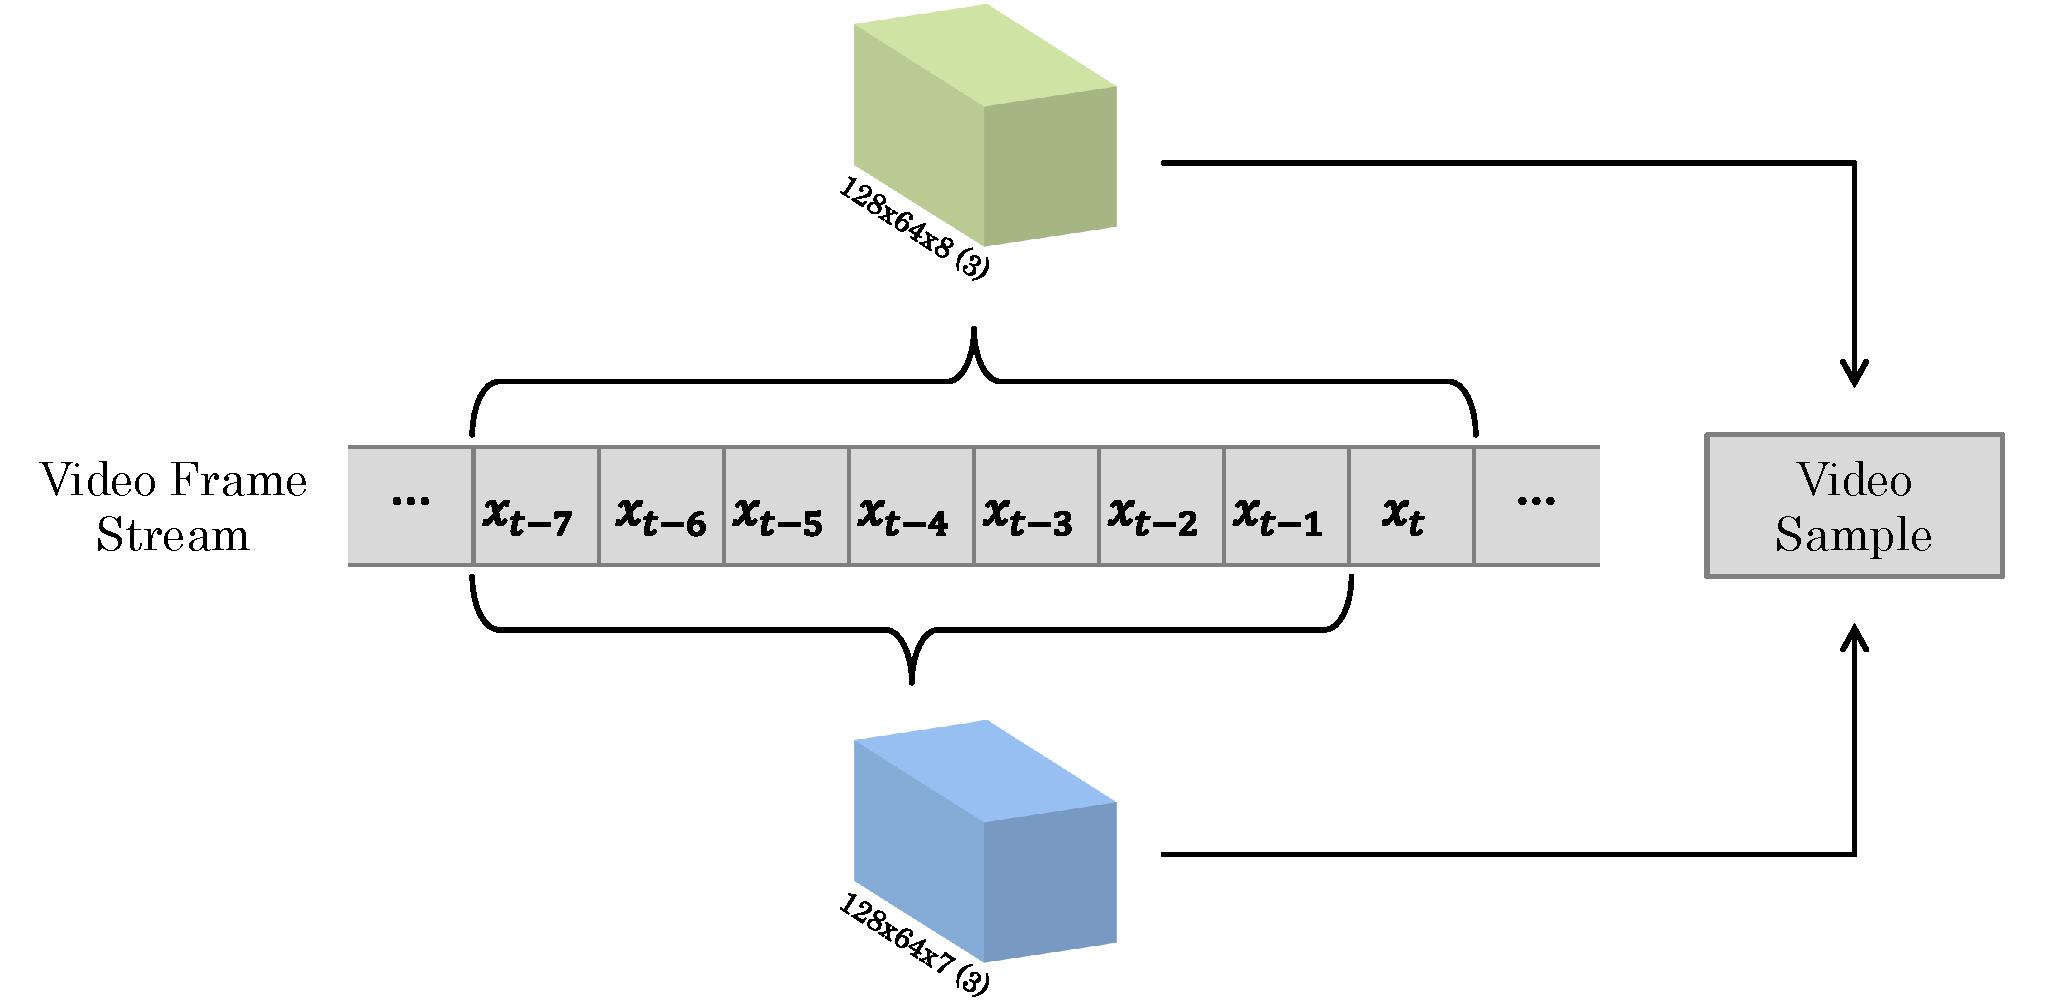
\includegraphics[width=1\textwidth]{graphics/anomalyDetection/ads/sampleGeneration/sampleGeneration.pdf}
  \caption[Creation of a video sample from a frame stream.]{Creation of a video sample from a frame stream, consisting of two video clips arranged as space-time cuboids. The green one serves as input for C-VGAN discriminator, while the blue cuboid will be passed to the generator to perform next-frame prediction.}
  \label{fig:sample_generator}
\end{figure}

This kind of scaling, also used for general DCGANs but also VGAN and C-VGAN, helps with the convergence speed, matching the range of the hyperbolic tangent activation function used in the final layer(s) of the generator \cite{radford2015unsupervised}. Thus, reading a video's frame into arrays, then converting and scaling them, can be used $8$ times to extract the required number of consecutive frames, as shown in Figure \ref{fig:sample_generator}: Stacking the frames as a 3-dimensional cube, this object is duplicated and the last frame is sliced off. The resulting object, a $7$ frame long video clip without its last observation serves as the video input for the next-frame prediction model, while the other one represents the discriminator input. These two together represent a single sample that is passed to the adapted C-VGAN model during training.

Data preprocessing is not done yet, as passing singular samples to the GANs is not the intention during training or testing. GANs are trained by taking a number of samples from the entire training set and passing them to the model as a mini-batch. This is repeated until a percentage of the training data set --- ideally the entire data set,  was passed to the model and this so called epoch is repeated multiple times until a convergence or some other stopping criterion is reached (see Section \ref{sec:gans}). Due to the way the models train and how the inputs are passed and processed by the models, it is important that these mini-batches are ideally sampled independently from the structure of the data. Else a model might learn the structure of the batches during a training step and adapt to it, while being unable to generalize well during testing \cite{bengio2012practical}. Or worse, because during the first batches in an epoch, the model first learns using one type of features witnessed in the batches, before in the second half of the training epoch, it sees the another type. For example, when the video data of a single day is sequentially transformed into batches and then passed to the model, the first batches exclusively contain batches during the day, before only batches with video clips from the night time are witnessed by the models. To improve the quality of the model, some form of randomness for the sample and batch generation is required. First, the overall order of the batches can be shuffled, but for the internal structure of the individual mini-batches, one has to adjust the kind of sampling that is done. Random sampling to create a batch is not only very inefficient but it risks collisions, i.e. sampling the same video clips multiple times during a training epoch, which is also not desired.

As this issue is only relevant during the training phase, because during detection the order of the samples and thus the batches should be treated as a time series, we propose two different batch generators to be used in the two phases respectively. Both of these create samples with the same mentioned structure and the same preprocessing (type conversion and scaling), but the order and structure of the batches and the samples within them differs. The rest of this section will present these and how the two are utilized in our framework shown in Figure \ref{fig:ads_overview}.

\paragraph{Uniform Batch Generator} \label{par:uniform_bgen}
The first of the two batch generators is used during the training phase of the GANs. It attempts to sample the data set in some form of uniform fashion, loading the individual batches of samples in non-sequential order. This has to be done in deterministic and stateless manner, because batch generation will be done concurrently. Else the batch generator is unable to keep up with the training coordinator process of the models. Thus, when loading the videos of the training data set into memory, they are structured as follows: As the number of days is assumed to be fixed but arbitrary, each day is organized as an individual structure. Then, each day is split into six disjunctive subsets of files, therefore four different hours of the day, as shown on the upper half of Figure \ref{fig:uniform_bgen}. This way, when sampling video clips from these disjunctive sets, one gets video clips during both the night and the day when drawing samples from the four respective hours of files uniformly.

To ensure the deterministic and stateless nature, we utilize the id of a batch $b_i$ and map it to a day $d$ and to one of its disjunctive subsets $s$ using Equation \ref{eq:day} and \ref{eq:subset}. Assuming an equal number of to be generated batches per day --- the number not only depends on the sample size (in our case 8 frames), but also on the batch size that is a hyperparameter explained in the next section, one can sample a quarter of a batch from each of the four videos of the disjunctive subset $s$. When doing so, sampling is done in sequential manner starting from an offset $t$ in each of the four videos, as depicted in Equation \ref{eq:offset}. All frames that came before that point were already used by lower batch ids to create samples from. Starting decoding from an offset on an already opened video file can be done using OpenCV. Note that in case of this batch generator, samples in itself are also disjunctive and their frames do not overlap. Because the selection of day, subset, and offset is done based on $b_i$ and the ids are shuffled at the beginning of every epoch, only the order of the batches changes while the internal structure of each $b_i$ remains constant.

\begin{figure}
	\centering
	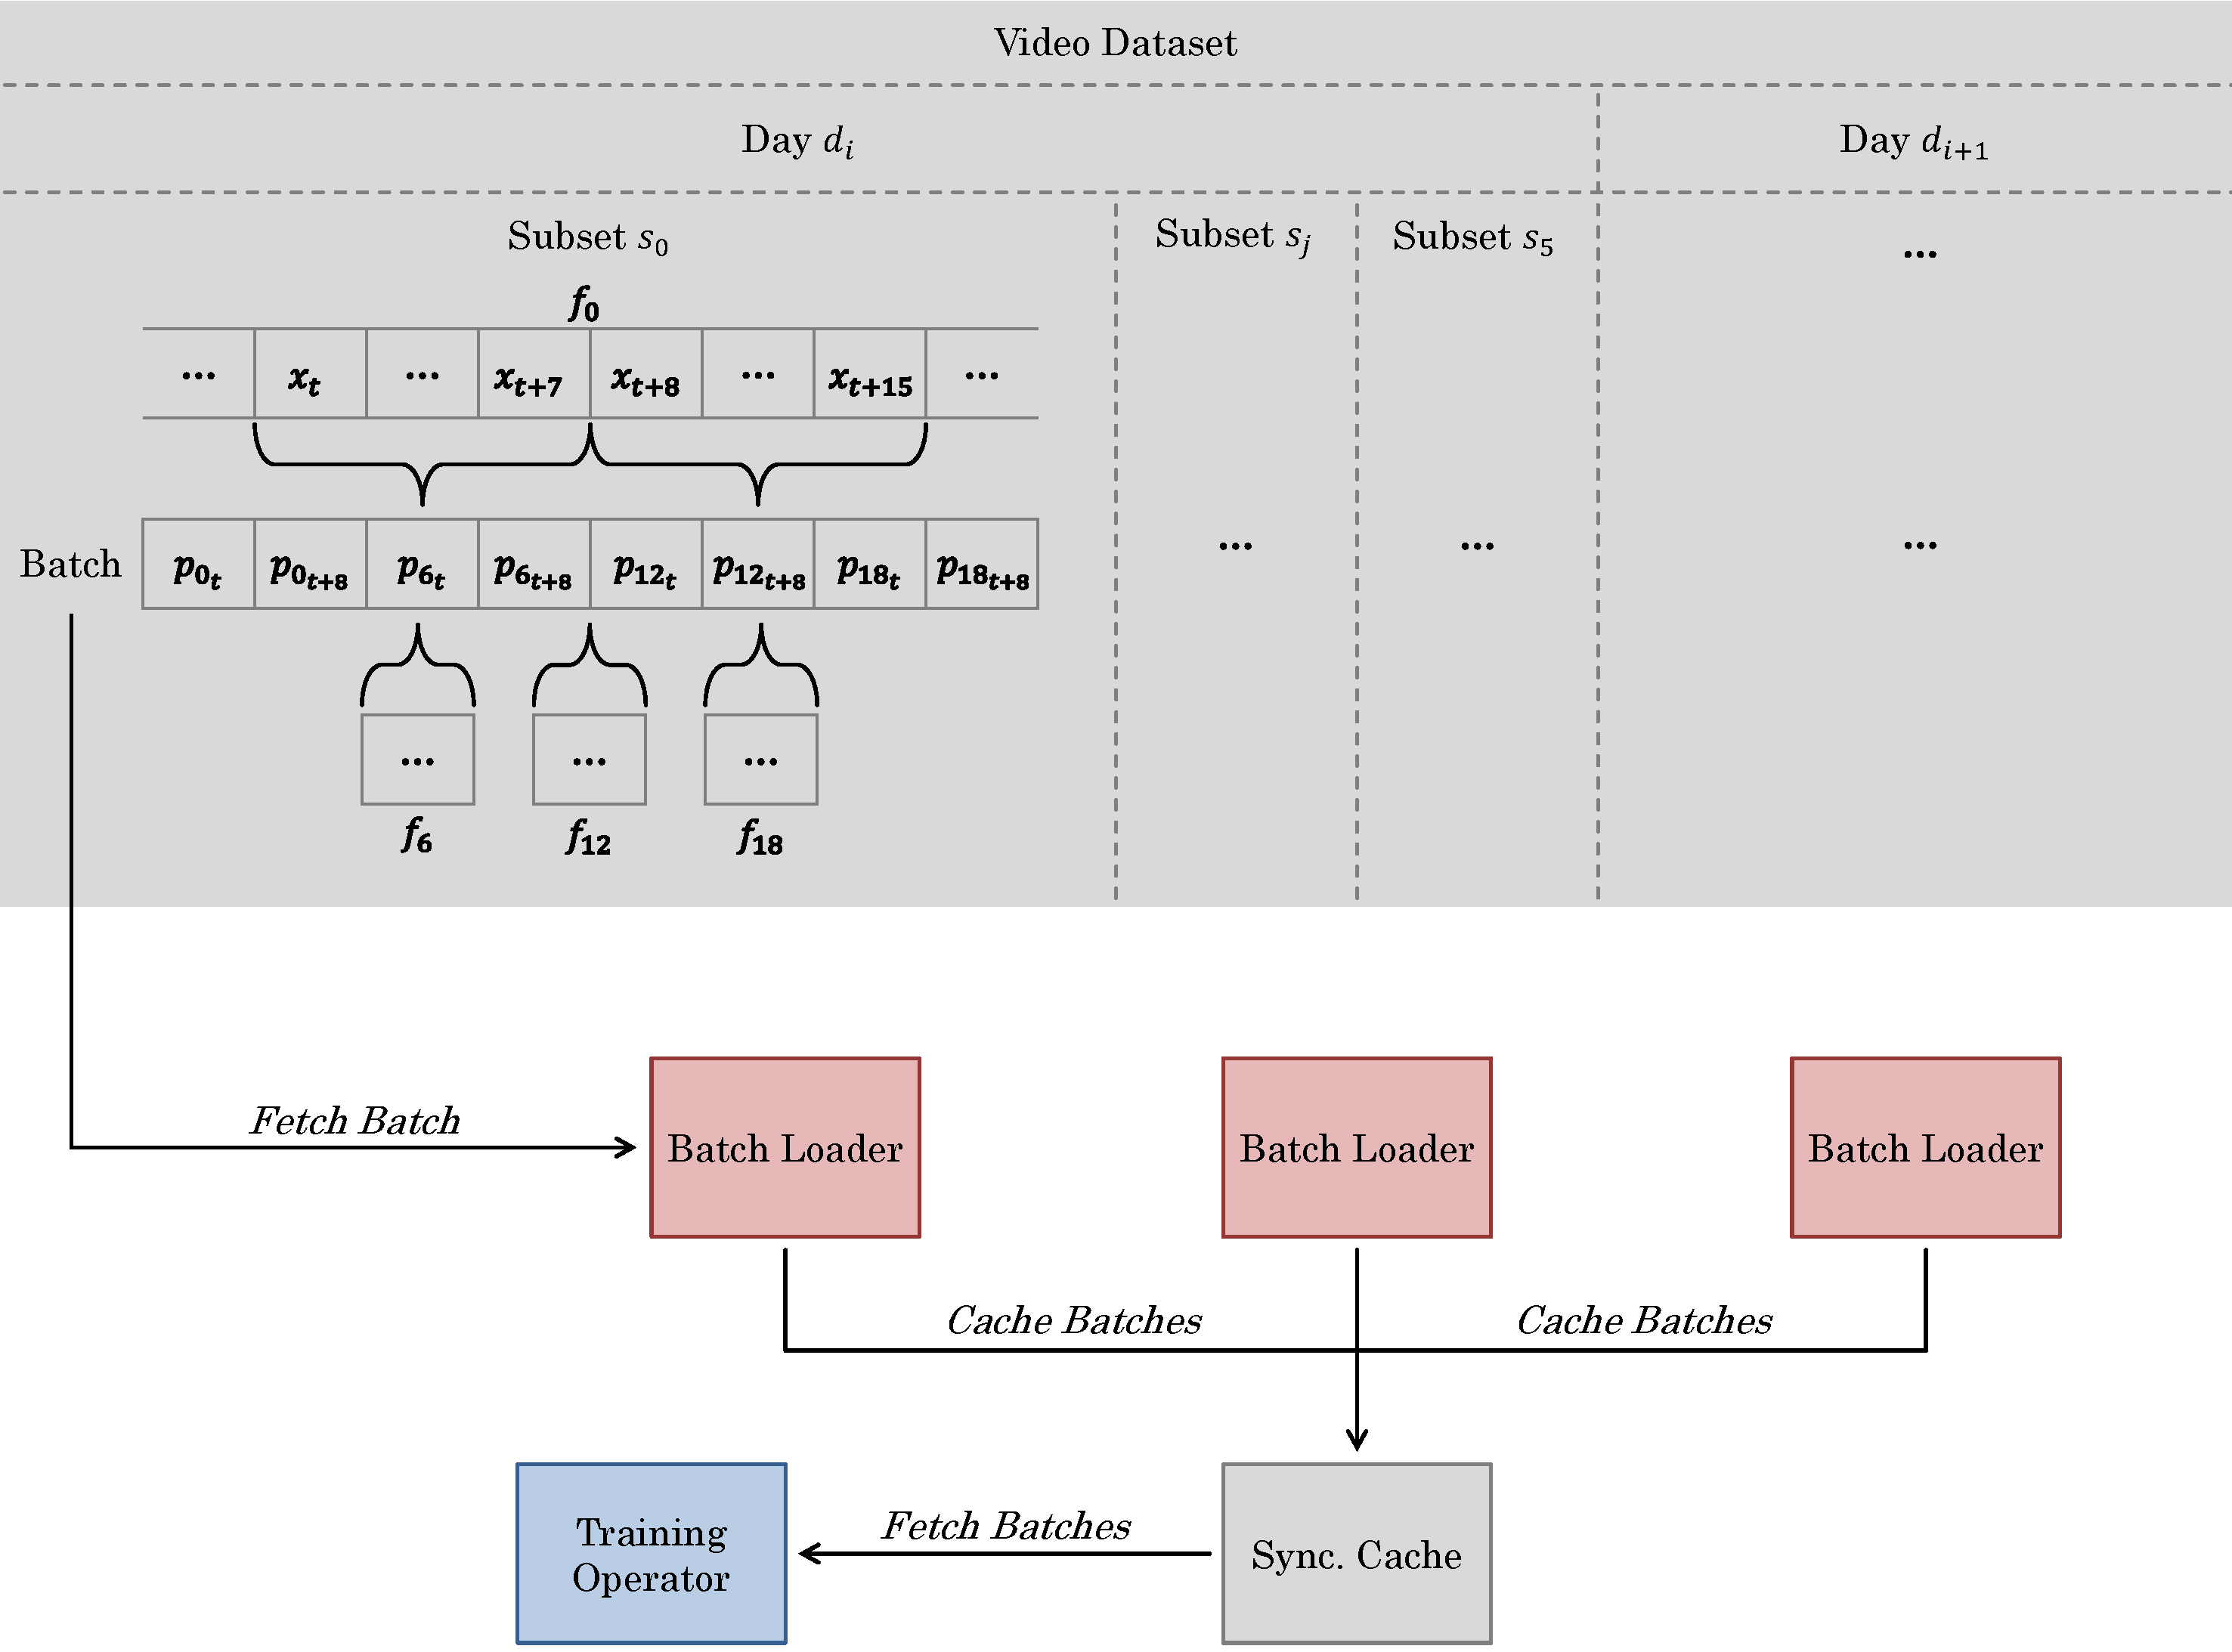
\includegraphics[width=1\textwidth]{graphics/anomalyDetection/ads/batchGeneration/uniform/uniformBatchGenerator.pdf}
  \caption[Creation of a batch sampling from different hours of a day.]{Generation of a batch uniformly sampling from four different files (\textit{f}) of a day, with each file containing one hour of video material. These hours are grouped together in disjunctive subsets (\textit{s}), of which six exist per day (\textit{d}). Batches are fetched from the generator and then cached concurrently by multiple loaders. The operator that handles the training can then fetch ready batches to pass them to the models.}
  \label{fig:uniform_bgen}
\end{figure}

\begin{equation} \label{eq:day}
d = \left \lfloor {\frac{b_i}{batchesPerDay}} \right \rfloor
\end{equation}

\begin{equation} \label{eq:subset}
s = \left \lfloor {\frac{b_i \text{ mod } batchesPerDay}{quarterBatchesPerHour}} \right \rfloor
\end{equation}

\begin{equation} \label{eq:offset}
t = framesPerQuarterBatch \cdot (b_i  \text{ mod } batchesPerDay  \text{ mod } quarterBatchesPerHour)
\end{equation}

As the loading of batches from the batch generator is done concurrently, the access to any video has to be mutual exclusive at any point at runtime. Each of the batch loaders get a shuffled subset of $b_i$ with $i \in [0,N-1]$ with $N$ being the total number of batches that need to be generated. This process is depicted in Figure \ref{fig:uniform_bgen}. Generated batches are passed from the workers to a synchronized cache, from which the operator that coordinates the training of the models draws batches from. This reduces idle times for the training process as the workers in the background provide a constant stream of batches to it. The number of workers and the size of the synchronized cache can be tuned, but they depend on the hardware available and have no influence on the actual quality of the final trained model. During our evaluation, we used $4$ workers to load batches into the synchronized cache that was of size $c = \left \lfloor {\frac{2048}{batchSize}} \right \rfloor$. This cache size proved to be sufficient enough in removing any idle times during training, i.e. the bottleneck was not the fetching of the dataset, but the actual training procedure itself.

\paragraph{Sequential Batch Generator} \label{par:sequential_bgen}

While the generated batches in the training phase can be sampled in any way imaginable, because the adapted C-VGAN model makes predictions for a sample independent from other inputs besides the 7 frames passed to it for a prediction, the detection phase is different: As was explained in Section \ref{sec:vad}, IFTM, as modified to our use case, makes forecasting, computation of the prediction error, and the mapping to the binary label (anomaly or not) online, treating the video data as a stream. Although this is doable in real time, it is not desired during evaluation: Because the C-VGAN models are deployed on a GPU as explained in the following section, one can make use of all the video memory and processing units available and parallelize this part of the evaluation system as well for major speedups \cite{owens2008gpu, abadi2016tensorflow}. But running several next-frame predictions for a multitude of samples at the same step in parallel, implies that some form of batch generation is required again. 

To keep the samples in order of their occurrence in the stream, samples are aggregated into batches following Figure \ref{fig:sequential_bgen}: This time, files are structured as a list from which samples are generated from, one file after another. For each file, samples are created by sliding a window with size $8$ with step size $1$ over the frames and this is done until the required number of samples for a batch have been created. Same as the other batch generator this process can be done deterministically and statelessly, by mapping batch id $b_i$ again to a file ($f$), illustrated in Equation \ref{eq:day2}, before reading samples starting from position $t$ of the selected video file. This again assumes videos of equal length and thus number of frames.

\begin{figure}
	\centering
	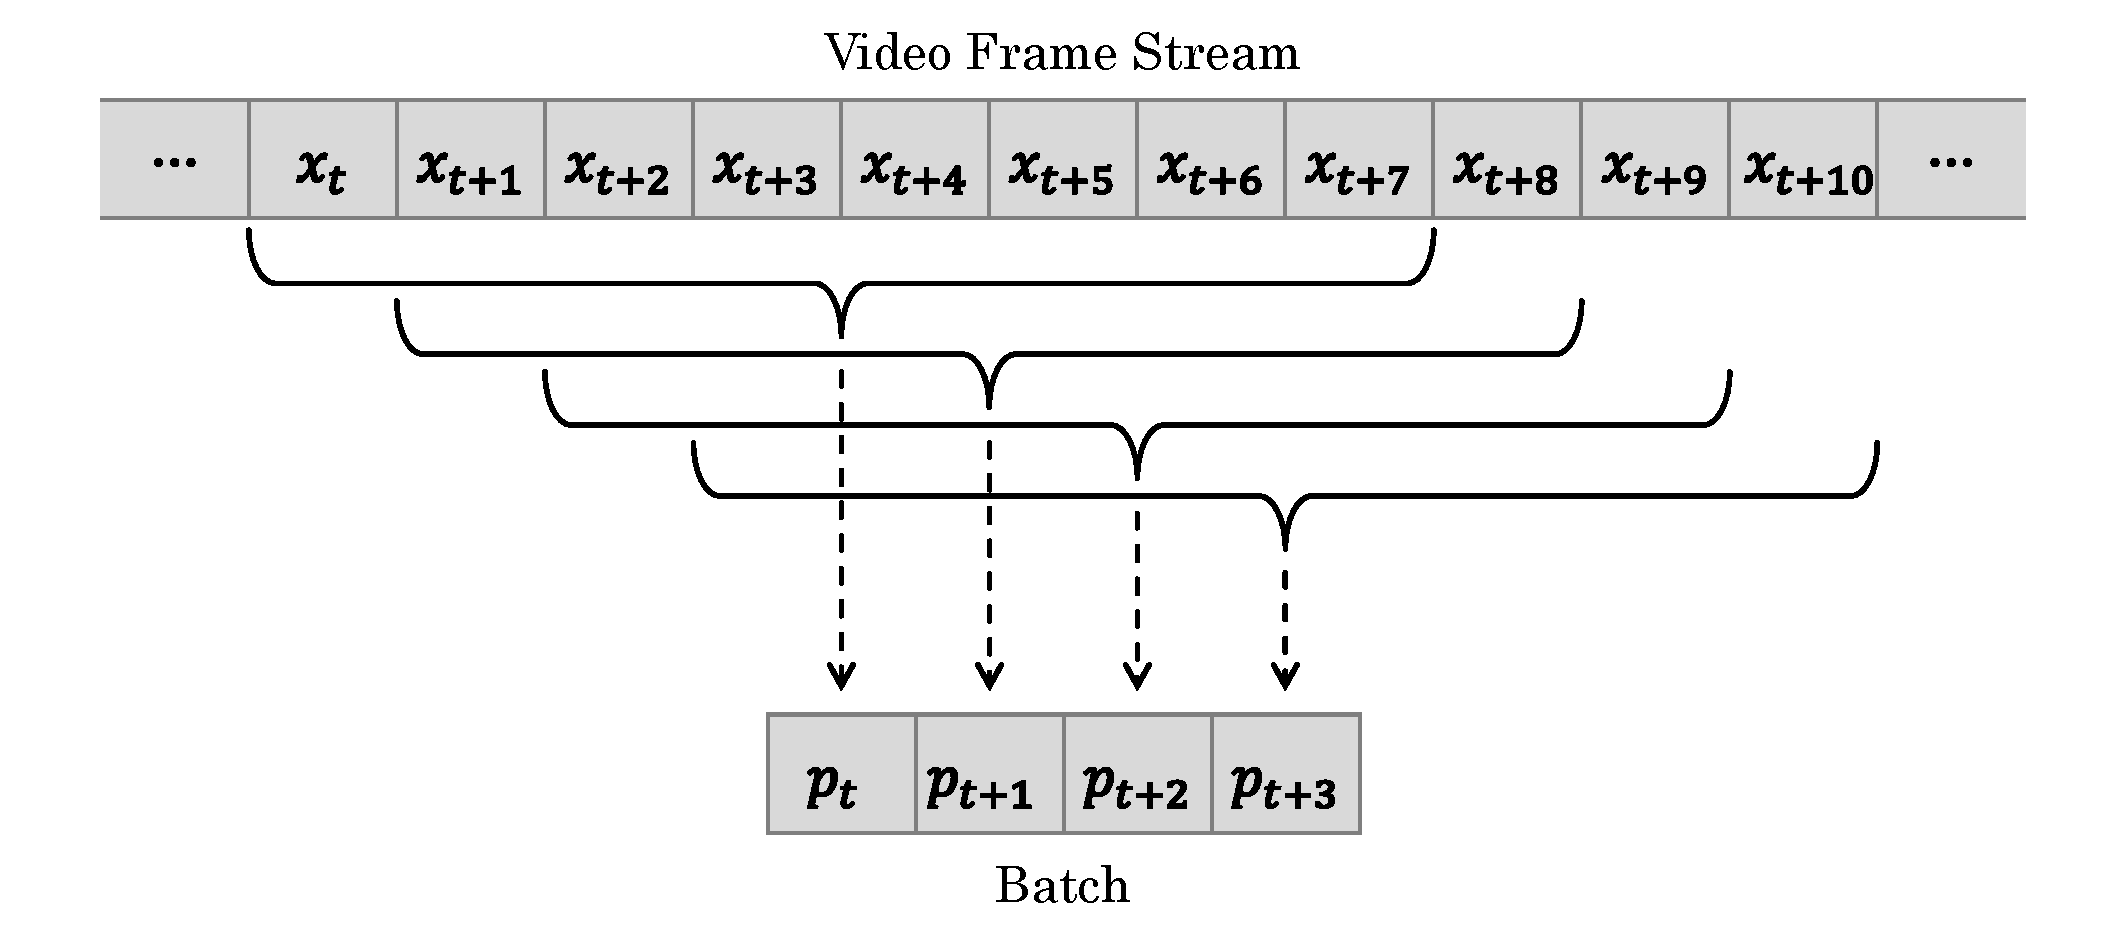
\includegraphics[width=1\textwidth]{graphics/anomalyDetection/ads/batchGeneration/sequential/sequentialBatchGenerator.pdf}
  \caption[Creation of a batch that consists of consecutive samples.]{Creation of a batch that consists of four consecutive and overlapping samples, using a sliding window to aggregate frames into samples (\textit{p}), and samples into batches.}
  \label{fig:sequential_bgen}
\end{figure}

\begin{equation} \label{eq:day2}
f = \left \lfloor {\frac{b_i}{batchesPerFile}} \right \rfloor
\end{equation}

\begin{equation} \label{eq:offset2}
t = framesPerBatch \cdot (b_i  \text{ mod } batchesPerFile)
\end{equation}

Although one could now use this sequential batch generator with multiple workers to fetch data faster, it is not advised due to the inherent order of a stream: Unlike in the other generator, batches can not be read out of order, nor can they be placed in the synchronized cache in an arbitrary one, because the samples in every batch have to be matched to their true labels for evaluation. This requires some overhead to synchronize the write order for multiple batch loaders. Meanwhile in our data set presented in Section \ref{sec:dataset}, there is only one video file that has to be read in that manner, which makes such a speedup not only unnecessary, but also impossible. As already mentioned above, access to a video is mutual exclusive, so different batch loaders would only alternate their access to that single video file between each other. Compared to the $240$ video files of the training set, reading the much smaller evaluation set can be done in this evaluation framework with a single worker, creating batches in order. It is to note however that the batch size has no influence on the results during prediction and thus can be as great as the video memory permits, providing some additional speedup. 


% C-VGAN Training, Model Creation
\subsection{C-VGAN Adaption} \label{subsec:framework_cvgan}

\begin{table}
	\centering
	\begin{tabular}{ | l | p{9cm} | r |}
	\toprule
	\textbf{Hyperparameter} & \textbf{Description} & \textbf{Default Value} \\
	\midrule
  $\lambda$ & Weight of the reconstruction loss term for the first 7 frames of the generator output. Limits the degrees of freedom, i.e. how much past frames determine the forecasting. & $10$ \\ \hline
  $cf$ & Number of convolutional filters (channels) in the first layer of the discriminator. The value is doubled for each consecutive step of the CNN stack. Greater values empower the model, while smaller ones impair it.  & $32$ \\ \hline
  $dr$ & Dropout rate at which input units after every convolutional layer in the discriminator get randomly set to 0 during training. Regularization parameter. & $0.0$ \\ \hline
  $bs$ & Batch size; number of samples that are passed to the models at each training step. & $64$ \\ \hline
  $lr$ & Learning rate; step size of optimizers during training. & $0.002$ \\
	\bottomrule
	\end{tabular}
	\caption[Hyperparameters of the modified C-VGAN next-frame prediction model.]{Summary of the non-fixed hyperparameters of the modified C-VGAN next-frame prediction model.}
	\label{tab:cvgan_params}
\end{table}

For building our proposed adapted architecture for next-frame prediction, we take the two models presented in Section \ref{subsec:vgan_mod_2} and define them using TensorFlow. TensorFlow, as the name suggests, uses dataflow graphs to represent computations and the operations that mutate the states in it \cite{abadi2016tensorflow}. Because our model consists of two components --- a generator and a discriminator, that have to be trained in adversarial fashion, we define the two models using the functional API by Keras that serves as an abstraction layer ontop of TensorFlow \cite{chollet2015keras}. For the training procedure, we define a custom training loop. At each step during training, the current batch is passed to the discriminator and the generator, with the latter one using the first 7 frames of the sample as input. Losses are computed using the adapted value function of C-VGAN for next-frame prediction. For optimization of the models the Adam optimizer \cite{kingma2014adam} was chosen; one for the discriminator and another for the generator model. In VGAN and C-VGAN, Vondrick et al. use Adam with a learning rate of $0.002$ and a momentum term of $\beta = 0.5$, while using a batch size of $64$. For training models the batch size serves as a hyperparameter, because the value function is computed over the entire batch, i.e. the losses for each sample in the batch are computed and then summed up. This however can bring additional hurdles, if the batch size is large, but the data set is diverse \cite{radiuk2017impact}: Meaningful observations in the batch might get discarded and ignored, because the total loss for a batch is driven by the majority. And with the model being tuned through the minimization of the loss for each batch, rare but normal observations will not find their representation within the model. But at the same time a large batch size also helps with suppressing anomalous observations that might be encountered in the training data set. Although Adam is an adapted optimizer, its learning rate might need adjustment when tuning the batch size \cite{krizhevsky2014one}. To keep the variance of the gradient expectation constant, the learning rate is multiplied by the square root of $k$, with $k$ being the factor by which the batch size was increased. The momentum was chosen to stay fixed and mirrors the original configuration of DCGAN and VGAN.

The other hyperparameters for both generator and discriminator, that were already explained in detail in Section \ref{subsec:vgan_mod_2}, also have to be set. Their default values are also included in Table \ref{tab:cvgan_params}. When setting these hyperparameters and training the configured model, training has to be done for several epochs over the training set. Because training takes up to $2$ days of computations (see the next chapter), intermediate results of the models are stored to disk after every $N$ epochs, with the hyperparameter configuration attached. This not only serves as fault tolerance, but also a means to evaluate different configurations in quick succession by simply loading and evaluating one after the other. In addition, one can load and evaluate a model from different points in training, to see whether the quality of the model has degraded over the epochs; see Section \ref{par:failure_modes} for details regarding collapse in training and early stopping.

For the evaluation in the next chapter in Section \ref{sec:cvgan_eval}, the losses per batch are averaged and logged for each epoch during training. Moreover, after each epoch one can also validate the quality of the current models with a separate validation data set and the average batch loss is then also logged.


% IFTM Training, Predicting
\subsection{IFTM Adaption} \label{subsec:framework_iftm}

To load offline trained models into the adapted version of IFTM from Section \ref{sec:vad} to perform VAD, one has to select one of the stored generator models from the preceding section. Loading it via the TensorFlow checkpoint API\footnote{\url{www.tensorflow.org/guide/checkpoint}}, that forecasting model is then defined as the IF of the IFTM anomaly detection model. Afterwards, as explained in the adaptation of IFTM, all training samples used during the training of the generator model have to be passed to the model again to compute the prediction error for their respective 8th frame. Aggregating the distribution of the errors into its mean and standard deviation, one can now compute the (static) threshold value for the IFTM. There are no additional hyperparameters for this version of IFTM beside the ones for the underlying next-frame forecasting model, which do not change after loading the checkpoint.

As this procedure concludes the offline training phase, the detection phase begins: Using the sequential batch generator, batches of samples are passed to the IF to perform next-frame prediction. Afterwards the prediction error and the mapping to the binary label, 0=normal and 1=anomalous, is done for each sample in the batch. For evaluation purposes, the error value and the binary prediction for each sample are logged as a tuple. Based on the former metric, we will also analyze in the next chapter how IFTM using video generation forecasting models performs on our evaluation data set.


% Evaluation and Visualization
\subsection{Postprocessing} \label{subsec:postprocessing}

When postprocessing the generated video samples of C-VGAN, forecast frames for the evaluation data set are written to disk as PNG images for visual evaluation, i.e. how realistic these predictions actually are. Doing so, the data type is also reversed to 8-bit format and a scaling of each pixel color value of $[0,255]$. In addition, during training, a fixed set of input samples are passed to the forecasting model to run a prediction on after every epoch. These predictions are also written to disk as animated GIFs to monitor the quality of the generated videos. In Section \ref{subsec:cvgan_eval_method} of the next chapter, an in-depth overview of the evaluation methods for the next-frame prediction model is provided.

For the evaluation of the VAD system using IFTM, its binary predictions for each sample are compared to the ground truth, as the true label of each frame in the evaluation data set is available in a separate CSV file. The results of thereof are aggregated into a confusion matrix, which can then be utilized to compute several metrics to measure the quality of the model. In the following chapter in Section \ref{subsec:vad_eval_method} we will show our chosen evaluation metrics for IFTM, and how they are inferred from the matrix, before we present and discuss our results for different configurations of the underlying models.  % 30-40

\chapter{Results} \label{chap:results} % 20-30 pages

This chapter presents and discusses the evaluation of the proposed anomaly detection approach for video. As described in the previous chapter, evaluation of the anomaly detection system (ADS) is done by first training the video generation model for next-frame prediction, before that model is loaded into IFTM (see Section \ref{sec:framework}). The resulting ADS is then run on a labeled evaluation video data set. Evaluation of the two components is decoupled at first: In Section \ref{sec:cvgan_eval}, the evaluation method and the results for the video prediction model are presented. Then in Section \ref{sec:vad_eval}, the quality of the IFTM ADS using the already evaluated prediction models is assessed. Finally in Section \ref{sec:discussion}, both results are discussed and linked to each other.

Evaluation was performed on a workstation running Windows 10 with 32 GB RAM, a 4.2 GHz Intel i7 quad-core processor, and a Nvidia GeForce 3090 graphics card with 24 GB VRAM. A full evaluation run of a single hyperparameter configuration usually took 24--48 hours depending on the configuration and the load of the system. An implementation of the analysis framework is available online\footnote{\url{https://github.com/fshofmann/video-anomaly-detection}}.



% C-VGAN Evaluation
\section{C-GAN for Video Forecasting} \label{sec:cvgan_eval}

For the evaluation of video generation models, the focus in this work lies solely on our modified version of C-VGAN presented in Section \ref{subsec:vgan_mod_2} and not on any of the preceding versions. As explained in Section \ref{subsec:framework_cvgan}, our framework saves any models during and after training to disk, to allow them to be used for anomaly detection evaluation. To find optimal prediction models for this task, these models need to be evaluated on their own without direct connection to the task of video anomaly detection (VAD). However it is unfeasible to evaluate many hyperparameter configurations due to the high number of trainable parameters in the two models, that need to be optimized until a convergence of losses of the two adversarial models is achieved (see Section \ref{sec:gans}). Therefore as explained in the presentation of the framework, the number of non-fixed hyperparameters is heavily limited and their initial values are based on configurations of DCGAN \cite{radford2015unsupervised}, VGAN, and C-VGAN \cite{vondrick2016generating}. Training of each configuration is fixed to 50 epochs, since most models maintained their loss-equilibrium till that number of training iterations.

The performance of all configurations is evaluated based on quantitative evaluation metrics but also on qualitative ones, i.e. visual, assessment. The reasoning behind that will be explained in the following section, while further insight into these metrics will be provided as well. Afterwards the results for our models using different hyperparameter configurations are presented. This includes additional information on the tuning of thereof.


% C-VGAN Evaluation Methods
\subsection{Evaluation Method} \label{subsec:cvgan_eval_method} % 3 Pages

\paragraph{Hold-Out Validation}
First, to evaluate a model on its ability to predict the next frame from a fixed set of past frames, the quality of the model cannot be assessed using observations with which the model was trained. Worst case, models are able to accurately reflect the training observations and thus make perfect predictions for them, while being unable to work with unknown inputs at runtime. However at the same time, the evaluation data set presented in Section \ref{sec:dataset}, is not helpful to evaluate the quality of a next-frame prediction model. At least from a generalization perspective: As this data set tries to disrupt the prediction model by giving it both normal and anomalous videos, the model must be unable to model these anomalous properties found in that data set and make predictions that differ to the actual videos. Therefore a good generalization performance on that data set would cause an equally bad anomaly detection performance, as IFTM would be unable to differentiate between the predictions errors of normal and anomalous observations.  

\begin{figure}
	\centering
	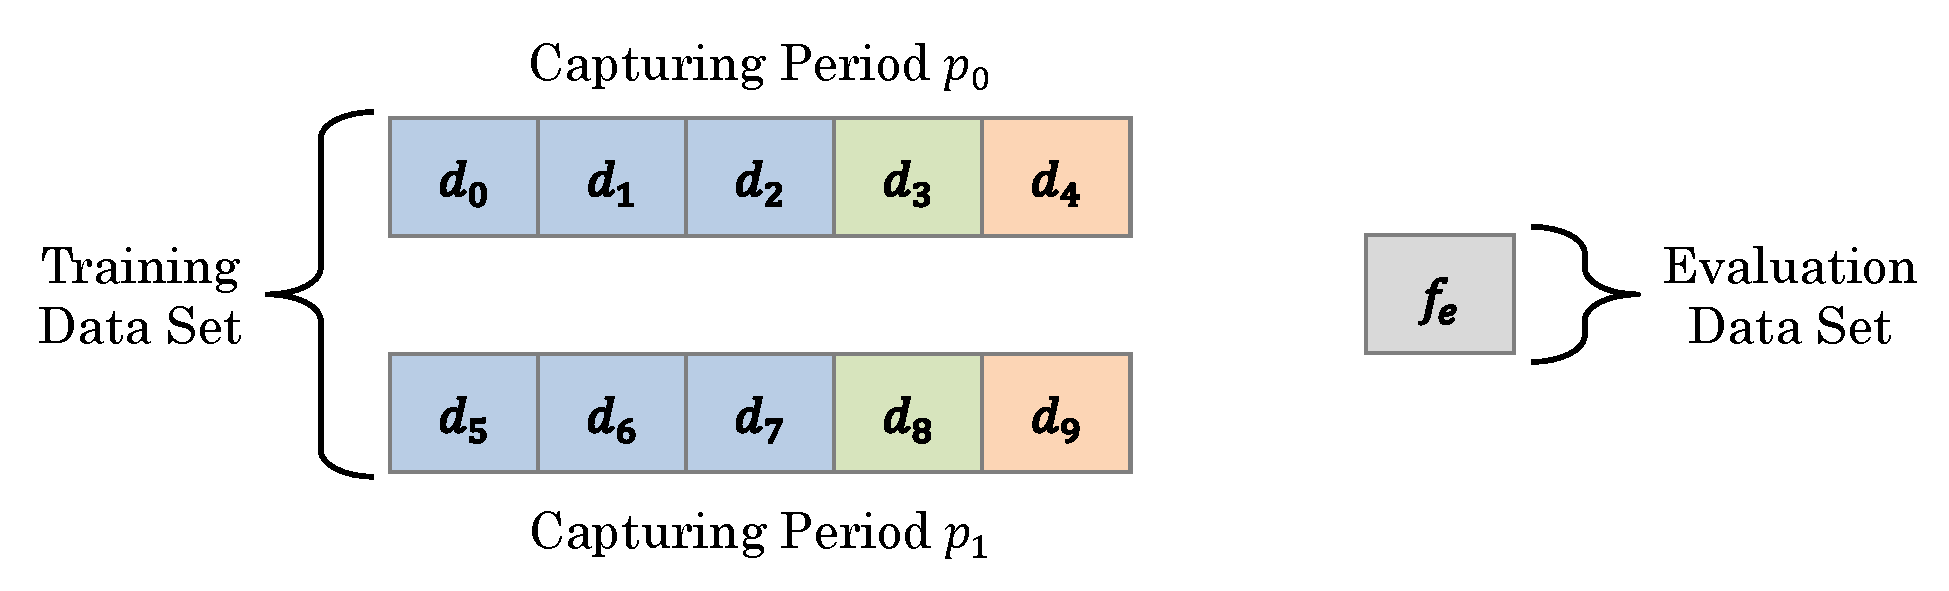
\includegraphics[width=0.9\textwidth]{graphics/eval/evalSplit/evalSplit.pdf}
  \caption[Splitting of the data set for evaluation.]{Splitting of the data set into training (blue), validation (green), and test set (orange). The evaluation data set (gray) is used at a later stage and relevant for the prediction model's qualitative evaluation.}
  \label{fig:dataset_split}
\end{figure}

Thus the training data set consisting of $10$ days is further split into three parts, as illustrated in Figure \ref{fig:dataset_split}. Six days, three from each capturing period (see Section \ref{sec:dataset}), will be given to the model during training. Then, the model's quality is validated after the completion of every training epoch using two other days of video material. Lastly, the remaining two days are chosen as the test set to measure the quality of the final model independently from the tuning of the hyperparameters. This kind of hold-out validation with fixed subsets is to be preferred over exhaustive cross-validation methods in which all combinations of subsets are used to train, validate, and test the model iteratively, before the respective errors across runs are averaged \cite{stone1974cross}. The long time to fully train a single model configuration --- up to $48$ hours, makes the latter methods unfeasible for this work, as they would greatly reduce the number of different hyperparameter configurations one can explore and evaluate. 

\paragraph{Model Losses}
Training, validating, and testing the model require the measuring of the models' value function, that is optimized during training. As GANs consist of two models that play a min-max game to optimize said function, as explained in Section \ref{sec:gans}, one can take said function and disassemble it into the loss terms that are minimized by each of the two models. Applying this to the adapted value function of C-VGAN for next-frame prediction from Section \ref{par:vgan_mod_2_vfn}, this results in the following loss functions for the generator $G$ and discriminator $D$, respectively:

\begin{equation} \label{eq:loss_g}
\mathcal{L}_G = \mathbb{E}_{x_{0;6} \sim p_{x_{0;6}}(x_{0;6})}[\log(1 - D(G(x_{0;6})))] + \mathbb{E}_{x_{0;6} \sim p_{x_{0;6}}(x_{0;6})}[\lambda \cdot \|(x_{0;6} - G^{0;6}(x_{0;6}))\|_1]
\end{equation}

\begin{equation} \label{eq:loss_d}
\mathcal{L}_D = - \mathbb{E}_{x \sim p_x(x)}[\log D(x)] - \mathbb{E}_{x_{0;6} \sim p_{x_{0;6}}(x_{0;6})}[\log(1 - D(G(x_{0;6})))]
\end{equation}

During training, these losses are computed batch wise, i.e. for each training step in an epoch, and the average of thereof is computed at the end of every epoch for evaluation purposes: Disregarding the reconstruction loss (second loss term of $\mathcal{L}_G$), training of the two models is a zero-sum game in which both models' losses should converge to non-zero values over the epochs, as they improve in parallel. Failure to converge is a sufficient indicator for a failure mode in training and a high certainty that the models are of poor quality; see Section \ref{par:failure_modes} and the paragraph about the common failure models in GAN training. In addition, after the completion of every epoch, the models are validated using the validation split of the data set and the models' validation losses are computed and recorded as well. The same is done with the test data set after the entire training procedure is completed. It is to note, that validation and test losses are only of use if failure to generalize is one-sided and does not affect both models, as the loss functions influence each other. But even if the latter occurs, differences in the losses' behavior during training can be of interest. For example it would be ideal if both training and validation losses converged in similar manner. Any fluctuations of the validation losses while training losses were stable would be an indicator for overfitting models that are not able to generalize well. Finally, the generator loss also serves as a strong indicator whether the generator is even able to reconstruct past frames, as, depending on the choice for $\lambda$, the reconstruction term is dominating the generator's loss function.

\paragraph{Qualitative Evaluation} \label{par:cvgan_eval_method_qual}
While failure modes in the training of GANs are most of the time an indicator that something has gone wrong and the models have to be discarded, a successful convergence of the losses does not imply the GANs have successfully completed training: Failure to model certain motion dynamics, hallucinating or the omission of objects, or simply the generation unrealistic looking videos can still occur. This happens sometimes when either the capacity of the generator is not sufficient to learn all video properties or if an optimal discriminator does not provide enough information for the generator to improve on its synethetic outputs; the latter problem that can be traced back to vanishing gradients was also found in the generator models of GANs \cite{arjovsky2017towards}. But even if all of these failures do not occur, it is challenging to use the converging losses as an indicator when to stop training: The retention of the equilibrium in losses can either mean that the models are still continuously and in parallel improving, or that the training procedure has been completed and more epochs will not lead to any changes in the quality of the generator's outputs. To actually check up on the models' progress and its outputs' quality, one has to inspect the generator's output and evaluate it on its own.

But the task of evaluating the quality of generative models is a hard one, as is the automation of thereof, and there is no standard evaluation protocol: Often one has to rely on human workers that have to manually decide whether the synthetic outputs or the real observations are more realistic to them. The percentage of these so called video generation preferences over the real observations is then used to compare a approach to other existing ones. VGAN and its offshoots are evaluated in that manner \cite{vondrick2016generating, tulyakov2018mocogan, spampinato2018vos, spampinato2019adversarial}, using the platform Amazon Mechanical Turk\footnote{\url{https://www.mturk.com/}} with the same constraints on the selection process for their workers and using comparable data sets. For future frame prediction approaches including C-VGAN by Vondrick et al., qualitative evaluation is however done differently \cite{vondrick2016generating, vondrick2017generating, jang2018video, talafha2020attentional}: While the realness of a synthetic output --- a video prediction, is still of interest, the transition quality from past to future frames and the predicted future's plausibility has to be qualitatively evaluated as well. But in the end there is no evaluation standard for them either.

Thus as the first step of the qualitative evaluation, after the validation of the models upon completion of an epoch, a fixed set of $16$ input videos sampled from the test split is also passed to the next-frame generator model to make predictions on. The synthetic videos for each epoch are then manually inspected by a human whether their quality improves or degrades between different epoch numbers. The definition of quality in that step is broad and includes: The general sharpness of the scene and any of its objects, the reduction of noise and grain in the video, the reconstruction of object patterns --- especially people, and the minimization of hallucinations by the next-frame prediction model. These are necessary conditions for a good prediction model, and serve as a first filter to determine whether training of a model is completed or whether it is actively degrading (see Section \ref{sec:gans}).

\begin{figure}
	\centering
	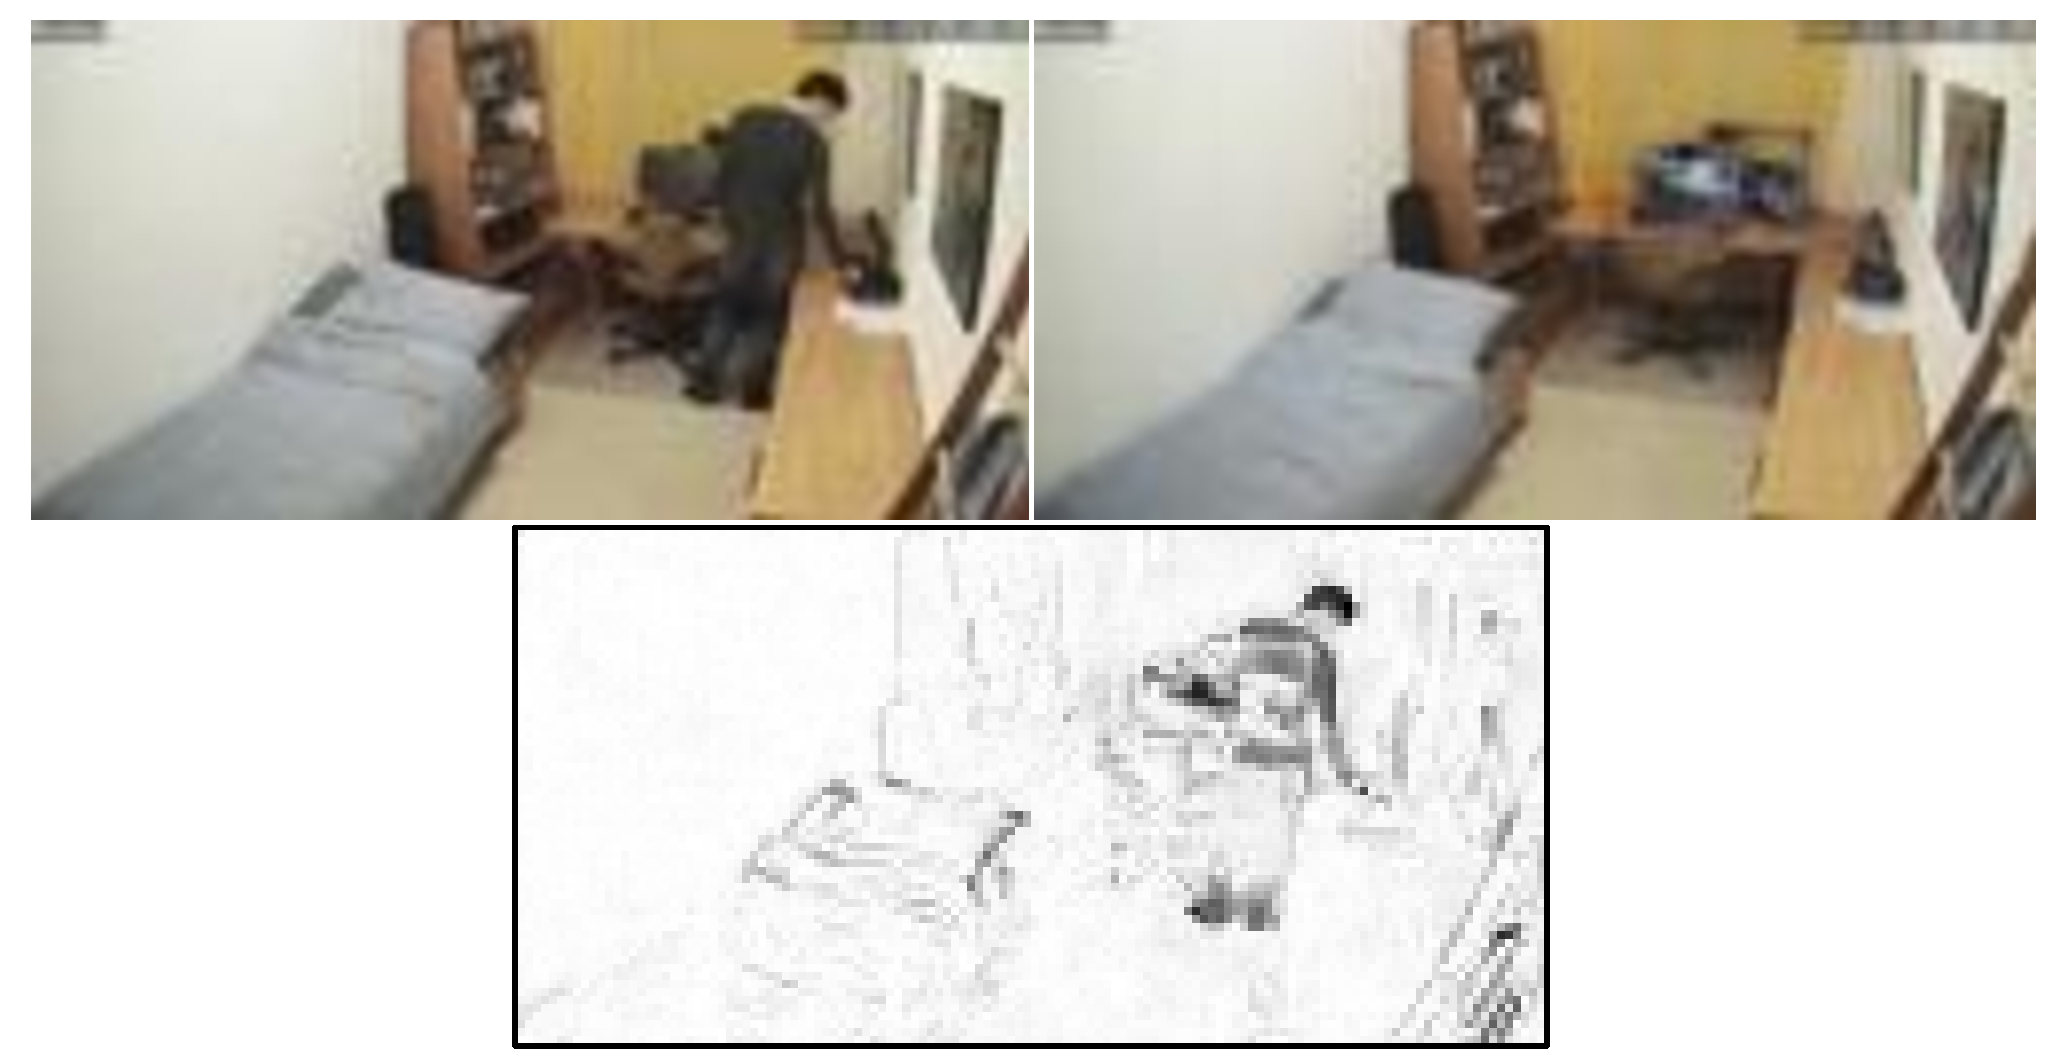
\includegraphics[width=0.8\textwidth]{graphics/eval/heatmap/heatmap.pdf}
  \caption[Exemplary heat map of the mean absolute error per pixel of a predicted frame.]{Exemplary heat map of the mean absolute error per pixel of a predicted frame. The heat map can be computed by comparing the actual frame (upper left) to the predicted future (upper right).}
  \label{fig:prediction_comparison}
\end{figure}

While the mentioned criteria can also be used to discriminate different models quickly, a qualitative evaluation of the predicted future is still missing. Evaluating a prediction is difficult as the future is uncertain and there are several if not infinite plausible outcomes that can be inferred from the past. Even for our next-frame prediction model, the 8th out of seven frames can take multiple shapes and it would be naive to simply compare the prediction to the actual observation and evaluate the model's quality based on that. On the other hand, the next-frame prediction models are integrated into IFTM and their predictions are compared to the actual frames. As explained in Section \ref{sec:vad}, the difference between the two is computed using the L1 distance and a threshold is applied to it to map the number to a binary classification result (normal, anomaly). Thus any prediction model should predict a future closely resembling the actual one or IFTM will interpret such a prediction as an indicator for an anomaly. Therefore the prediction error function $\Delta(x_{t})$ for IFTM with C-VGAN, is extended for evaluation purposes to compute the error per pixel and not over the entire frame, as shown in Equation \ref{eq:mae_pixel}. This averages the absolute prediction error of each color channel ($r$, $g$, $b$) of a single pixel, which then can be displayed as a grayscale heat map that highlights regions in a frame that the prediction model failed to model accurately. Figure \ref{fig:prediction_comparison} illustrates an example of such a heat map.

\begin{equation} \label{eq:mae_pixel}
L = \frac{| r - \hat{r} | + | g - \hat{g} | + | b - \hat{b} |}{3}
\end{equation}

Using the synthetic video outputs of the generator and their respective predicted frames' heat maps of the errors, evaluation on the models' prediction quality is done using the evaluation data set. Knowing it contains both normal and anomalous frames, we want to examine how closely the model is able to resemble the actual future (and not just any plausible outcome) and how it handles anomalous input videos. Although in other use cases, a prediction model should strive for generalization, for IFTM the next-frame prediction models must be unable to predict anomalous observations. Evaluating the predictions' quality on the evaluation data set is therefore especially helpful not only for C-VGAN but also IFTM, as they directly influence the anomaly detection results of the VAD model and the resulting metrics. Consequently there is some overlap in the presentation of the results in the following section and in the VAD results in Section \ref{subsec:vad_results}. The two results are correlated with each other and further discussed in Section \ref{sec:discussion}.


% C-VGAN Results
\subsection{Results} \label{subsec:cvgan_results} % 5 Pages

\paragraph{Training and Model Losses}
As suspected during the initial design of our modified C-VGAN architecture (see Section \ref{subsec:vgan_mod_2}), for many configurations including the initial C-VGAN setup, the discriminator is able to model the features of real videos quicker than the generator is able to learn and fake them. This is because the generator has to not only generate synthetic videos, but these videos have to reconstruct $7$ input frames with the 8th one being extrapolated from them. So the generator learns the reconstruction of past frames and the extrapolation at the same time. Meanwhile its counterpart learns to focus on the extrapolation from frame 1--7 to the 8th one, since the reconstruction of the past frames is covered by a loss term independent from the discriminator's performance. 

\begin{figure}
  \centering
  
  \begin{subfigure}{\linewidth}
    \centering
		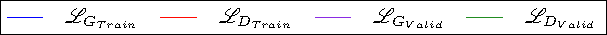
\includegraphics[width=0.6\linewidth]{{graphics/eval/cvgan_2/losses/loss_legend}.pdf}
	\end{subfigure}
	\vspace{0.01cm}
	
	\begin{subfigure}{0.32\linewidth}
	  \centering
		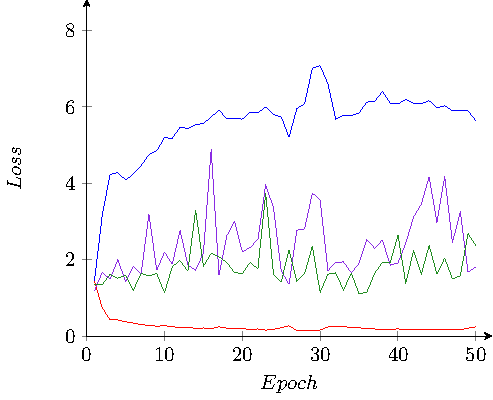
\includegraphics[width=\linewidth]{{graphics/eval/cvgan_2/losses/dfilter-32_ddropout-0.0_lambda-10_batchsize-64_learningrate-0.0002}.pdf}
		\vspace{-0.7cm}
		\caption{cf=32, dr=0.0, $\lambda$=10, bs=64, lr=2e-4}
		\label{subfig:cf=32-dr=0.0-l=10-bs=64-lr=2e-4-loss-1}
	\end{subfigure}
	\hfill
	\begin{subfigure}{0.32\linewidth}
	  \centering
		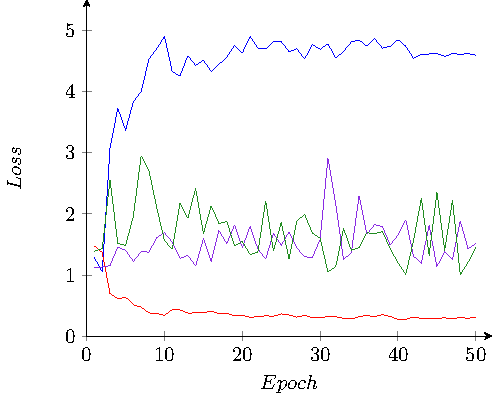
\includegraphics[width=\linewidth]{{graphics/eval/cvgan_2/losses/dfilter-16_ddropout-0.0_lambda-10_batchsize-64_learningrate-0.0002}.pdf}
		\vspace{-0.7cm}
		\caption{cf=16, dr=0.0, $\lambda$=10, bs=64, lr=2e-4}
		\label{subfig:cf=16-dr=0.0-l=10-bs=64-lr=2e-4-loss-1}
	\end{subfigure}
  \hfill
  \begin{subfigure}{0.32\linewidth}
    \centering
		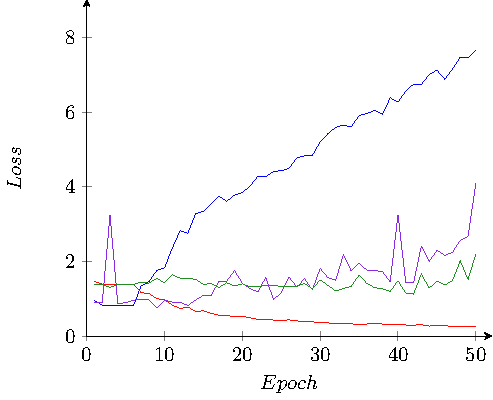
\includegraphics[width=\linewidth]{{graphics/eval/cvgan_2/losses/dfilter-16_ddropout-0.3_lambda-5_batchsize-64_learningrate-0.0002}.pdf}
		\vspace{-0.7cm}
		\caption{cf=16, dr=0.3, $\lambda$=5, bs=64, lr=2e-4}
		\label{subfig:cf=16-dr=0.3-l=5-bs=64-lr=2e-4-loss-1}
	\end{subfigure}
	
	\begin{subfigure}{0.32\linewidth}
	  \centering
		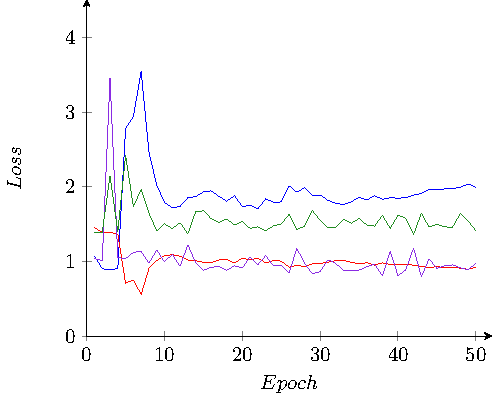
\includegraphics[width=\linewidth]{{graphics/eval/cvgan_2/losses/dfilter-16_ddropout-0.3_lambda-8_batchsize-64_learningrate-0.0002}.pdf}
		\vspace{-0.7cm}
		\caption{cf=16, dr=0.3, $\lambda$=8, bs=64, lr=2e-4}
		\label{subfig:cf=16-dr=0.3-l=8-bs=64-lr=2e-4-loss-1}
	\end{subfigure}
  \hfill
  \begin{subfigure}{0.32\linewidth}
	  \centering
		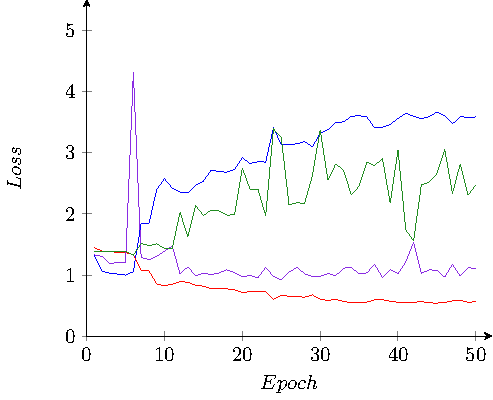
\includegraphics[width=\linewidth]{{graphics/eval/cvgan_2/losses/dfilter-16_ddropout-0.3_lambda-14_batchsize-64_learningrate-0.0002}.pdf}
		\vspace{-0.7cm}
		\caption{cf=16, dr=0.3, $\lambda$=14, bs=64, lr=2e-4}
		\label{subfig:cf=16-dr=0.3-l=14-bs=64-lr=2e-4-loss-1}
	\end{subfigure}
	\hfill
	\begin{subfigure}{0.32\linewidth}
	  \centering
		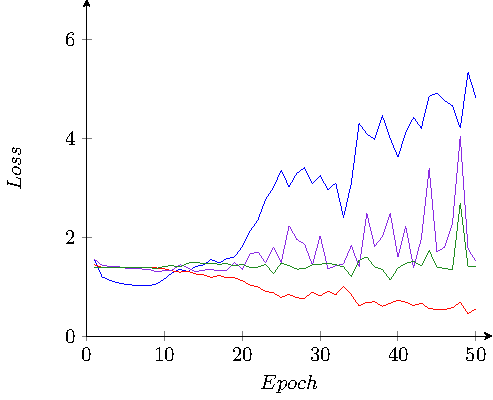
\includegraphics[width=\linewidth]{{graphics/eval/cvgan_2/losses/dfilter-16_ddropout-0.3_lambda-20_batchsize-64_learningrate-0.0002}.pdf}
		\vspace{-0.7cm}
		\caption{cf=16, dr=0.3, $\lambda$=20, bs=64, lr=2e-4}
		\label{subfig:cf=16-dr=0.3-l=20-bs=64-lr=2e-4-loss-1}
	\end{subfigure}  
		
	\caption[C-VGANs' training and validation losses over the epochs. (1)]{Training and validation losses ($\mathcal{L}$) over the epochs of generator ($G$) and discriminator ($D$) of C-VGAN for next-frame prediction using different hyperparameters. Note that higher losses do not necessarily imply a decrease in model quality; generator and discriminator should reach an equilibrium in their respective losses, with both of the models improving in parallel.}
	\label{fig:cvgan_losses_1}
\end{figure}

As a result, for the default configuration of the discriminator and with no dropout for each of its layers' outputs, not a single stable configuration was found. In every scenario, the discriminator overpowers the generator in the first 5--10 epochs, its loss converging towards $0$. Consequently the total generator loss quickly increases until its first loss term converges to its maximum value --- it is the negated second term of the discriminator loss term. The reconstruction loss term also falls into a local optimum and does not recover. This is to be expected as it is a known failure mode, in which the generator no longer improves in any way or actively degrades in quality (see Section \ref{sec:gans}). However this failure mode, as explained in the methodology in the previous section, can be quickly detected and training of such a C-VGAN configuration can be stopped early on, with the models being discarded. However for completeness sake, the default configuration was run for all $50$ epochs and its losses are depicted in Figure \ref{subfig:cf=32-dr=0.0-l=10-bs=64-lr=2e-4-loss-1}. It is to note, that in this configuration, while generator and discriminator training losses are both converging respectively, their validation losses behave differently: The discriminator loss on the validation dataset on every epoch is much higher and is fluctuating. This is an indicator for an overfitting discriminator model. This is further supported by the lower generator validation loss, as the discriminator can not distinguish synthetic and real videos extrapolated and drawn from the validation split, as it overfits the training split.

Consequently, attempts were made to impair the discriminator so the generator will manage to keep up with it. This was first done by reducing its convolutional filters on every layer ($cf$ parameter, see Section \ref{subsec:framework_cvgan}), so the discriminator is less able to contain every feature representation of real and synthetic videos. The result can be seen in Figure \ref{subfig:cf=16-dr=0.0-l=10-bs=64-lr=2e-4-loss-1}, with an overall smaller validation loss for both models. But the discriminator still overpowers the generator to some degree and overfits the training split, having a much higher validation loss than training loss. Configurations using the same parameters for the discriminator also behave that way, hence their training was stopped after epoch 10--20 when it became apparent. Next a dropout rate to the discriminator's layers was introduced ($dr$ parameter). And, in combination to the impairment in its convolutional filters, a stable equilibrium was found: Shown in Figure \ref{subfig:cf=16-dr=0.3-l=10-bs=64-lr=2e-4-loss-2}, after an initial spike in the generator loss accompanied by a drop in the discriminator's, the losses reach an equilibrium after epoch $20$. The validation split losses are also more stable, atleast for the discriminator. The generator validation loss has still an upward trend and when inspecting the generator training loss values closely, we noticed a small increase over the last epochs as well. Note this is not unusual, as the convergence for GANs is often not a stable state. The discriminator's feedback get less meaningful over time, causing the generator to optimize its parameters based on random feedback. 

\begin{figure}
  \centering
  
  \begin{subfigure}{\linewidth}
    \centering
		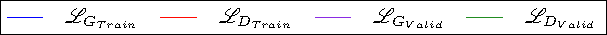
\includegraphics[width=0.6\linewidth]{{graphics/eval/cvgan_2/losses/loss_legend}.pdf}
	\end{subfigure}
	\vspace{0.01cm}
	
	\begin{subfigure}{0.32\linewidth}
	  \centering
		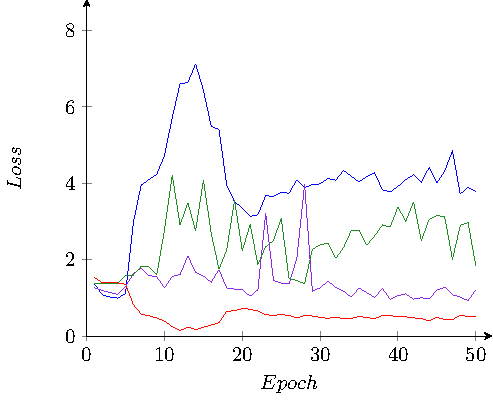
\includegraphics[width=\linewidth]{{graphics/eval/cvgan_2/losses/dfilter-16_ddropout-0.3_lambda-10_batchsize-256_learningrate-0.0004}.pdf}
		\vspace{-0.7cm}
		\caption{cf=16, dr=0.3, $\lambda$=10, bs=256, lr=4e-4}
		\label{subfig:cf=16-dr=0.3-l=10-bs=256-lr=4e-4-loss-2}
	\end{subfigure}
	\hfill
	\begin{subfigure}{0.32\linewidth}
	  \centering
		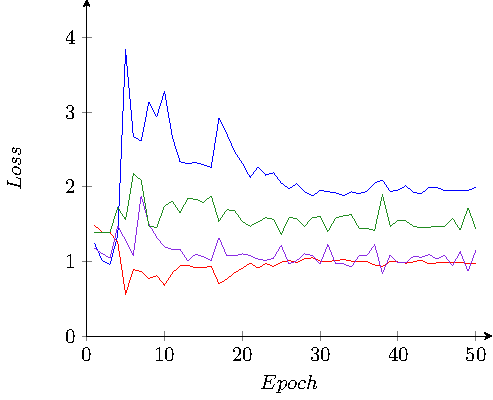
\includegraphics[width=\linewidth]{{graphics/eval/cvgan_2/losses/dfilter-16_ddropout-0.3_lambda-10_batchsize-128_learningrate-0.00028}.pdf}
		\vspace{-0.7cm}
		\caption{cf=16, dr=0.3, $\lambda$=10, bs=128, lr=2.8e-4}
		\label{subfig:cf=16-dr=0.3-l=10-bs=128-lr=2.8e-4-loss-2}
	\end{subfigure}
	\hfill
	\begin{subfigure}{0.32\linewidth}
	  \centering
		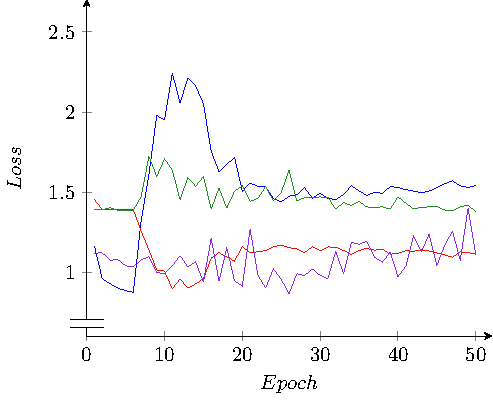
\includegraphics[width=\linewidth]{{graphics/eval/cvgan_2/losses/dfilter-16_ddropout-0.3_lambda-10_batchsize-64_learningrate-0.0002}.pdf}
		\vspace{-0.7cm}
		\caption{cf=16, dr=0.3, $\lambda$=10, bs=64, lr=2e-4}
		\label{subfig:cf=16-dr=0.3-l=10-bs=64-lr=2e-4-loss-2}
	\end{subfigure}
	
	\begin{subfigure}{0.32\linewidth}
	  \centering
		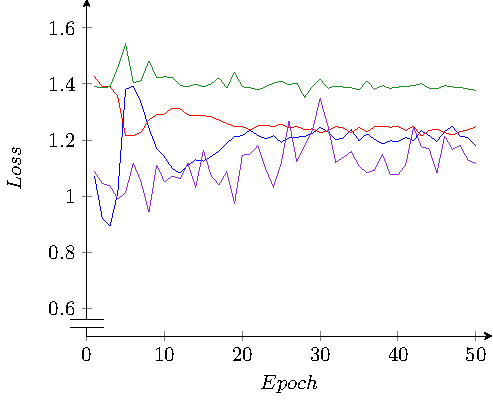
\includegraphics[width=\linewidth]{{graphics/eval/cvgan_2/losses/dfilter-16_ddropout-0.3_lambda-10_batchsize-32_learningrate-0.0002}.pdf}
		\vspace{-0.7cm}
		\caption{cf=16, dr=0.3, $\lambda$=10, bs=32, lr=2e-4}
		\label{subfig:cf=16-dr=0.3-l=10-bs=32-lr=2e-4-loss-2}
	\end{subfigure}
	\hfill
	\begin{subfigure}{0.32\linewidth}
	  \centering
		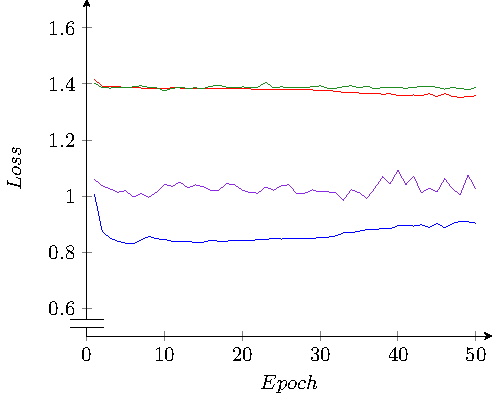
\includegraphics[width=\linewidth]{{graphics/eval/cvgan_2/losses/dfilter-16_ddropout-0.3_lambda-10_batchsize-16_learningrate-0.0002}.pdf}
		\vspace{-0.7cm}
		\caption{cf=16, dr=0.3, $\lambda$=10, bs=16, lr=2e-4}
		\label{subfig:cf=16-dr=0.3-l=10-bs=16-lr=2e-4-loss-2}
	\end{subfigure}
	\hfill
	\begin{subfigure}{0.32\linewidth}
	  \centering
		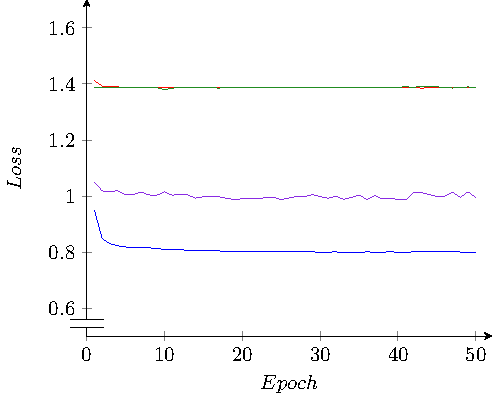
\includegraphics[width=\linewidth]{{graphics/eval/cvgan_2/losses/dfilter-16_ddropout-0.3_lambda-10_batchsize-8_learningrate-0.0002}.pdf}
		\vspace{-0.7cm}
		\caption{cf=16, dr=0.3, $\lambda$=10, bs=8, lr=2e-4}
		\label{subfig:cf=16-dr=0.3-l=10-bs=8-lr=2e-4-loss-2}
	\end{subfigure}
			
	\caption[C-VGANs' training and validation losses over the epochs. (2)]{Training and validation losses ($\mathcal{L}$) over the epochs of generator ($G$) and discriminator ($D$) of C-VGAN for next-frame prediction using different hyperparameters. Note that higher losses do not necessarily imply a decrease in model quality; generator and discriminator should reach an equilibrium in their respective losses, with both of the models improving in parallel.}
	\label{fig:cvgan_losses_2}
\end{figure}

\begin{figure}
  \centering

	\begin{subfigure}{\textwidth}
		\centering
		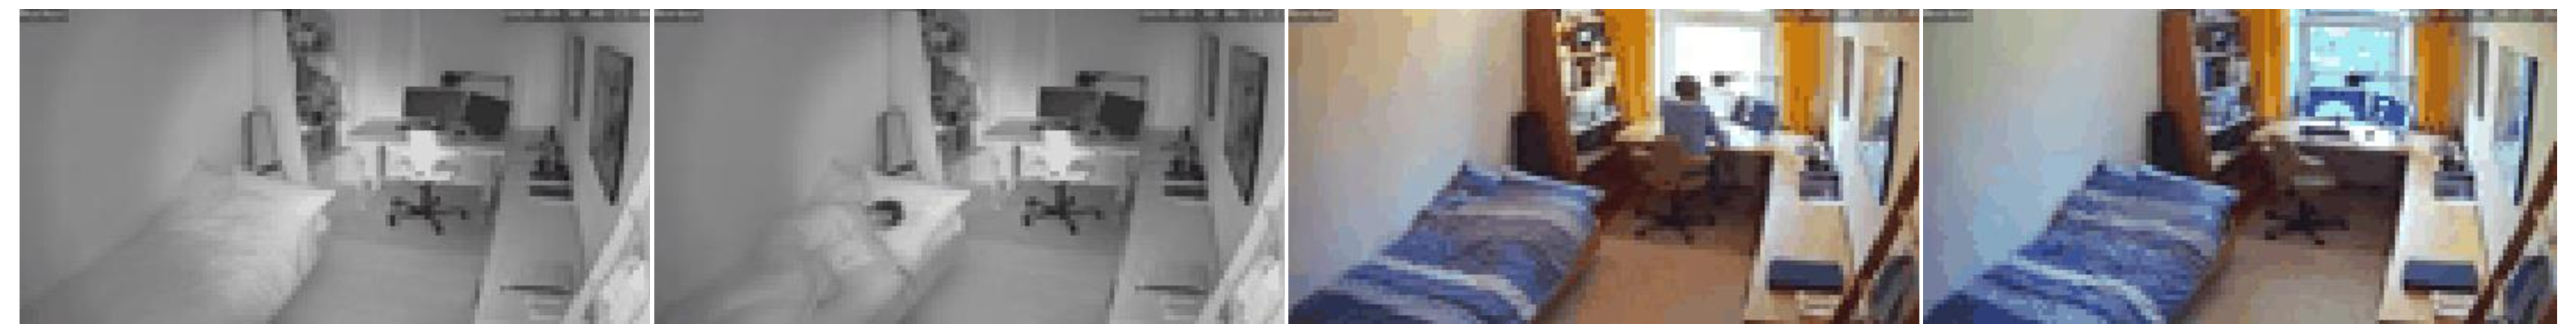
\includegraphics[width=\textwidth]{graphics/eval/cvgan_2/qual_basic/actual/actual.pdf}
	  \caption{Actual next frames.}
	  \label{subfig:cvgan_comparison_lambda}
	\end{subfigure}

	\begin{subfigure}{\textwidth}
		\centering
		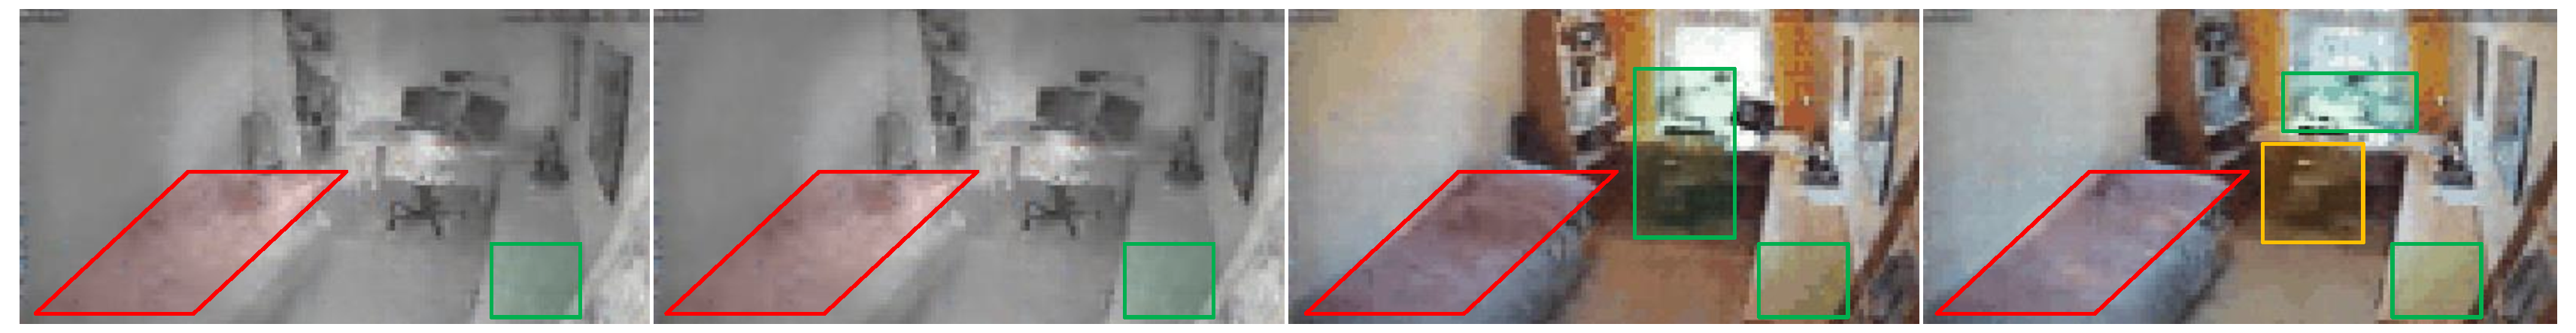
\includegraphics[width=\textwidth]{graphics/eval/cvgan_2/qual_basic/dfilter-16_ddropout-0.3_lambda-5_batchsize-64_learningrate-0.0002/predicted.pdf}
	  \caption{cf=16, dr=0.3, $\lambda$=5, bs=64, lr=2e-4}
	  \label{subfig:l5-comp-1}
	\end{subfigure}

	\begin{subfigure}{\textwidth}
		\centering
		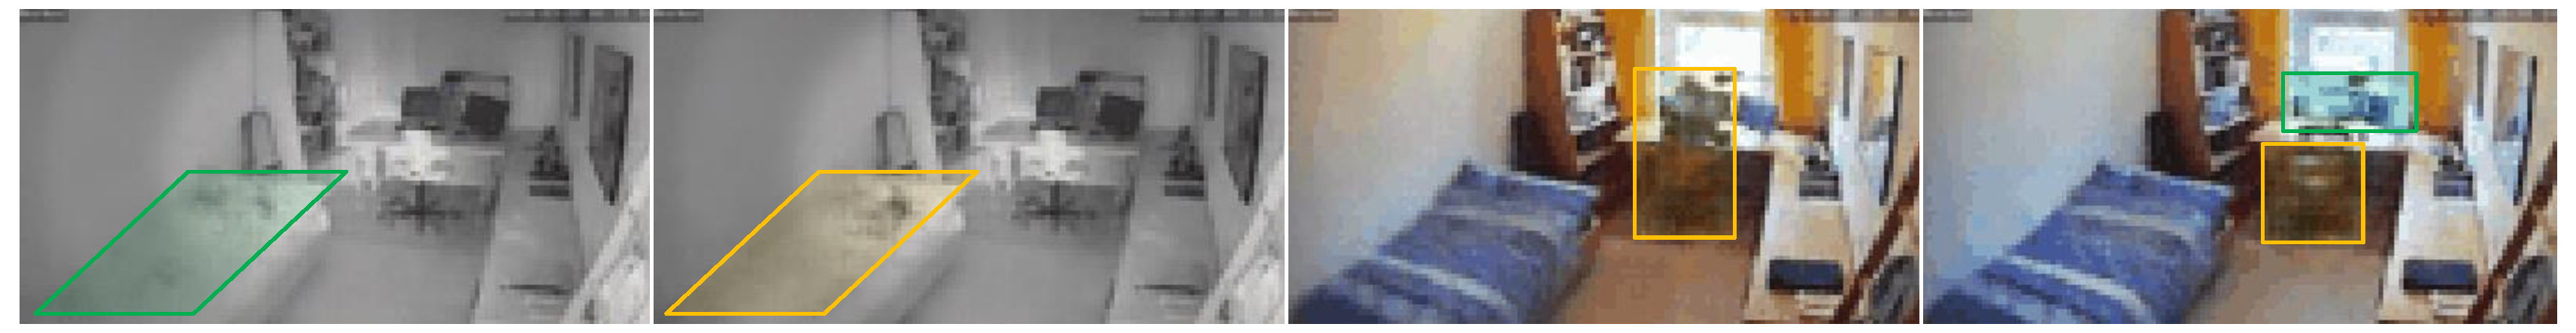
\includegraphics[width=\textwidth]{graphics/eval/cvgan_2/qual_basic/dfilter-16_ddropout-0.3_lambda-8_batchsize-64_learningrate-0.0002/predicted.pdf}
	  \caption{cf=16, dr=0.3, $\lambda$=8, bs=64, lr=2e-4}
	  \label{subfig:l8-comp-1}
	\end{subfigure}

	\begin{subfigure}{\textwidth}
		\centering
		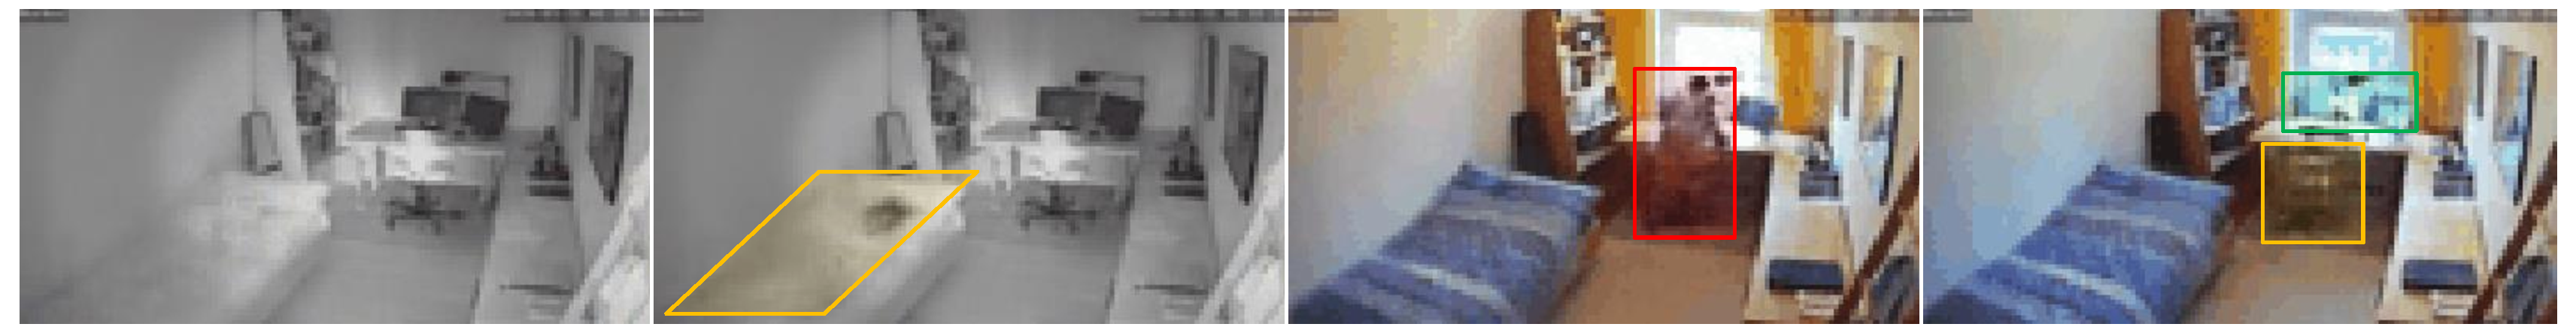
\includegraphics[width=\textwidth]{graphics/eval/cvgan_2/qual_basic/dfilter-16_ddropout-0.3_lambda-10_batchsize-64_learningrate-0.0002/predicted.pdf}
	  \caption{cf=16, dr=0.3, $\lambda$=10, bs=64, lr=2e-4}
	  \label{subfig:l10-comp-1}
	\end{subfigure}

	\begin{subfigure}{\textwidth}
		\centering
		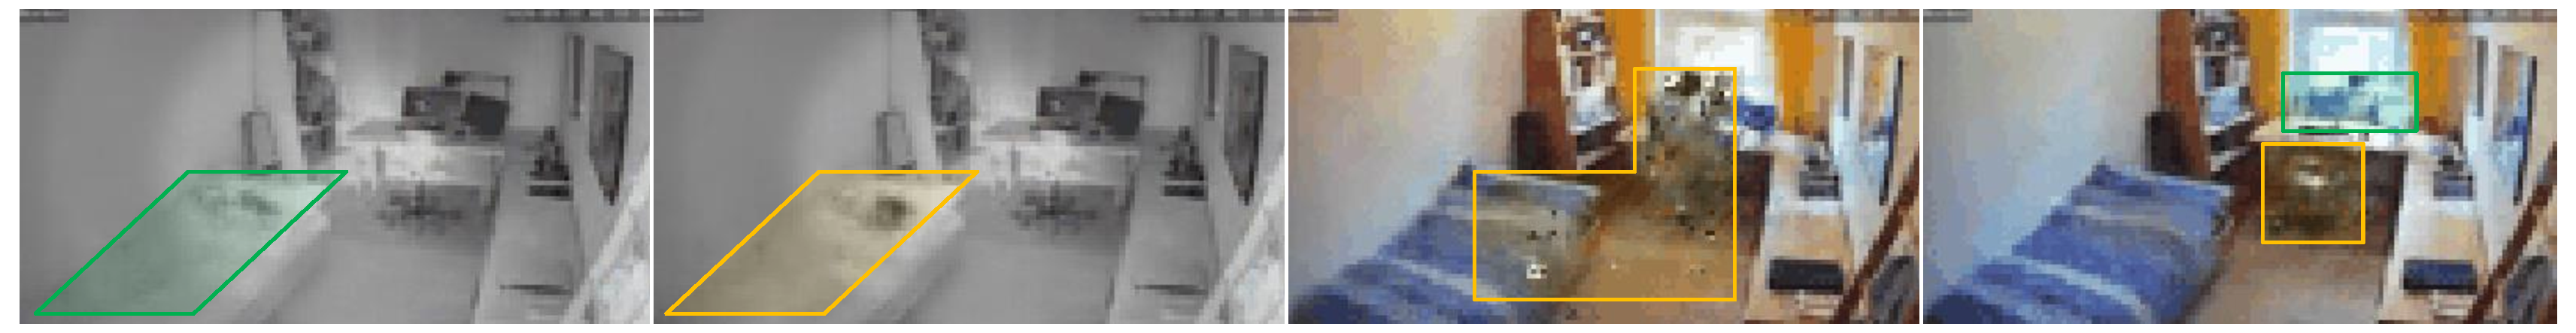
\includegraphics[width=\textwidth]{graphics/eval/cvgan_2/qual_basic/dfilter-16_ddropout-0.3_lambda-14_batchsize-64_learningrate-0.0002/predicted.pdf}
	  \caption{cf=16, dr=0.3, $\lambda$=14, bs=64, lr=2e-4}
	  \label{subfig:l14-comp-1}
	\end{subfigure}
	
	\caption[Qualitative comparison between different C-VGAN models. (1)]{Comparison between the actual next frames of video clips (a) and their respective predictions by C-VGAN models that were trained using different weights ($\lambda$) for their reconstruction loss term. Marked in red one can see how different object patterns are collapsed into the same pattern. Omitted or hallucinated objects are colored in green, and objects that lack detail or are not fully constructed are marked yellow.}
	\label{fig:cvgan_comparison_lambda}
\end{figure}

Following the discovery of a configuration that accomplishes an equilibrium, attempts were made to fine tune the parameter $\lambda$, regulating how much the input frames determine the output, but this either ruined the balance of the two models --- see Figure \ref{fig:cvgan_losses_1} for some of the attempt's results, or worsened the quality of the output. The latter will be further assessed during the presentation of the qualitative evaluation. Tuning the batch size however produced mixed results, depicted in Figure \ref{fig:cvgan_losses_2}: Increasing it and with it the learning rate, on one hand sped up training, but on the other resulted in generally higher overall losses. Although this is not necessarily bad as long as models improve in parallel, it requires further qualitative evaluation of the model's outputs. Meanwhile, when greatly decreasing the batch size but keeping the learning rate fixed, convergence of the losses is not only faster but extremely stable. This is not only for the case for the training losses but also for the validation split. In case of the discriminator, validation and training loss are practically identical when using a batch size of $16$ and $8$, with a slight upward and downward trend for the generator and discriminator training losses after epoch $30$, respectively, for a batch size of $16$. See Figure \ref{subfig:cf=16-dr=0.3-l=10-bs=16-lr=2e-4-loss-2} and \ref{subfig:cf=16-dr=0.3-l=10-bs=8-lr=2e-4-loss-2}. This is a sign for great generalization. For the generator, validation loss is still higher, which means it is not able to reconstruct unknown frames as well as ones that were witnessed during training. Even so, both generator losses are still lower with smaller training batches than when using any other configuration. This confirms our hypothesis from Section \ref{subsec:framework_cvgan}, that while higher batch sizes are a good tool to help with generalization and drown out sparse anomalies in the training data set, they are also hurting the model to learn less frequently occurring object patterns. In addition, smaller batches also seem to help the generator to keep up with its counterpart: Giving the discriminator less examples per step is an indirect impairment to its training process, because the model is smaller and can more quickly adapt to the observations witnessed in a step. Limiting that is especially crucial in the initial epochs, because this is when the generator loss peaks in other configurations before converging to a lower value. Preventing this early overpowering, that might put the generator into a bad local minimum, also improves the generator's overall quality.

Finally for the configurations that are still in a balance after $50$ epochs there could be better results if one were to train those further. Nonetheless for the scope of this evaluation and due to the high time cost, training was stopped at that point with the option to evaluate the other models from their earlier epochs before their respective loss equilibria were lost and they had regressed in quality.

\paragraph{Qualitative Results}

\begin{figure}
  \centering

	\begin{subfigure}{\textwidth}
		\centering
		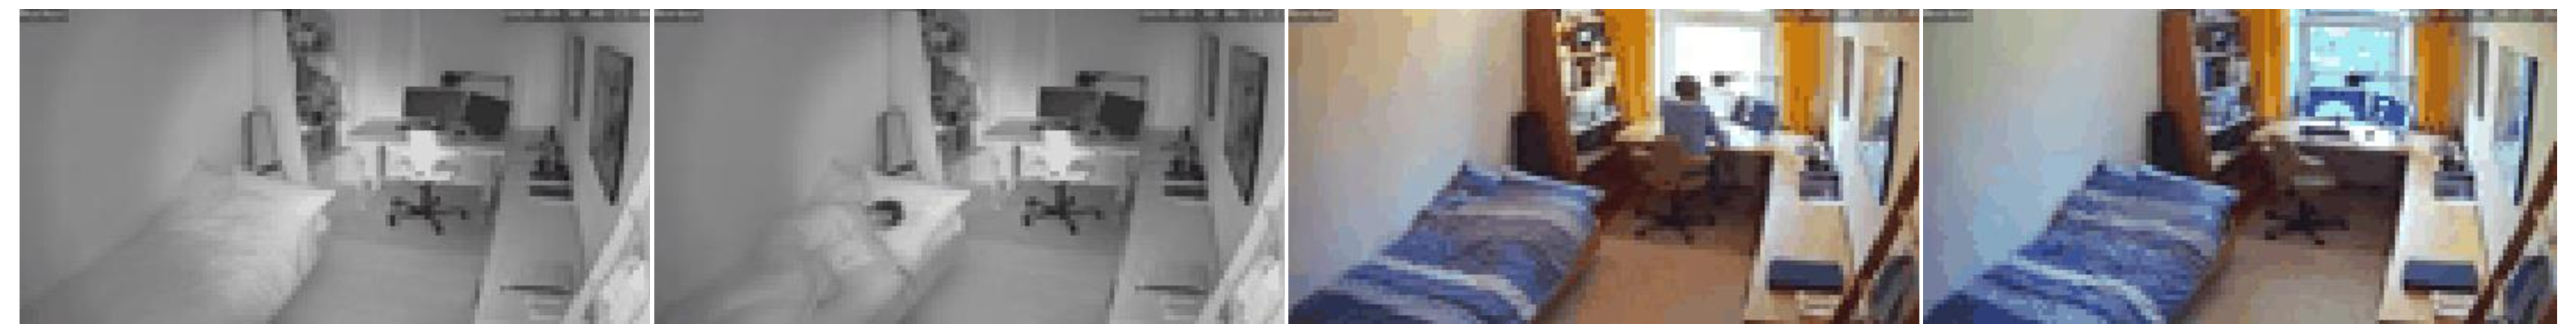
\includegraphics[width=\textwidth]{graphics/eval/cvgan_2/qual_basic/actual/actual.pdf}
	  \caption{Actual next frames.}
	  \label{subfig:cvgan_comparison_bs}
	\end{subfigure}
	
	\begin{subfigure}{\textwidth}
	  \centering
		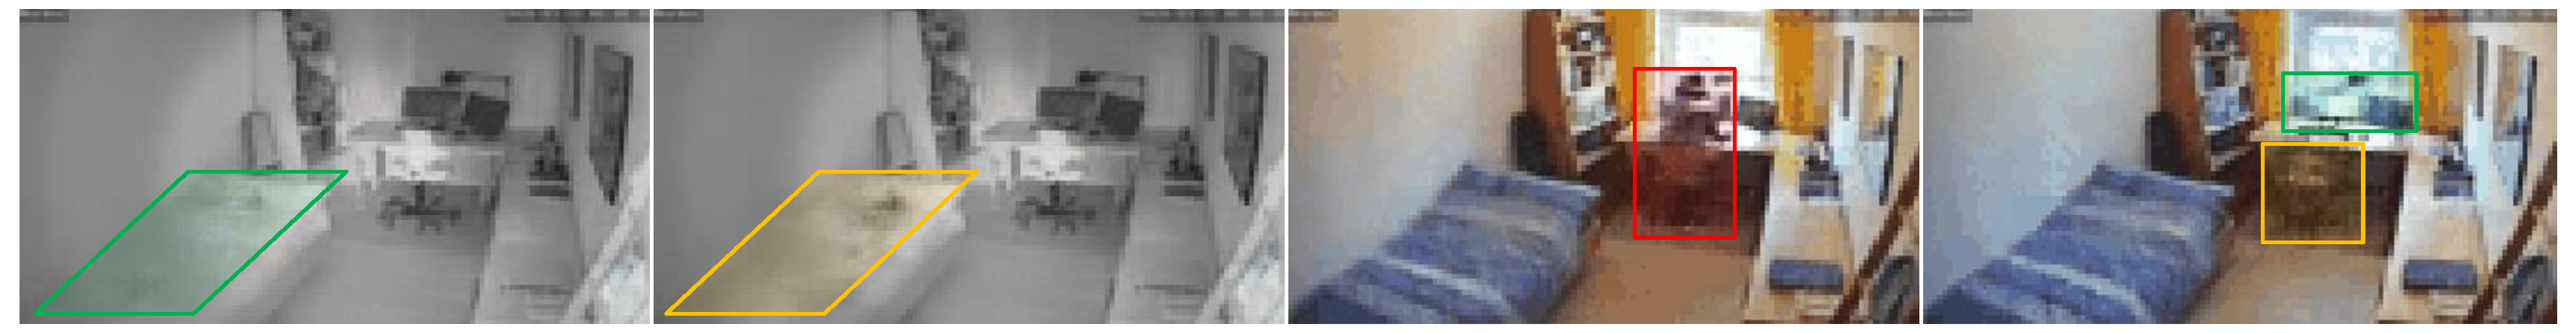
\includegraphics[width=\textwidth]{graphics/eval/cvgan_2/qual_basic/dfilter-16_ddropout-0.3_lambda-10_batchsize-128_learningrate-0.00028/predicted.pdf}
		\caption{cf=16, dr=0.3, $\lambda$=10, bs=128, lr=2.8e-4}
		\label{subfig:bs128-comp-2}
	\end{subfigure}

	\begin{subfigure}{\textwidth}
		\centering
		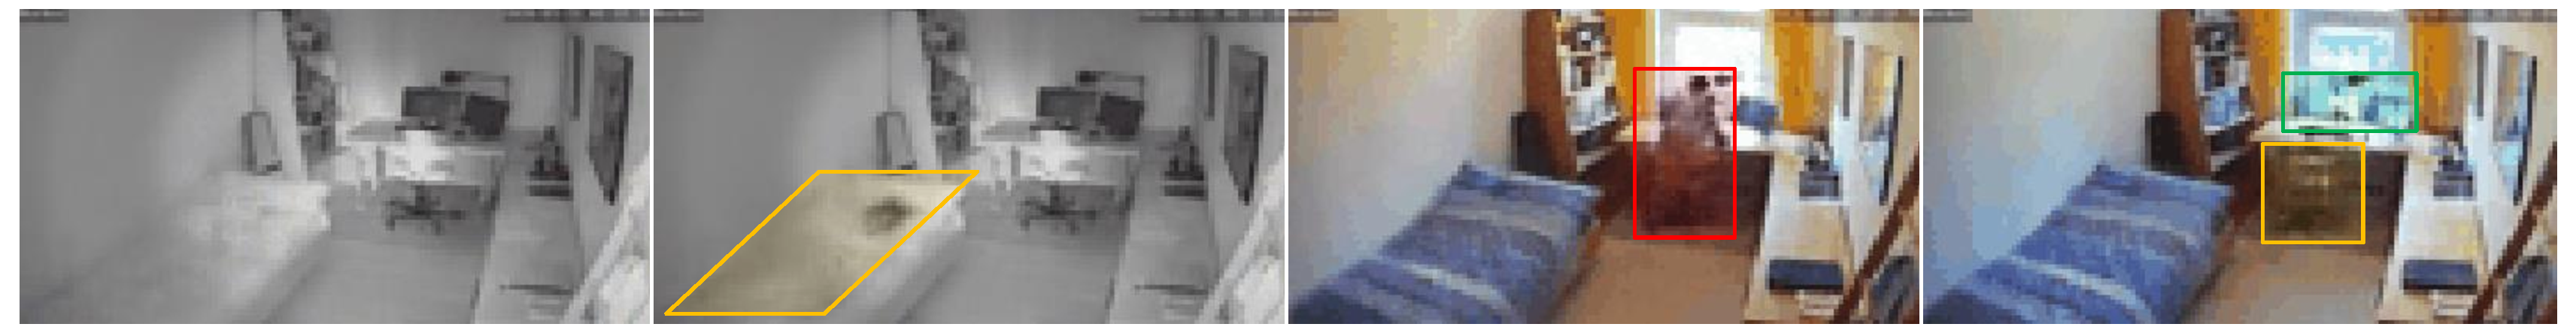
\includegraphics[width=\textwidth]{graphics/eval/cvgan_2/qual_basic/dfilter-16_ddropout-0.3_lambda-10_batchsize-64_learningrate-0.0002/predicted.pdf}
	  \caption{cf=16, dr=0.3, $\lambda$=10, bs=64, lr=2e-4}
	  \label{subfig:bs64-comp-2}
	\end{subfigure}

	\begin{subfigure}{\textwidth}
		\centering
		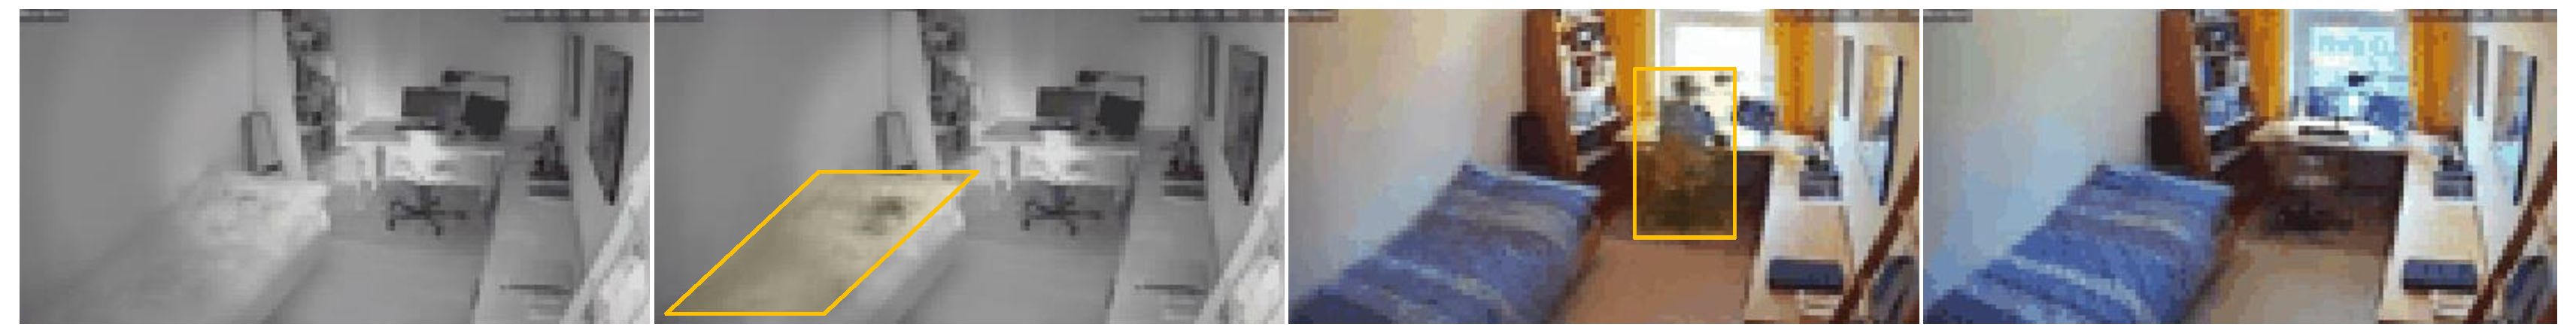
\includegraphics[width=\textwidth]{graphics/eval/cvgan_2/qual_basic/dfilter-16_ddropout-0.3_lambda-10_batchsize-32_learningrate-0.0002/predicted.pdf}
	  \caption{cf=16, dr=0.3, $\lambda$=10, bs=32, lr=2e-4}
	  \label{subfig:bs32-comp-2}
	\end{subfigure}

	\begin{subfigure}{\textwidth}
		\centering
		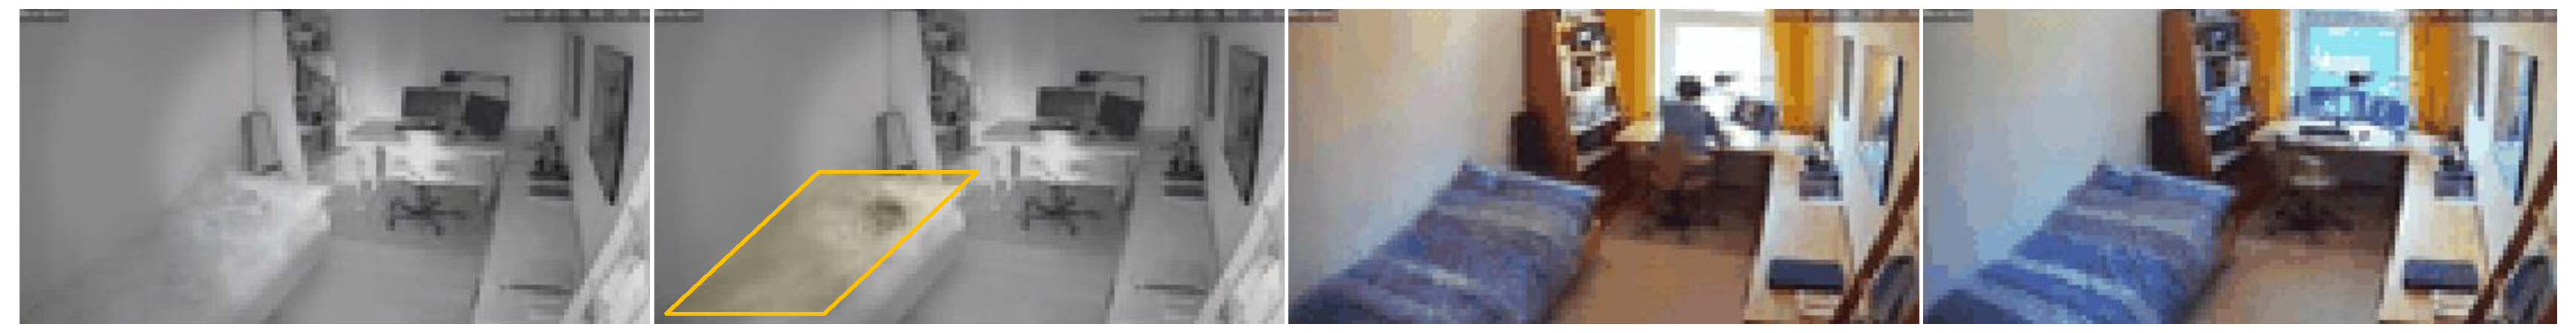
\includegraphics[width=\textwidth]{graphics/eval/cvgan_2/qual_basic/dfilter-16_ddropout-0.3_lambda-10_batchsize-16_learningrate-0.0002/predicted.pdf}
	  \caption{cf=16, dr=0.3, $\lambda$=10, bs=16, lr=2e-4}
	  \label{subfig:bs16-comp-2}
	\end{subfigure}
	
	\caption[Qualitative comparison between different C-VGAN models. (2)]{Comparison between the actual next frames of video clips (a) and their respective predictions by C-VGAN models that were trained using different batch sizes ($bs$). Marked in red one can see how different object patterns are collapsed into the same pattern. Omitted or hallucinated objects are colored in green, and objects that lack detail or are not fully constructed are marked yellow.}
	\label{fig:cvgan_comparison_bs}
\end{figure}

Since none of the configurations in which the discriminator was not impaired proved to be stable, they are not included in the qualitative assessment. Overall, their reconstructed and predicted frames were of poor quality and contained a lot of noise. They are not alone in this, as any changes to the reconstruction loss term weight ($\lambda$) also worsened the quality of the output video clips. Shown in Figure \ref{fig:cvgan_comparison_lambda}, one can see some of these configurations making next-frame predictions on the test split of the training data set. For low values of $\lambda$, hallucinations and omissions of object patterns are common, same as the collapsing of different input videos into the same outputs. Although this could still be used for IFTM if normal instances are collapsed into the same outputs while anomalous ones are not, this does not meet the requirement for a next-frame forecasting model. In contrast, giving the reconstruction loss too much weight compared to the prediction of the 8th frame, worsens its quality drastically. Depicted in Figure \ref{subfig:l14-comp-1}, the model even hallucinates a person lying in the bed when using a higher reconstruction loss weight and inserts gray noise into videos during the day. One can assume that features from observations from the night bleed into that output, causing that noise. This gets worse as the number of epochs increase, which matches the results for the model loss progression from the previous section. For the default reconstruction loss term weight ($\lambda$=10), there are fewer errors in the object patterns, with the exception of the substitution of the person's clothing and the change in posture (marked in red in Figure \ref{subfig:l10-comp-1}). This is also hint of some form of output collapse, and makes such a prediction model insufficient. Finally in all of these configurations, the computer displays on the desk often merge with the window during the day, having no clear boundary between them and the light that emits from the outside. 

The last issues disappear, along hallucination issues for the test split, once the batch size is decreased, as shown in Figure \ref{fig:cvgan_comparison_bs}: Starting with a batch size of $32$, the clothing of the person gets successfully reconstructed along with their posture, and beyond a batch size of $16$, the object pattern of the person is also indistinguishable from the one in the actual frame. The light from the window is also more true to the ground truth. Yet some inaccuracies and noise remain; for example no matter the configuration the person lying in bed is always blurry. The same is the case for the dynamic content of the computer displays on the desk, although from our point of view the latter difference is negligible (see Figure \ref{subfig:bs16-comp-2}).

\begin{figure}
  \centering

	\begin{subfigure}{\textwidth}
		\centering
		\includegraphics[width=0.9\textwidth]{graphics/eval/cvgan_2/qual_prediction/real/normal.pdf}
	  \caption{Actual next frames.}
	  \label{subfig:cvgan_prediction_normal}
	\end{subfigure}
	
	\begin{subfigure}{\textwidth}
	  \centering
		\includegraphics[width=0.9\textwidth]{graphics/eval/cvgan_2/qual_prediction/cvgan_2_dfilter-16_ddropout-0.3_lambda-10_batchsize-128_learningrate-0.000282842712474619_epochs-0050/normal.pdf}
		\caption{cf=16, dr=0.3, $\lambda$=10, bs=128, lr=2.8e-4}
		\label{subfig:bs128-pred-n}
	\end{subfigure}	
	
	\begin{subfigure}{\textwidth}
	  \centering
		\includegraphics[width=0.9\textwidth]{graphics/eval/cvgan_2/qual_prediction/cvgan_2_dfilter-16_ddropout-0.3_lambda-10_batchsize-8_learningrate-0.0002_epochs-0050/normal.pdf}
		\caption{cf=16, dr=0.3, $\lambda$=10, bs=8, lr=2e-4}
		\label{subfig:bs8-pred-n}
	\end{subfigure}
	
	\caption[Prediction error heat maps for normal frames predicted by C-VGANs.]{Comparison between the actual next frames (a) and predictions by two differently configured C-VGAN models, further illustrated and dissected as heat maps of the pixel-wise mean absolute error. Note that the overall prediction error for these frames should be minimal, as they only contain assumed normal object patterns (see Section \ref{subsec:dataset_properties}).}
	\label{fig:cvgan_prediction_normal}
\end{figure}

\begin{figure}
  \centering

	\begin{subfigure}{\textwidth}
		\centering
		\includegraphics[width=0.9\textwidth]{graphics/eval/cvgan_2/qual_prediction/real/anomalous.pdf}
	  \caption{Actual next frames.}
	  \label{subfig:cvgan_prediction_anomalous}
	\end{subfigure}
	
  \begin{subfigure}{\textwidth}
	  \centering
		\includegraphics[width=0.9\textwidth]{graphics/eval/cvgan_2/qual_prediction/cvgan_2_dfilter-16_ddropout-0.3_lambda-10_batchsize-128_learningrate-0.000282842712474619_epochs-0050/anomalous.pdf}
		\caption{cf=16, dr=0.3, $\lambda$=10, bs=128, lr=2.8e-4}
		\label{subfig:bs128-pred-a}
	\end{subfigure}	
	
	\begin{subfigure}{\textwidth}
	  \centering
		\includegraphics[width=0.9\textwidth]{graphics/eval/cvgan_2/qual_prediction/cvgan_2_dfilter-16_ddropout-0.3_lambda-10_batchsize-8_learningrate-0.0002_epochs-0050/anomalous.pdf}
		\caption{cf=16, dr=0.3, $\lambda$=10, bs=8, lr=2e-4}
		\label{subfig:bs8-pred-a}
	\end{subfigure}
	
	\caption[Prediction error heat maps for anomalous frames predicted by C-VGANs.]{Comparison between the actual next frames (a) and predictions by two differently configured C-VGAN models, further illustrated and dissected as heat maps of the pixel-wise mean absolute error. Note that these frames are considered anomalous in nature (see Section \ref{subsec:dataset_properties}), so for the purpose of IFTM, the models must be unable to predict these as accurately as normal frames.}
		\label{fig:cvgan_prediction_anomalous}
\end{figure}

The benefit of smaller batches during training becomes even more apparent, when evaluating some of the models based on their prediction quality on the evaluation data set. In Figure \ref{fig:cvgan_prediction_normal}, one can see three frames and how they were predicted by two configurations using different batch sizes. These frames are part of a larger event in which the person moves towards the desk and sits down. One can see how a larger batch size is unable to model any of the motion dynamics properly, trying to hallucinate a sitting person at the desk in the second and third depicted frame, but even failing to do that. A batch size of $8$ on the other hand manages to model the initial movement, before failing to accurately model the sitting down motion pattern. It can be assumed that the model lacked many diverse observations in which these object patterns occur, so it naturally struggles to make reconstructions and predictions for such rare events. Yet the heat map shows that the object with the motion pattern is not driving the over all prediction error for C-VGAN with bs=$8$, not unlike for a batch size of $128$. 

When giving both configurations anomalous events from the evaluation data set however, one notices that a smaller batch size also helps with the generalization and prediction of these anomalous frames, which is detrimental to our use case: In the first frame of Figure \ref{fig:cvgan_prediction_anomalous}, the computer displays are turned off while the person sits at the desk for a while --- a collective anomaly, but besides hallucinations of a bit of light on one of the displays for the model that was trained using the larger batch size, there are not any noticeable prediction errors showing on the heat map for that event. On the other hand, when anomalous object patterns are less local and occur in larger portions of the scene, both models successfully fail to model them properly. As seen in the heat maps of the second and third example, their errors are mostly the same, with the generator being able to partially omit the person sitting in the middle of the room.

Nonetheless, the first anomalous example in the figure is a symptom of a larger problem when training video generation models not only for prediction, but to only be able to model the normal state of the system, while being unable to make predictions during anomalous events. For the latter, our models seem to be able to generalize the future well enough, so that this particular series of anomalous frames can be accurately predicted. And these predictions even have a smaller error than some of the normal examples depicted in Figure \ref{fig:cvgan_prediction_normal}. Then, there are also prediction errors occurring in unexpected places: The outlines of the pillows on the bed, but also the shelf in the background, some papers on the lowboard, and the ladder in the right foreground are visible in all the depicted error heat maps, both anomalous frames and normal. This is an indicator for an occurrence of output collapse, because the models, as explained in our methodology in the previous section, are only trained with $6$ days of data. This in the worst case, gives the models only $6$ different positions for the pillows, as the bed is only made once per day. Unlike with various other object patterns and for the person interacting with the room, any new position of these pillows either has to be reconstructed or is collapsed into one of the known object patterns. The same is the case for the papers on the lowboard and the other examples listed above, creating a constant noise of falsely predicted normal object patterns in each frame that is not from the training split. Note that these errors can be safely ignored, when using C-VGAN for next-frame predictions, as these errors are barely noticeable by a human. But when using such a model for IFTM and VAD, these static errors for normal object patterns in a scene will skew with the classification results, as it gives all incoming frames a higher anomaly score no matter the true label. This challenge and how it can be solved to improve on the quality of our anomaly detection approach for video, will be discussed after the VAD evaluation results have been presented in the following section.



% Anomaly Detection Evaluation
\section{Anomaly Detection for Video using IFTM} \label{sec:vad_eval}

Loading C-VGAN models for next-frame video prediction into the adapted IFTM framework presented in Section \ref{sec:vad}, the ADS can then be evaluated on its performance for VAD. As mentioned throughout the previous chapter, the modified version of IFTM has no additional hyperparameters that need tuning: The identity function (IF) is the fully trained prediction generator model of C-VGAN loaded from disk, while the threshold model (TM) can be computed using the training data set, the IF, and the prediction error function. Hence in this Section, C-VGAN generators that were evaluated in the prior section are taken as they are. To assess IFTM with different underlying prediction models, quantitative metrics were chosen as the main tool for evaluation. These are provided first, with an explanation of their meaning. The resulting anomaly detection metrics for the different IFTM configurations is then presented afterwards.


% Anomaly Detection Evaluation Methods
\subsection{Evaluation Method} \label{subsec:vad_eval_method} % 3 Pages

\paragraph{Confusion Matrix and Derived Metrics}

\begin{table}
	\centering
	\begin{tabular}{| c | c | c | c |}
	\toprule
	\multicolumn{2}{| c |}{\multirow{2}{*}{}} 	  & \multicolumn{2}{ c |}{\textit{\textbf{Actual}}} \\
	\cmidrule{3-4}
	\multicolumn{2}{| c |}{} 						          & \textbf{Anomaly} & \textbf{Normal} \\
	\midrule
	\multirow[c]{2}{*}{\textit{\textbf{Predicted}}}& \textbf{Anomaly} 	& True Positive (TP)  & False Positive (FP)	\\
	\cmidrule{2-4}
												  & \textbf{Normal} 	& False Negative (FN) & True Negative (TN)	\\
	\bottomrule
	\end{tabular}
	\caption[Confusion matrix for anomaly detection evaluation.]{Binary confusion matrix for anomaly detection evaluation.}
	\label{tab:confusion_matrix}
\end{table}

Our adapted version of IFTM labels every frame in a video stream in binary fashion (0=normal and 1=anomalous). And, as explained in Section \ref{subsec:framework_iftm} and \ref{subsec:postprocessing}, these predicted labels can then logged and be used to quantitatively evaluate different model configurations. Using our labeled evaluation data set presented in detail in Section \ref{sec:dataset}, we can compare the true label of each frame to the one predicted by a model. Doing this over the entire data set and aggregating the results, a confusion matrix for all existing samples and their classes can be constructed, as shown in Table \ref{tab:confusion_matrix}: A special kind of contingency table, the rows of the matrix represent the instances in the predicted classes, while the columns are the instances in the actual classes. Given it is a binary matrix, there are four outcomes: If an anomalous frame was labeled as an anomaly, it would count as a true positive, but if it was predicted to be normal, it would be a false negative, i.e. an omitted anomaly. Vice versa, if a normal frame was classified as an anomaly, it would be a false positive --- a false alarm. A true negative would be the same frame labeled as normal.

\begin{table}
	\centering
	\begin{tabular}{ | L{4.7cm} | l |}
	\toprule
	\textbf{Metric} & \textbf{Derivation from Confusion Matrix} \\
	\midrule
	True Positive Rate \quad \quad 
	(Recall, Sensitivity) & $TPR = \frac{TP}{TP + FN} = 1 - FNR$ \\[1ex]  %recall = tp / (tp + fn)
	True Negative Rate 
	(Specificity)  & $TNR = \frac{TN}{TN + FP} = 1 - FPR$ \\[1ex]  %tnr = tn / (tn + fp)
	Positive Predictive Value 
	(Precision)    & $PPV = \frac{TP}{TP + FP}$ 	        \\[1ex]  %precision = tp / (tp + fp)
	Negative Predictive Value
                 & $NPV = \frac{TN}{TN + FN}$ 	        \\[1ex]  %npv = tn / (tn + fn)
	False Positive Rate \quad \quad 
	(Fall-Out)     & $FPR = \frac{FP}{FP + TN} = 1 - TNR$ \\[1ex]  %fpr = fp / (fp + tn)
	False Negative Rate \quad \quad 
	 (Miss Rate)   & $FNR = \frac{FN}{FN + TP} = 1 - TPR$ \\[1ex]  %fnr = fn / (fn + tp)
	Accuracy       & $Acc = \frac{TP + TN}{TP + TN + FP + FN} = \frac{TP + TN}{total}$ \\[1ex]  %accuracy = (tp + tn) / self.total
	F-Measure      & $F_1 = \frac{2 \cdot TP}{2 \cdot TP + FP + TN} = \frac{2}{TPR^{-1}+PPV^{-1}}$ 	\\[1ex]  %f1 = 2 * tp / (2 * tp + fp + fn)
	\bottomrule
	\end{tabular}
	\caption[Anomaly detection evaluation metrics.]{Anomaly detection evaluation metrics, derived from the binary confusion matrix. Often used aliases for the metrics are given in parenthesis.}
	\label{tab:eval_metrics}
\end{table}

Using the aggregated counts of each outcome, one can derive many commonly used evaluation metrics from it. For the quantitative evaluation of IFTM for VAD, the eight metrics presented in Table \ref{tab:eval_metrics} were selected: First, it is important to evaluate how many of the actual normal and anomalous samples were correctly predicted by the detection model. Recall and specificity represent these two rates. Their direct counterparts, the rates anomalies and normal data points are labeled incorrectly are redundant but helpful to inspect the rate of false alarms and omitted anomalies directly. This is especially useful in case a model is very sensitive: Detecting nearly every frame as an anomaly would result in both a high recall and a high false alarm rate (fall-out). Next, positive and negative predictive value represent how many of the instances of their predicted respective classes actually belong to their class. But these two metrics can also be deceiving, especially in unbalanced data sets. For example, roughly $30\%$ of our evaluation data set are anomalies, as presented in detail in Section \ref{sec:dataset}. Labeling all of the data set's samples as normal would result in a fairly high negative predictive value ($70\%$). At the same time, a high positive predictive value can be achieved by exclusively labeling a few actual anomalous data points as anomalies, while still classifying most actual anomalies incorrectly. 

There are metrics which try to aggregate the information of the confusion matrix further: Accuracy depicts the overall rate of correct predictions. Although it has similar issues as the metrics above if the data set is unbalanced --- labeling one class mostly correctly while ignoring the other can still achieve a high accuracy under those circumstances, it can still be used as an additional indicator for a good anomaly detection model. In addition, we chose the F-measure as our last evaluation metric, which combines recall and precision into a single value using the harmonic mean. This metric would be lower in case a model classified all samples as anomalies for example, resulting in a high recall, but a low precision. However the metric lacks meaningful information on the true negatives. In the end there is no catch-all metric for quantitative anomaly detection evaluation, and the combination of the selected metrics needs to be utilized to assess the models during the presentation of the results in the following section.

\paragraph{Prediction Error over Time}
Although for anomaly detection evaluation, the quantitative metrics are sufficient indicators for the overall performance of a given model, the metrics are computed over the model's performance on the entire evaluation data set. But this data set is not homogeneous, nor is every frame created equal: As analyzed in Section \ref{subsec:dataset_properties}, normal and anomalous frames occur in clustered events, respectively. Some of these events rely heavily on motion dynamics, while others have static contextual information that is sufficient enough to discriminate normal from anomalous properties. A simple motion detector might be able to classify some of the more static events correctly --- both normal and anomalous ones, but at the same time it would classify all events containing motion dynamics as anomalies. To identify such root causes and other kinds of quirks in the models' preference in properties to discriminate the classes, one needs to drill-down and inspect the performance on a smaller scale. Granted it could be of interest to split the evaluation data set further into its events or specific event categories to evaluate different performance aspects of an anomaly detection model, the resulting number of quantitative metrics would blow up and evaluation of multiple configurations would be unfeasible. 

Thus a different approach was chosen: With IFTM having both a static prediction model and threshold, the prediction errors for each frame in the video stream can be arranged and analyzed as a time series. Evaluation in that case is done qualitatively, assessing the prediction error over time in the video stream. This approach can also be also used to evaluate where and how false alarms and omissions occur and with which events IFTM with C-VGAN struggles. Lastly it is to note, that failure to classify certain events does not necessarily mean that the model is of bad quality: If for example omissions of anomalies occur throughout the evaluation of different C-VGAN configurations, the underlying video generation model might be able to generalize well enough to make sufficient predictions for certain anomalous frames. And, as the frames of the evaluation data set were labeled by a human, this could be an indicator that some of the created events are too similar to normal ones --- and vice versa, when it comes to their features that are extracted by the prediction model. In other cases, the evaluation of the prediction errors can also help with the assessment of the threshold model and whether its static modeling based on the training data accurately reflects the mapping of normal and anomalous frames' predictions errors to their binary classes. 

This kind of assessment has some overlap with the second half of the qualitative evaluation method for C-VGAN in Section \ref{par:cvgan_eval_method_qual}, as both methods inspect the prediction errors of the evaluation data set. But while the former focuses purely on the video prediction quality on unknown data and how it performs on both normal and anomalous videos, in context of IFTM, the overall prediction error for each frame is analyzed in combination with the threshold. Meaning, fluctuations in the model's prediction quality are not of interest as long as the error falls below threshold $T$ for normal samples. Yet this overlap that results in some correlation of the results will be discussed in Section \ref{sec:discussion}, after the results of IFTM for VAD have been presented.


% Anomaly Detection Results
\subsection{Results} \label{subsec:vad_results} % 5 Pages

\paragraph{Evaluation Metrics}

\begin{table}
	\centering
	\begin{tabular}{ | c | c | c | c | c | r | r | r | r | r | r |}
	\toprule
	\multicolumn{5}{| c |}{\textbf{C-VGAN Configuration}} & \multicolumn{1}{c |}{\multirow[c]{2}{*}{\textbf{Accuracy}}} & \multicolumn{1}{c |}{\multirow[c]{2}{*}{\textbf{Precision}}} & \multicolumn{1}{c |}{\multirow[c]{2}{*}{\textbf{Recall}}} & \multicolumn{1}{c |}{\multirow[c]{2}{*}{\textbf{Fall-Out}}} & \multicolumn{1}{c |}{\multirow[c]{2}{*}{\textbf{F-Measure}}} \\ \cmidrule{1-5}
	$cf$ & $dr$ & $\lambda$ & $bs$ & $lr$ & & & & & \\
	\midrule
	\multirow[c]{11}{*}{$16$} & $0.0$ & $10$  & $64$ & $2.0$\text{e-}$4$ 
	    & $74.48\%$ & $69.49\%$ & $29.27\%$ & $5.65\%$ & $41.19\%$ \\ \cline{2-5}
	& \multirow[c]{10}{*}{$0.3$} & $5$ & $64$ & $2.0$\text{e-}$4$ 
	    & $74.36\%$ & $64.01\%$ & $36.60\%$ & $9.04\%$ & $46.57\%$ \\
	& & $8$ & $64$ & $2.0$\text{e-}$4$ 
	    & $\mathbf{81.71\%}$ & $\mathbf{68.59\%}$ & $\mathbf{73.95\%}$ & $\mathbf{14.89\%}$ & $\mathbf{71.17\%}$ \\ \cline{3-5}
	& & \multirow[c]{6}{*}{$10$} & $8$ & $2.0$\text{e-}$4$ 
	    & $31.35\%$ & $30.79\%$ & $100.00\%$ & $98.84\%$ & $47.08\%$ \\
	& &      & $16$ & $2.0$\text{e-}$4$ 
	    & $34.83\%$ & $31.91\%$ & $100.00\%$ & $93.82\%$ & $48.38\%$ \\
	& &      & $32$ & $2.0$\text{e-}$4$ 
	    & $49.50\%$ & $37.54\%$ & $98.48\%$ & $72.03\%$ & $54.36\%$ \\
	& &      & $64$ & $2.0$\text{e-}$4$ 
	    & $75.67\%$ & $56.25\%$ & $91.43\%$ & $31.26\%$ & $69.65\%$ \\
	& &      & $128$ & $2.8$\text{e-}$4$ 
	    & $\mathbf{82.33\%}$ & $\mathbf{71.70\%}$ & $\mathbf{69.62\%}$ & $\mathbf{12.08\%}$ & $\mathbf{70.65\%}$ \\
	& &      & $256$ & $4.0$\text{e-}$4$ 
	    & $70.02\%$ & $51.42\%$ & $33.10\%$ & $13.75\%$ & $40.27\%$ \\ \cline{3-5}
	& & $14$ & $64$ & $2.0$\text{e-}$4$ 
	    & $75.85\%$ & $60.53\%$ & $60.14\%$ & $17.24\%$ & $60.33\%$ \\
	& & $20$ & $64$ & $2.0$\text{e-}$4$ 
	    & $75.18\%$ & $57.40\%$ & $72.59\%$ & $23.68\%$ & $64.11\%$ \\ \cline{1-5}
	$32$ & $0.0$ & $10$ & $64$ & $2.0$\text{e-}$4$ 
	    & $73.25\%$ & $65.67\%$ & $25.97\%$ & $5.97\%$ & $37.23\%$ \\
	\bottomrule
	\end{tabular}
	\caption[IFTM anomaly detection evaluation results.]{Anomaly detection evaluation results for IFTM using different C-VGAN models as a forecasting model (IF); to be considered best results written in bold. Note a differently configured and trained IF also affects the TM, as it has to be trained based on the IF's predictions on the training data set.}
	\label{tab:eval_metrics_results}
\end{table}

Table \ref{tab:eval_metrics_results} shows the performance of IFTM models using the different C-VGAN models presented in Section \ref{subsec:cvgan_results}. To not display redundant metrics that are the counter-probability of another one, the true and false negative rate are omitted in that table; as explained in the previous section they can be directly derived from the false and true positive rate (fall-out, recall), respectively. Matching some of the results of our C-VGAN evaluation, models in which the discriminator was not sufficiently impaired during training and the generator was not satisfactory in quality (cf=$32$; cf=$16$, dr=$0.0$), have both lower recall and fall-out metrics. This happens when IFTM is not sensitive enough and only detects the most anomalous events. All other frames' prediction errors are the same and thus are indistinguishable for the TM, which labels them all as normal. In addition, the trained C-VGAN models of these configurations from different training epochs were put into IFTM and the VAD systems were again evaluated. They all produced similar or worse results and were therefore discarded for further evaluation. Contrary to the presented results of C-VGAN in Section \ref{subsec:cvgan_results} and our expectations, the IFTM configurations using smaller batch sizes during the training of C-VGAN proved to be too sensitive. Labeling all but the most extreme outliers as normal, they have a very high recall and fall-out, which makes them useless for any form of VAD. With $\sim 30\%$ of frames being anomalies, the accuracy and precision default to the same value. On the other hand, when using higher batch sizes (bs=$128$) or increasing the degrees of freedom for the forecasting model ($\lambda$=$8$ instead of $10$) an accuracy of $>80\%$ and an F-score of $>70\%$, with the precision and recall also being around $70\%$, can be achieved. Which of the two is to be preferred depends on how costly false positives actually are; having a $25\%$ (relatively) higher fall-out with only a slight increase in recall requires disproportional more manual oversight to filter out false anomalies. For lower or even higher values of $bs$, the results are again worsening. The same is the case when further increasing or decreasing $\lambda$ --- the former action makes the model more sensitive to anomalies but also raises the false positive rate, while the latter decreases it, but at a cost of the recall.

Based on the results of the metrics shown above, we therefore recommend a default configuration of the reconstruction loss weight $\lambda$, a sufficiently impaired discriminator (cf=$16$, dr=$0.3$) and a higher batch size (bs=$128$) with a fitting higher learning rate (lr=$2.8$\text{e-}$4$).

\paragraph{Prediction Error vs Threshold}

\begin{figure}
  \centering
  
  \begin{subfigure}{\linewidth}
    \centering
		\includegraphics[width=0.5\linewidth]{{graphics/eval/iftm/errors/error_legend}.pdf}
	\end{subfigure}
	\vspace{0.01cm}

	\begin{subfigure}{\textwidth}
	  \centering
		\includegraphics[width=\textwidth]{{graphics/eval/iftm/errors/cvgan_2_dfilter-16_ddropout-0.3_lambda-10_batchsize-128_learningrate-0.000282842712474619_epochs-0050_errorfn-mean_absolute_error_res}.pdf}
		\vspace{-0.7cm}
		\caption{cf=16, dr=0.3, $\lambda$=10, bs=128, lr=2.8e-4}
		\label{subfig:bs128-error-1}
	\end{subfigure}

	\begin{subfigure}{\textwidth}
	  \centering
		\includegraphics[width=\textwidth]{{graphics/eval/iftm/errors/cvgan_2_dfilter-16_ddropout-0.3_lambda-10_batchsize-32_learningrate-0.0002_epochs-0050_errorfn-mean_absolute_error_res}.pdf}
		\vspace{-0.7cm}
		\caption{cf=16, dr=0.3, $\lambda$=10, bs=32, lr=2e-4}
		\label{subfig:bs32-error-1}
	\end{subfigure}	
	
	\begin{subfigure}{\textwidth}
	  \centering
		\includegraphics[width=\textwidth]{{graphics/eval/iftm/errors/cvgan_2_dfilter-16_ddropout-0.3_lambda-10_batchsize-8_learningrate-0.0002_epochs-0050_errorfn-mean_absolute_error_res}.pdf}
		\vspace{-0.7cm}
		\caption{cf=16, dr=0.3, $\lambda$=10, bs=8, lr=2e-4}
		\label{subfig:bs8-error-1}
	\end{subfigure}

	\caption[Prediction error of the underlying forecasting models of IFTM.]{Prediction error ($\Delta(x_t)$) for the evaluation data set of IFTM using different C-VGAN models as a forecasting model (IF). An error greater than threshold ($T$) is classified as an anomaly. The actual normal and anomalous events of the labeled data set are represented by the colored background (see Section \ref{subsec:dataset_properties}).}
	\label{fig:if_error_1}
\end{figure}

Since the quantitative results are not only counter intuitive, but also not desired --- our best configuration for VAD having an underlying forecasting model that failed our qualitative C-VGAN evaluation due to object pattern omissions and hallucinations, the results when using different batch sizes during training need to be verified. In Figure \ref{fig:if_error_1} three different IFs' prediction errors over the entire evaluation data set and their respective TMs are displayed. Underlaid in green and red respectively, the true labels are shown, with red and green lines being separations between different events, as further explained in detail in Section \ref{subsec:dataset_properties}, where the data set was dissected into each event. First it is of interest, how every graph is similar to one another, with the only notable difference being the overall prediction error. For the first in Figure \ref{subfig:bs128-error-1}, having the best quantitative results before, the errors are far higher (the y-axis is a log scale) compared to the other displayed configurations. Threshold $T$ in that case is able to separate the two classes except for a few outliers over the entire series and an anomalous event at $t=[3673,4169]$. This event, that was already mentioned in the results of C-VGAN will be discussed in the following section further, was misclassified by all configurations except the very sensitive models, that mislabeled every normal event instead. There is also an anomalous event around $t=9000$, which was partially falsely labeled.

Compared to the quantitative results, lower batch sizes ($bs$) during training actually improved the prediction quality of the forecasting model, resulting in a overall lower prediction error. This mirrors our qualitative results of C-VGAN, with these models being among the best in terms of video quality, minimal hallucinations, omissions, and object collapsing. They also did better for scenes involving motion dynamics, while configurations with higher batch sizes sometimes omitted dynamic object patterns completely from the scene. But the prediction error on unknown normal frames is still higher than the threshold $T$. Disproportionately so with lower batch sizes. This is the case, because, as explained in Section \ref{sec:vad}, the TM is computed based on the mean prediction error on the training data set and the standard deviation. And, when having a model that has an overall better prediction quality, the training error might usually also decrease but at a different pace than the error on unknown data. This can create a TM that is far more sensitive than in other configurations. Note that this phenomenon is not some kind of overfitting, since generalization also improves. The same scenario occurs when one increases or decreases the number of training epochs of the underlying C-VGAN model. The former causes a more sensitive threshold but a lower prediction error on the evaluation data set, which in return increase both recall and fall-out. Meanwhile the latter decreases the sensitivity of IFTM by having a too high threshold for the prediction errors, which causes omissions and a high false negative rate.



% Discussion of the Results
\section{Discussion} \label{sec:discussion} % 3-4 Pages

\begin{figure}
  \centering
  
  \begin{subfigure}{\textwidth}
	  \centering
	  \begin{tabular}{ | L{2.5cm} | r | r | r | r | r | r |}
	  \toprule
	  \textbf{Threshold}  & \multicolumn{1}{c |}{\textbf{Accuracy}} & \multicolumn{1}{c |}{\textbf{Precision}} & \multicolumn{1}{c |}{\textbf{Recall}} & \multicolumn{1}{c |}{\textbf{Fall-Out}} & \multicolumn{1}{c |}{\textbf{F-Measure}} \\
	  \midrule
	  $T_0\approx 2.434\text{e-}2$ & $31.35\%$ & $30.79\%$ & $100.00\%$ & $98.84\%$ & $47.08\%$ \\
	  $T_1\approx 4.865\text{e-}2$ & $87.13\%$ & $78.07\%$ & $80.46\%$  & $9.94\%$  & $79.25\%$ \\
	  \bottomrule
	  \end{tabular}
	  \caption{Anomaly detection evaluation metrics.}
		\label{subfig:iftm_alt_threshold_metrics}
  \end{subfigure}
  \vspace{0.1cm}
  
  \begin{subfigure}{\linewidth}
    \centering
		\includegraphics[width=0.6\linewidth]{{graphics/eval/iftm/altThreshold/altThreshold_legend}.pdf}
	\end{subfigure}

	\begin{subfigure}{\textwidth}
	  \centering
		\includegraphics[width=\textwidth]{{graphics/eval/iftm/altThreshold/altThreshold}.pdf}
		\vspace{-0.7cm}
		\caption{Prediction error ($\Delta(x_t)$) underlaid by the labeled events.}
		\label{subfig:iftm_alt_threshold_error}
	\end{subfigure}
	
	\caption[Comparison between differently trained thresholds using the same IF.]{Comparison between threshold $T_0$ trained using the training split of the training data set and $T_1$. The latter was computed using the prediction errors of the IF on the validation and test split of the training data set; these two splits while mostly containing normal data are unknown to the IF. The IF for both TMs is the same (cf=16, dr=0.3, $\lambda$=10, bs=8, lr=2e-4).}
	\label{fig:iftm_alt_threshold}
\end{figure}

First, when analyzing and discussing the results from the previous sections, it is to note that our recommended configuration of C-VGAN used in our modified IFTM framework and trained using $50$ epochs, is not ideal. When using a forecasting model as an IF the forecasting model should be able to model normal observations and make good predictions based on them. Therefore, a prediction model that performs this task better than another, should be more suitable as an IF. This is not the case here: As shown in Section \ref{subsec:cvgan_results} during the presentation of the results for next-frame forecasting, models trained using smaller batch sizes, were generally more suitable to predict normal frames, including frames which heavily featured rare but normal motion dynamics. In comparison, our recommended configuration of C-VGAN for IFTM was unable to model these motion patterns, collapsing them into static scenes. But, because this happens for both training and evaluation data set equally, the results prove that a TM can still be found that is able to separate the two classes, unlike for C-VGAN configurations that are better in prediction quality. 

This behavior of different configurations for IFTM can be explained however, when reviewing the error heat maps of some of the made predictions on the evaluation data set (Figure \ref{fig:cvgan_prediction_normal} and \ref{fig:cvgan_prediction_anomalous}): As was presented in the results for C-VGAN, there is a somewhat constant source of prediction errors from failure to reconstruct static but normal object patterns accurately in every scene. For example, collapsing slight but unknown variations of the position of pillows on the bed into ones witnessed during training. This is a form of prediction error that may be unnoticeable by a human, but when computing the absolute error between actual and predicted next-frame in IFTM, these errors influence the frame-wise error and thus their classification. And, the better a model is able to predict other parts of a scene, such as motion patterns (e.g. a walking person), the more these constant errors influence the overall anomaly score. This is also noticeable in the heat maps, since these static errors have a darker shade, i.e. relatively higher error to the maximum error of the frame, when comparing the C-VGAN configuration trained with batch size $8$ versus our recommended one for IFTM (bs=$128$). Contrary to that, these small but constant errors do not appear when running predictions on the training data set, because the prediction errors for these static normal object patterns do not occur. Therefore threshold $T$ that is computed by the TM is only reflective of the prediction error for the known training split of the training data set, but not for unknown data, making it too sensitive for certain C-VGAN configurations. This can be verified by re-training the TM not on the known training-split, but on the validation and test split of the training data; see Section \ref{subsec:cvgan_eval_method} for information on these splits. In this case, the constant prediction errors from static but normal object patterns also arise during the training of the TM and thus influence it. The resulting threshold $T_1$ for a configuration using a batch size of $8$ can be seen in Figure \ref{fig:iftm_alt_threshold}, compared to the original $T_0$. Note this new threshold, although the training data set might differ slightly in its normal observations from the ones found in the evaluation data set, is able to perform much better in separating the prediction error values for normal and anomalous frames. The anomaly detection evaluation metrics in Figure \ref{subfig:iftm_alt_threshold_metrics} reflect this, outperforming the oversensitive IFTM using the same underlying C-VGAN prediction model in every metric, but also the IFTM recommended by us from the previous results.

Besides that, there is still one anomalous event, whose collective prediction errors fall below $T_1$. At $t=[3673,4169]$, which was already mentioned during the qualitative evaluation of C-VGAN (see Figure \ref{fig:cvgan_prediction_anomalous} from that section). There it was found out, that most video prediction models generalize well enough to reconstruct and predict turned off computer displays, while the person sitting at the desk is pretending to work for several minutes. This is challenging to fix, because this state does indeed exist and is normal, yet only if it occurs for a few frames and not for longer. Meanwhile the IF only makes predictions based on $7$ frames from the past, without having further memory, which makes it unsuitable to detect such a collective anomaly. This could be solved by modifying the video generation model with some sort of recurrent component, such as LSTM \cite{hochreiter1997long} or a convolutional version of thereof \cite{shi2015convolutional}, that is able to capture more of the temporal information across frames in the video stream.

Finally, in the prediction error time series shown in Figure \ref{subfig:iftm_alt_threshold_error}, one can also see normal events in which the prediction errors are more stable than during others. The latter being the case during event $t=[1558,1876]$ and $t=[14270,15641]$, both of which are events without any motion patterns; the room is empty and the scene is static (see Section \ref{subsec:dataset_properties} for a detailed explanation of the dataset). In general, events with less motion dynamics in them prove to be more stable in their prediction errors, offset by contextual information that is either normal or anomalous. This was to be expected, as the underlying C-VGAN forecasting model of IFTM generally has a harder time to model motion patterns, as they are rarer than static ones. But as long as these smaller spikes remain below threshold $T$ during normal events, they are of no concern to our VAD system. Post processing techniques, like smoothing, could be applied to the prediction error, to suppress some of the false alarms: Visible in the same figure, the error sometimes spikes for a few seconds, before returning to the original value. While some form of smoothing could remove some of the false alarms, it could also delay the detection of anomalies by a few time steps and thus increase the false negative rate. In addition during anomalous events, the error is often rapidly changing, and if the event is very short, applying smoothing to the time series might omit it completely. % 20-30

\chapter{State of the Art} \label{chap:state_of_the_art} % 10-15 pages

This chapter consists of relevant and similar work structured in three parts: First, we present other research of unsupervised generative models for video, that are either novel or are based on V-GAN like our architecture. Then in Section \ref{sec:rel_frame_prediction} future frame prediction approaches are showcased and information on how they could be integrated into IFTM is provided. These architectures are also generative in nature, so the differences and similarities to our solution are discussed as well. Lastly in Section \ref{sec:rel_vad}, an overview on the research of video anomaly detection (VAD) is provided. As these video anomaly detection approaches were evaluated using similar data sets, we also give insight into their respective evaluation methods and how they differ to ours. 



% Video Generation Methods
\section{Video Generation} \label{sec:rel_vgan}

\paragraph{Video Object Segmentation} 
As noted in our presentation of the adapted C-VGAN architecture for next-frame prediction in Section \ref{subsec:vgan_mod_2}, the untangling of the latent spaces of background and foreground stream is not novel. Spampinato et al. in their first proposed approach \cite{spampinato2018vos} built directly on VGAN, copying the architecture (see Section \ref{subsec:vgan_mod}), but utilizing two latent spaces, one for each pathway of the generator: The background's latent space remains the same for the whole generated video, so a 1-dimensional vector is sufficient. For the foreground stream, one vector for each output frame is required. However, as the frames in a video depend on each other, the temporal coherences must be encoded as a trajectory between the different latent points. This can be done using an recurrent neutral network (RNN) encoder. Spampinato et al. utilize LSTM \cite{hochreiter1997long} for this task and the encoder that is attached before the foreground stream is trained alongside the rest of the GAN. This untangling has the advantage that variations in the background latent space result in different general scenes, while allowing the foreground stream to reuse the same motion patterns, if the trajectory latent vectors are the same.

For the discriminator network, it is split into two pathways after the first convolutional neural network (CNN) encoder layers: The first one is the discriminator stream, that does the binary discrimination of real and synthetic videos. The other one performs pixel-wise dense prediction, generating an object segmentation mask and, as a second output, an estimation of the optical flow between the frames in a given video. This two-stream extension, similar to other work for optical flow \cite{simonyan2014two, lai2017semi}, when properly trained in tandem with its counterpart, forces the discriminator to focus on motion patterns and not static discriminating features, thus indirectly improving the quality of the synthetic motion patterns of the foreground generator stream. It also allows the discriminator to be used on its own for object and motion segmentation for video after training has been completed. Hence giving this approach its name (VOS-GAN)\nomenclature{VOS-GAN}{Generative adversarial network for video object segmentation}. To optimize both new tasks, the discriminator loss function is also extended with a function for the evaluation of the optical flow and a comparison between the segmentation mask of the discriminator and the mask that the foreground generator stream produces. In later work \cite{spampinato2019adversarial}, Spampinato et al. extend both adversarial components with so-called 3D residual blocks --- deep residual layers of the same dimensions using 3D convolutions, that feature shortcut connections to pass the output of one layer not to its direct successor, but to one or more layers after that one \cite{he2016deep}. These components allow the construction of deeper networks, because non-residual networks often increase in train and test error when adding more layers. The resulting generator and discriminator network is shown in Figure \ref{fig:vos_gan}. 

\begin{figure}
  \centering	
	\begin{subfigure}{\textwidth}
    \centering
    \includegraphics[width=1\textwidth]{graphics/gan/vosgan/vosgan_g.pdf}
    \caption{VOS-GAN generator.}
    \label{subfig:vosgan_g}
  \end{subfigure}
 
	\begin{subfigure}{\textwidth}
    \centering
    \includegraphics[width=1\textwidth]{graphics/gan/vosgan/vosgan_d.pdf}
    \caption{VOS-GAN discriminator.}
    \label{subfig:vosgan_d}
  \end{subfigure}

  \caption[VOS-GAN architecture.]{VOS-GAN architecture \cite{spampinato2019adversarial}. For the generator in (a), a sequence of latent vectors is randomly sampled and then processed by an RNN ($R$), before being passed to the 3D de-convolutional foreground stream. The foreground and its mask are conditioned on the generated background by concatenation ($\bigoplus$) of intermediate outputs of the spatial de-convolutional background stream. The discriminator in (b), being similar to the one from VGAN, is extended with an extension for the object segmentation (foreground) mask and an optical flow prediction output.}
  \label{fig:vos_gan}
\end{figure}

For evaluation, VOS-GAN was run on parts of the data set provided by Vondrick et al. for the evaluation of VGAN \cite{vondrick2016generating}. Besides evaluating VOS-GAN's performance for object segmentation and action recognition, Spampinato et al. also directly compared its performance to VGAN, utilizing a user preference score system with human workers, and achieving an $80\%$ to $20\%$ preference of VOS-GAN generated videos over VGAN. But while outperforming VGAN and other newer approaches for that task, there is no research on how to adapt VOS-GAN for future frame prediction unlike with VGAN. Most likely, the main challenge lies in the encoder that would project the input frames into their latent representation, so future frames can be extrapolated. Since the trajectory information might be already encoded using preceding 3D convolutions at that point, the RNN encoder is redundant. Although in its original application it was proven to be the crucial improvement to the quality of motion dynamics in the generated videos. Furthermore it is unclear how this extension for the VOS-GAN generator would influence the stability of the training procedure, as our version of the VGAN discriminator had to be severely impaired to guarantee an equilibrium of the losses after adjustments were made.

\paragraph{Motion and Content Decomposition}
Opposed to video generation techniques that generate a whole set of frames of a video from latent space through 3D de-convolutions, there are also ones that generate video output in a step-wise manner: Tulyakov et al. propose a motion and content decomposed generative adversarial network (MoCoGAN)\nomenclature{MoCoGAN}{Motion and content decomposed generative adversarial network} \cite{tulyakov2018mocogan}. Improving on earlier versions of temporal GANs for video \cite{saito2017temporal}, MoCoGAN divides the latent space into two parts, similar to VOS-GAN. However the so-called content subspace, modeled using a Gaussian distribution, contains all objects and the static scene, while the 1-dimensional latent space from VOS-GAN and the background latent space of our approach only include the static object patterns. The second subspace is called the motion latent subspace and describes the motion of the objects in the former subspace. Generated sequentially using an RNN, one can sample from this space and combine the result with a fixed sampling of the content subspace to have a latent vector pair, one for each synthetic video frame. This has the advantage that one can traverse the motion subspace for varying amounts of time, thus creating latent space trajectories of different lengths, which correspond to different long synthetic videos. The actual synthetic output is produced using a frame generator, generating one frame for each vector pair. So when the generated frames of an entire sequence are put together, one has the entire generated video. 

\pagebreak

In addition, similar to the original version of C-VGAN (see Section \ref{subsec:cvgan_mod}), this architecture was modified with an encoder that converts single frames into their content and motion subspace latent representation. So by using that vector in the motion subspace as a starting point for the motion vector sequence that is created through the RNN, one can make future frame predictions. There is also a second discriminator in the architecture, that only does image discrimination. Pairing this model with a separate video discriminator allows the former to focus on static information, while the latter can rate the quality of the motion patterns in a given video. The value function that is optimized during training is adjusted accordingly, weighting image and video discriminator losses equally. Thus, training can be done using an alternating updating procedure, always fixing either the RNN and the video frame generator, or the two discriminators.

\pagebreak

MoCoGAN --- like VOS-GAN, was compared to VGAN but using different data sets. A comparison to C-VGAN for future frame prediction was also performed. The video data had a focus on human actions and close-up human facial expressions. Why VGAN and MoCoGAN were not compared using the former's original data set was not explained. Using these data sets, MoCoGAN had an $84.2\%$ to $15.8\%$ user preference score for generated facial expressions, $75.4\%$ to $24.6\%$ for human poses and actions, and $66.9\%$ to $33.1\%$ for human poses and actions when making future frame predictions from a single image. As with VGAN, future frame prediction was an afterthought, since it is more about image to video translation than actual forecasting. This would require additional modifications to the encoder and the RNN that generates the motion vector sequence to allow the usage of a variable number of past video frames for forecasting.

\paragraph{Flow- and Texture-Based} 
Combining multiple generators to let them specialize in certain tasks, similar to MoCoGAN with the RNN generating the input for the actual image frame generator, is not novel. Ohnishi et al. also utilize this, joining two different GANs, one to model the optical flow and one to generate the corresponding texture, i.e. the synthetic video \cite{ohnishi2017hierarchical}. This flow and texture generative adversarial network (FTGAN)\nomenclature{FTGAN}{Flow and texture generative adversarial network} builds on the idea, like MoCoGAN, that generating encoded information representing the motion pattern is much easier than to create the video directly. For their model to generate the optical flow, they recycle VGAN, but with only its foreground generator stream (see Section \ref{subsec:vgan_mod}). A zero-matrix is given instead of the background stream, since the optical flow should be zero if there are no motion patterns being generated. The second model is a conditional generator (C-GAN, see Section \ref{subsec:cgan}), that encodes a given optical flow into the latent code for another foreground stream. This pathway, also being similar to the one proposed for VGAN, applies multiple 3D de-convolutions to create a foreground and its corresponding spatio-temporal mask. In addition and similar to residual blocks mentioned earlier in this section, Ohnishi et al. utilize skip connections that bridge intermediate outputs from the flow encoder to layers in the texture generator foreground stream, utilizing U-Net architecture \cite{ronneberger2015u}. Second, like in VOS-GAN, encoded information about the content of the background is passed to an intermediate foreground layer, so the foreground is conditioned on that information as well. This is required, since the background is generated from 100-dimensional random latent code, using fractionally-strided spatial convolutions like VGAN, therefore not dependent on the optical flow conditional input. Combination of the three components --- foreground, mask, and the background, is done as in VGAN. 

The respective discriminators for the optical flow and the texture generator are similar to VGAN. With the latter model being extended with an additional 3D convolutional pathway, because the conditional optical flow input needs to be passed to that discriminator as well. Unlike MoCoGAN however, these two GANs are not trained as one, but this is done independently at the beginning. Note that while the flow generator generates synthetic optical flow from 100-dimensional random latent code and does not receive any ground truth information during training, the conditional texture generator gets the ground truth optical flow of to be generated videos. Then in the second training step, the models' updates are joined together --- this is also called joint-training, where the optical flow generator depends on both its own discriminator and also on the discriminator of the texture generator. This refines the models and allows the optical flow generator to create complementary inputs for its successive partner. 

For evaluation, Ohnishi et al. trained both VGAN and FTGAN on human action data sets and then let human workers decide which models' outputs they prefer in terms of realness. The results were mixed though, with roughly even preferences across data sets. However, when utilizing not their optical flow generator but instead a state of the art flow extraction technique \cite{revaud2015epicflow} and passing its outputs to their texture generator, their results improved noticeably, achieving a user preference score of $72\%$ for that generator to $28\%$ for VGAN. This flow-given texture generator in general created video frames of better quality than both VGAN and FTGAN. In addition, when adapting the discriminators of FTGAN for the purpose of action classification, they outperformed the one from VGAN for that task. This was to be expected, since there are two separate discriminators available to learn motion and appearance information, respectively. Finally, there was no attempt made to extrapolate future optical flow for a given video, thus allowing future frame prediction. Such a modification would not require any change of the texture generator though, but only to its preceding optical flow generator.

% Video Frame Prediction Methods
\section{Future Frame Prediction} \label{sec:rel_frame_prediction}

\paragraph{Motion Content Network}
Predating MoCoGAN from the previous section, the motion content network (MCnet)\nomenclature{MCnet}{Motion content network} by Villegas et al. \cite{villegas2017decomposing} is a GAN-based architecture, that, like our proposed modification to C-VGAN to enable next-frame prediction (see Section \ref{subsec:vgan_mod_2}), utilizes two separate encoder streams, but with a few key differences: As depicted in Figure \ref{fig:mc_net}, the motion encoder is an RNN that is able to process spatial information in given frames by using a 2D convolutional version of LSTM \cite{shi2015convolutional}. With the result being a latent representation of the temporal dynamics at the current time step. In addition, compared to our foreground encoder, which receives a fixed number of past frames, MCnet only gets passed the computed difference between the current and the previous frame in the video stream at every time step and recurrently encodes it. The model therefore dynamically determines by itself when to remember or to forget past observations. On the other hand however, for the content encoder --- called the background encoder stream in our architecture, only the frame of the current time step is passed to the model to create the latent representation of the scene. While it reduces the needed complexity for that encoder, it comes at a disadvantage when motion patterns cover static object patterns at some points in the video stream but not in others: Our model is able to cope with that, generating the entire background, and at a later step removing covered static object patterns from it, when they are not needed at certain steps in the predicted video. In VGAN architectures, this can be done using the spatio-temporal mask of the foreground stream. For MCnet this is not a possibility, since that information is unavailable to the content encoder and thus the model has to rely on the motion encoder to capture and encode that information.

\begin{figure}
	\centering
	\includegraphics[width=1\textwidth]{graphics/gan/mcnet/mcnet.pdf}
  \caption[MCnet generator architecture.]{MCnet generator architecture, consisting of two separate encoders for motion ($M$) and content ($C$) \cite{villegas2017decomposing}. The network proceeds to combine motion-content features through another spatial CNN encoder, but there are also motion-content residuals (skip connections) that directly pass information to the decoder for the prediction of the next frame.}
  \label{fig:mc_net}
\end{figure}

Then, after both static and temporal dynamics of the scene have been encoded, the two latent representations are concatenated and their content is combined using a CNN encoder. After this transformation into a unified latent space, the actual next-frame prediction is upsampled from that space using fractionally-strided convolutions which implicitly make the prediction. In addition the model is strengthened through residual connections, which directly connect intermediate layers from both encoders with the intermediate layers of the decoder. This is also a difference to VGAN and its successors, in which the aggregation of dynamic and static object patterns is done explicitly and not through a component that needs to be trained as well. Lastly, MCnet does not do any reconstruction of past frames and only outputs the generated next frame. This is made possible, through the unified latent space, implicitly representing the contents of the next time step, and it greatly reduces the size of encoders and decoders.

\pagebreak

The conditional generator is paired with a typical CNN counterpart for discrimination, that receives the past ground truth frames concatenated with either the real or synthetic next frame. Compared to our proposed approach, this has the advantage of putting the focus more on the next-frame prediction and not on the reconstruction of past frames. For the losses, the C-GAN value function (see Section \ref{subsec:cgan}) is extended with weighted loss terms for average predicted pixel values and their gradients, which gives the generator first hand information on the video frame sequence during training. Meanwhile the discriminator loss does only rate the overall visual sharpness and quality of the prediction in terms of realness. This explicit training of the generator is required, because Villegas et al. extend the model to make multi-step predictions, i.e. making consecutive predictions on future frames based on the predictions of past time steps. However it does remove one of the key properties of training GANs; that is the indirect training of the generator to allow a better form of generalization (see Section \ref{sec:gans}).

MCnet was not evaluated using human preferences metrics. Quantifiable evaluation metrics, such as signal to noise ratio and similarity scores, were applied to compare it to differently set-up convolutional LSTMs using human action data sets. It was shown that the model is able to maintain a sharp prediction quality over a multitude of time steps --- albeit still degrading, if the motion patterns follow a somewhat periodic cycle; for example a person walking in a circle. But also for normal next-frame prediction it outperformed the other models. Integrating MCnet into our modified version of IFTM can be done in the same way as we integrated C-VGAN, since both make next-frame predictions and only the predicted frame is relevant for our prediction error function. The multi-step prediction mode of MCnet could also be used, but only after modifications to IFTM: Since the use case is a continuous video stream where the entire past is available at any given time, there is no point in using it as a standalone IF. But one could use it as an auxiliary forecasting model to detect anomalous context shifts that happen over a multitude of frames, while the other IF is used to detect more sudden changes.

\paragraph{Appearance and Motion Conditioned} 
Although MCnet is a C-GAN, it uses one discriminator for both motion and content of a scene, unlike MoCoGAN from the previous section. Jang et al. therefore propose an appearance-motion conditional generative adversarial network (AMC-GAN)\nomenclature{AMC-GAN}{Appearance-motion conditional generative adversarial network}, that separates the two components, while also addressing other issues in the former model's architecture \cite{jang2018video}: First, the generator consists of only one encoder-decoder stream, like the second half of MCnet. However, only the frame of the current time step is directly passed and encoded to latent space by the model. The motion dynamics of a scene for AMC-GAN are encoded separately and are passed directly to latent space, in which a 2D convolutional LSTM recurrently makes next frame predictions. In addition, random noise is added to the latent information, strengthening the model's generalization ability and allowing it to generate different videos from the same appearance and motion conditions. De-convolutional layers upsample from latent space to the original one, creating a synthetic video beginning from the frame of the current time step. Skip connections between the encoder and the decoder further strengthen the model, letting the RNN in the latent space focus on making new predictions, while keeping the motion and appearance conditions intact. 

For the generator's counterparts, there are three separate components: The appearance and motion discriminators both rate the realness of a given video frame sequence, conditioned on the input frame. The motion discriminator is the reverse of the second half of the generator, featuring a CNN encoder like the appearance discriminator, but it also has a convolutional LSTM attached at the end. It is not conditioned on the encoded motion information that was passed to the generator, but only a part of it; see the next paragraph for more information on the motion encoding. Instead it makes a prediction for these values based on the given video and its first frame. These auxiliary tasks make the model more robust, since it forces the motion discriminator to focus on motion and not any appearance information; see the VOS-GAN discriminator from the previous section, where something similar is utilized. The third component is a perceptual ranker, which encourages the generator to produce similar looking videos if their appearance and motion conditions are similar to each other. This is warranted due to the added random noise, improving the generalization ability of the generator further.

Jang et al. evaluated and compared AMC-GAN to other approaches, including MCnet using its multi-step prediction mode. Evaluation was done using a facial expression dataset and a human action dataset, with AMC-GAN notably outperforming all other architectures in terms of prediction accuracy. It also achieved a human preference score of $70\%$--$98\%$ over MCnet on all data sets. This can be traced back to how its generator is conditioned: Jang et al. explicitly encode the motion condition using motion category labels and the velocity of key points --- landmarks, in the video frames in advance for the training data set. Then during the inference phase, when those key points are not known for a video, Jang et al. randomly sample key points from training examples, that feature the same motion category labels as the current video. The motion category labels are predicted using a 3D CNN classifier. This explicit generalization through the sampling of the training data set, renders AMC-GAN unuseable for our use case however: Since video data in VAD is very diverse and the volume of the data is potentially infinite, labeling the entire training data set and extracting all frames' key points is unfeasible. This worked during the evaluation of AMC-GAN only because the data sets were limited in scope, so one was able to utilize state of the art key point extraction algorithms. For example a facial landmark extractor was able to create the key points for one of the data sets, since the data set featured human faces exclusively. On the other hand, MCnet and our modified version of C-VGAN do not have these restrictions and can handle generic video data.

\paragraph{Adversarial Transformers} 
Work on future frame prediction can be roughly divided into the generation of future frames through their raw pixel values, based on past observed frames, and on the other hand the generation of transformers, that reshuffle the pixel values from past observations to predict the future. Vondrick and Torralba \cite{vondrick2017generating} argue that due to the instability of adversarial learning, one should not touch the adversarial value function, which is often the case when adjusting any GAN for future frame prediction. Instead they propose a C-GAN in which the generator, given a video clip, merely outputs a latent code for a transformation --- the parameters for a transformation function. This function, given these parameters and the input frames, then computes and outputs the extrapolated future frames. It does this by repeatably interpolating between neighboring pixels with the size of the receptive field being controlled by hyperparameters. Meanwhile the weight coefficients for each neighboring pixel are controlled by the generator. For the convolutional network architecture of the generator, Vondrick and Torralba do not use an encoder-decoder network like all other generators mentioned beforehand, but preserve the input video's resolution throughout the network. Instead they employ dilated convolutions \cite{yu2015multi}, exponentially inflating their receptive field while maintaining spatial resolution, before a de-convolutional layer stack upsamples temporally into the future.

Training of this architecture is done end to end, so the transformer weight coefficients are intermediate results, with the actual generator being the combination of the network and the transformation function. This allows the usage of a typical spatio-temporal CNN as its adversarial counterpart, that receives the concatenation of the input frames and either the real or the extrapolated future, rating the input as either real or fake. This is identical to our utilization of the C-VGAN discriminator architecture, since its output indirectly trains the generator network to make predictions, without any explicit modeling of the prediction loss.

For its evaluation, Vondrick and Torralba did not compare it to other state of the art future frame prediction approaches, but built several unsupervised baselines. This included a C-GAN whose generator was a single 3D CNN encoder-decoder pathway, directly making predictions on input frames, but also a version of their proposed architecture without the adversarial counterpart, using a regression loss instead of the discriminator. The used data set was unlabeled and unconstrained in terms of its content, depicting all kinds of actions and scenes. As a consequence, their proposed model and the baselines had to generalize across a variety of different contexts. For Vondrick's and Torralba's results, human workers preferred their proposed model over the baselines $55\%$--$61\%$ of the time. $30\%$ of the time, the generator's predictions were preferred over the ground truth. Inspecting their generated videos, their proposed model generated sharper videos, while some of their baselines started to hallucinate blurred object patterns over time. This issue is prevented through the transformer, because the transformation is always applied relatively to the input frames. In addition, a drill-down analysis of the generator's layers was performed, examining their activations and their feature maps. Their results suggest, that decoupling the transformation prediction of the future frame from the actual input video, actively increases the quality of the underlying generator network. For example, if a coloring of a motion pattern does not change over time, an encoding of the trajectory information is sufficient, while the actual color values do not need to be encoded. As mentioned above, this was achieved in their approach by separately passing the generated transformer parameters and the input video to the transformation function. Meanwhile in our two-stream approach the decoupling of motion and appearance patterns was done on a pixel value basis. When integrating their solution into the IFTM framework, no adjustments besides limiting it to next-frame prediction need to be done; training and detection phase mirror our approach.

% Methods for Anomaly Detection for Video
\section{Anomaly Detection for Video Analysis} \label{sec:rel_vad}

\paragraph{Prediction-Based} 

\begin{figure}
	\centering
	\includegraphics[width=1\textwidth]{graphics/gan/unet/unet.pdf}
  \caption[U-Net-based generative future frame prediction architecture.]{U-Net-based generative future frame prediction architecture \cite{liu2018future}. Training the generator ($G$) is done both adversarially with a spatial CNN as discriminator ($D$), and directly; overall appearance and motion of a predicted frame are enforced through separate loss terms ($\bigotimes$) and an auxiliary optical flow network ($F$).}
  \label{fig:u_net}
\end{figure}

Recently, different kinds of solutions for anomaly detection for video have been presented, using generative future frame prediction models as we do. Like our approach, these models are trained in unsupervised manner on mostly normal data under the assumption, that they will only be able to make correct predictions on normal videos, while not being able to find accurate representations for anomalous video frames. Therefore leveraging the computable difference between a predicted future frame and the actual one to detect an anomalous event. However unlike the IFTM framework that we adapted and utilized (see Section \ref{sec:vad}), they lack an adaptive threshold model (TM). On the other hand, some of their modified GAN architectures feature additional components and loss terms, to increase the prediction quality; similar to the architectures presented in the previous two sections of this chapter.

% liu2018future uses mahadevan2010anomaly GAN
Liu et al. propose a next-frame video prediction architecture, shown in Figure \ref{fig:u_net}, that they use for anomaly detection \cite{liu2018future}. Like other video generation and prediction approaches mentioned earlier, they utilize the U-Net architecture for the generator, which is an one-stream 3D CNN encoder-decoder, featuring skip connections between intermediate encoding and decoding layers \cite{ronneberger2015u}. In addition, they also untangle motion and appearance, though this is not accomplished by explicitly modeling the generator network that way. Instead loss terms were added for optical flow, intensity, and gradient loss. The former enforces realistic motion. This is achieved, not using the discriminator like in VOS-GAN or FTGAN (see Section \ref{sec:rel_vgan}), but through a separate pretrained version of Flownet \cite{dosovitskiy2015flownet}. The network is used to calculate the optical flow of a frame pair consisting of the current frame and either the actual next frame or the predicted one, with the loss being the L1 distance between the two flows. Intensity and gradient generator loss, enforcing appearance quality, are also computed by comparing the predicted frame to the ground truth. This makes the discriminator somewhat redundant and reduces the generator's generalization capabilities --- same was the case for MCnet, since it is no longer indirectly trained in its task; this goes against one of the reasons why GANs are used in the first place as explained in Section \ref{sec:gans}. The discriminator only serves to improve the general realness of the predicted next frames and does not enforce temporal consistency. After training has been completed, predicted test frames are compared to their ground truth counterparts using the peak signal to noise ratio (PSNR)\nomenclature{PSNR}{Peak signal to noise ratio} to perform anomaly detection. However Liu et al. do the detection phase offline, since the PSNR values of all frames in the test set are normalized, before they manually set the threshold to distinguish normal and anomalous frames.

% jamadandi2018predgan uses mahadevan2010anomaly GAN
Detecting anomalies using a threshold and the PSNR values is done under the assumption, that when a prediction network encounters anomalous frames, the generated frames consist of fuzzy regions in which the anomalous object patterns are taking place. These fuzzy frames have lower PSNR values than their ground truth counterparts. Jamadandi et al. build on that premise and develop it further using their video prediction framework called PredGAN \cite{jamadandi2018predgan}. Their GAN architecture however makes predictions for a number of future frames equal to the number of input frames at each step. And unlike in the previous architecture, the discriminator --- a 3D CNN, rates the realness of both appearance and motion in the video, like in our modified version of C-VGAN (see Section \ref{subsec:vgan_mod_2}). For the generator, Jamadandi et al. employ a multiscale network to prevent loss of resolution and long-range dependencies. Such a CNN accepts the input video frames at differently scaled versions, later combining them linearly \cite{mathieu2015deep}. To train such a model for prediction, besides adapted GAN loss terms for generator and discriminator to account for the multi-scale generator architecture, both the L1 and L2 distance between actual and predicted frames of the generator are directly minimized. Again, the discriminator is reduced to an auxiliary component, not indirectly training the generator for prediction anymore. After the offline training phase has been completed, to use the future frame prediction generator model for anomaly detection, Jamadandi et al. propose to use the Earth Mover's Distance (EMD)\nomenclature{EMD}{Earth mover's distance} --- also known as the Wasserstein metric, instead of PSNR. EMD is a metric to evaluate the dissimilarity between the actual and predicted video frames. They reason, that EMD captures the perceptual similarity better, being closer to the human vision system. However, while achieving similar evaluation results to Liu et al. \cite{liu2018future}, they still offer no way of automatically setting the threshold to determine whether a frame is anomalous or normal. Again it needs to be set by an expert after obtaining all normalized EMD scores for the test set.

% dong2020dual uses mahadevan2010anomaly GAN
Forcing the generator to make a next-frame prediction exactly to the ground truth through the explicit definition of the prediction loss, comes at the already mentioned cost of generalization capabilities. Dong et al. face this issue as well and they try to remediate it via a dual discriminator GAN architecture \cite{dong2020dual}: Similar to MoCoGAN and AMC-GAN from the previous sections, one spatial CNN rates the realness of a given predicted frame, while the motion discriminator distinguishes real and synthetic videos. To avoid the motion discriminator defaulting to discriminate the videos based on appearance patterns, it only gets the optical flows of both real and fake videos. As in Liu et al. \cite{liu2018future}, they estimate the flow using a pre-trained version of FlowNet, passing it to the motion discriminator. But their architecture mirrors the one by Liu et al. further, also directly defining flow, intensity, and gradient loss. How Dong et al. set the loss term weights during training is not mentioned. Thus it is unclear, how much of an influence the adversarial training and the two discriminators actually have on the generator model. The generator is once more a one-stream U-Net encoder-decoder, with the attached disadvantages of not untangling motion and content of a video. For anomaly detection PSNR is utilized again, with no mention on how to set the threshold.

% nguyen2020anomaly uses ai2029dataset GAN
Nguyen et al., same as the previous approach, do not propose a novel method, but utilize the framework of Liu et al. \cite{liu2018future}, but they replace the input video for the generator with a motion encoded image \cite{nguyen2020anomaly}:  This is done by averaging the input frames' pixel values using an exponential moving average, emphasizing the more recent past more in a given video. Further, the generator, which still is a U-Net-based encoder-decoder, gets the motion encoded image and the frame of the current time step, to extrapolate the next frame. This is similar to the generator of AMC-GAN from the previous section, allowing the generator to more focus on making the prediction and not wasting its capacity on the encoding of trajectory information like in other approaches. In addition, Nguyen et al., replace the intensity loss function with a scaled one, since their use case is CCTV traffic footage, with lots of fast-moving object patterns. Training of the model is again done offline, before anomaly detection is done using PSNR and a custom threshold to distinguish between normal and anomalous frames.

For evaluation, the first three proposed approaches computed the receiver operation characteristic (ROC)\nomenclature{ROC}{Receiver operation characteristic} curve, by gradually changing the threshold for the computed PSNR or EMD scores on the test set, and measuring the resulting true and false positive rates \cite{liu2018future, jamadandi2018predgan, dong2020dual}. They then leveraged the resulting area under the ROC curve (AUC)\nomenclature{AUC}{Area under the curve}, cumulating it into a scalar, for anomaly detection evaluation. All of them performed such an evaluation mainly on the UCSD anomaly detection pedestrian dataset \cite{mahadevan2010anomaly}. The data set was acquired using a stationary camera, overlooking pedestrian walkways, with anomalies being naturally occurring events, such as small cars driving on the walkway. On the other hand, Nguyen et al. did not use ROC and AUC, but a custom evaluation metric, that consisted of an aggregration of the F-Measure and a detection time error \cite{nguyen2020anomaly}. Their evaluation was done using the anomaly detection data set from the AI City challenge 2019, featuring 100 videos of traffic for training and testing each, with a total of 50 hours of material \cite{ai2029dataset}.

The overarching issue of these four approaches is --- no matter their underlying prediction model and their performance, that none of them mentions how to set the threshold. It is often an afterthought. And, while ROC and AUC are legitimate metrics to evaluate a model's performance \cite{bradley1997use}, it is not a sufficient indicator on how the detection model would perform on a continuous video frame stream. As explained in the presentation of our use case in Section \ref{sec:use_case}, the detection phase only allows the processing of each frame exactly once. Meaning, a threshold can not be set after the anomaly scores of the entire test set have been computed and normalized. It either has to be set in advance or be continuously adapted over time. For the evaluation of the approach by Nguyen et al. \cite{nguyen2020anomaly}, there is an even greater issue, since their utilized metric is based on the results of a single configuration's confusion matrix like ours (see Section \ref{subsec:vad_eval_method}), using a unmentioned threshold. It is even brought up by them, that only the PSNR scores from a single video determine the threshold that is applied to the scores of that video. Meaning, that the threshold maximizes their selected evaluation score, since the true labels are already known. No validation in any form is performed. In addition in the real world, these large amounts of data are usually not labeled and it would require domain expertise to set a threshold that way. Even then, the threshold can only be set offline based on the available training data and not on the unknown evaluation data set. Like our ADS for video using IFTM, which is able to operate on a continuous video stream in real-time during the detection phase, after it has approximated the threshold in offline manner using the training data set.

\paragraph{Reconstruction-Based}

\begin{figure}
	\centering
	\includegraphics[width=1\textwidth]{graphics/gan/convAE/convAE.pdf}
  \caption[Spatio-temporal convolutional autoencoder using two decoder pathways.]{Spatio-temporal convolutional autoencoder using two decoder pathways \cite{zhao2017spatio}. Because both share the same encoder, the auxiliary pathway for future frame prediction guides the model to extract temporal features.}
  \label{fig:auto_enc}
\end{figure}

% uses mahadevan2010anomaly autoencoder with reconstructions + prediction? 
For many of the mentioned GANs in this section, the discriminator often is only an auxiliary component, with the task of the generator being optimized directly using appearance and motion losses. Zhao et al. go one step further, abandoning the adversarial concept but extending the model in a different way \cite{zhao2017spatio}: First, their goal is not to detect anomalies by comparing a predicted future to the actual one, but to reconstruct given input frames like an identity function. Consequently, frames are classified based on their reconstruction error; this is again under the assumption, that a model trained using mostly normal data, will be able to find a representation for normal data but not for anomalous one. Thus a spatio-temporal autoencoder is utilized, as depicted in Figure \ref{fig:auto_enc}. It first encodes a given video into its latent representation using a one-stream 3D CNN. Afterwards however, two separate pathways decode the latent information for either reconstruction or future frame prediction. While irrelevant for the detection phase, Zhao et al. argue, that a normal autoencoder would not be able to learn to encode the trajectory information of object patterns. Extending the model's task to future frame prediction, forces the one-stream encoder to focus on temporal features, which is necessary when one wants to detect anomalous motion patterns; see Section \ref{subsec:anomaly_types} for the types of anomalies found in video. For training the model, reconstruction and prediction loss are minimized. The former is expressed using the mean square error over all the given frames, while the latter is a adjusted weight-decreasing prediction loss. They argue, the more steps one takes into a predicted plausible future, the more it potentially deviates from the actual one. For example, new object patterns can appear, while old ones might leave a scene. Thus the prediction loss function weights the first frame of a predicted series more, linearly decreasing the weights of successive frames.

For anomaly detection, after the model has been trained, the reconstruction error of a sequence of frames is defined using the reconstruction loss from training. The resulting score is then normalized for the entire test video, as it was done for the prediction-based approaches presented before in this section. However Zhao et al. unlike others note that such a detection method is impractical for the real world and advise to calculate the minimum and maximum reconstruction error experimentally on historical data, so one can compute the errors and normalize them for new videos in real-time. For anomaly detection evaluation, the UCSD anomaly detection pedestrian dataset \cite{mahadevan2010anomaly} was used again. However, evaluating their proposed system using AUC and the equal error rate (EER)\nomenclature{EER}{Equal error rate}, Zhao et al. offer no insight on how to set the threshold, that maps the reconstruction error scores to the binary classes. The system would still require a human expert to define a domain specific threshold, or one would need to use a separate threshold model to fulfill the detection task.

\paragraph{Adversarial Transfer Learning}

% uses mahadevan2010anomaly GAN
Finally, not every ADS for video is trained in unsupervised mode. There are others that get access to the true labels directly, to either fully train or refine their model at a later stage of the training procedure. Shin et al. \cite{shin20203d} propose a multi-step training process: In the first step, a GAN featuring a U-Net-based autoencoder as generator creates synthetic reconstructions of given input frames, with the discriminator, a 3D CNN encoder with LSTM components, rates them as either real or fake. The value function optimized during adversarial training is not modified. Thus that training training is unsupervised as usual. Then in the second training phase, the first half of the autoencoder, computing the latent representation of a video, is transferred to a VAD classifier. It is disconnected from the model and then refined for VAD using a small but labeled data set. They argue, that for the initial training of the classifier, there is not enough labeled training data available. But, under the assumption, that during the first phase, the model learned to represent only normal data since it was mostly trained on that class, the tasks of generation and classification overlap. In addition, a fully connected neuron is attached to the end of the classifier, so there is only one output value, ranging from $0$ to $1$. This corresponds to the anomaly score of an input video and no reconstruction or prediction error function need to be used. Further, Shin et al. set the threshold to map the score to binary labels using the EER, where the false positive and false negative rate are equal for the available labeled training data set.

Evaluation was done using the UCSD pedestrian datasets \cite{mahadevan2010anomaly}. They evaluated their model's generalization capabilities using 10-fold cross validation and they compared it to earlier work of supervised VAD models. Their model showed the highest accuracy across validation folds, but having a slightly lower EER and AUC score. During the analysis of the misclassified video samples, they note that the model struggles especially with anomalies not encountered during training. It is a common problem across application domains, when one has a labeled but limited training data available that is not fully representative of the test set but one has to learn all existing classes; see Section \ref{subsec:detection_techniques} for the different types of anomaly detection techniques. Note that this can also happen when training in unsupervised manner, if there are unknown normal states, which will look like anomalies to the ADS. Though diverse mostly normal data is often more readily available than labeled data containing both classes. Lastly --- this includes other presented models in this section that were utilized for VAD as well, for the purpose of video generation and prediction, a one-stream generator is often considered to be suboptimal. Approaches that explicitly untangle motion and content through their network architecture, such as presented in Section \ref{sec:rel_vgan} and \ref{sec:rel_frame_prediction} but also VGAN, were often compared to one-stream baselines in their evaluation, outperforming all of them by wide margins. Because when encoding for example an unknown motion in a known scene, a one-stream generator might find no suitable latent representation for it. Meanwhile in a two-stream approach, the motion might be known in another context, which would allow the model to generalize from that scene to the given one. Such an architecture, when applied for adversarial transfer learning to VAD, would also help with the generalization and classification problem of unencountered data during training. % 10-15

\chapter{Conclusion} \label{chap:conclusion} % 1 pages

% Summary of problem and contribution
In this work, we have proposed modifications to the generative adversarial network for video (VGAN) architecture, to allow it to make next-frame predictions based on a fixed number of input frames. It does so by using a fully decoupled two-stream generator network, which enables it to learn motion and static scene dynamics independently, improving its generalization capabilities across contexts. Training of this model is done in unsupervised and adversarial fashion, which is an advantage when utilizing this model for video anomaly detection. Large amounts of unlabeled but mostly normal data is often readily available and allows us to train a model that reflects the normal state of to be analyzed video streams. When embedded into the IFTM framework, the model forecasts future values of the stream in real-time, using a sliding window of the past. High differences to the actual monitored video frames are classified as anomalies. Due to the use of IFTM, such a system does not require any domain expertise on how to set the boundary between normal and anomalous video frames, since the threshold model is also trained in unsupervised mode and does not need any additional hyperparameters to be tuned. We apply and evaluate this proposed video anomaly detection system for the use case of CCTV video data. With over 240 hours of unlabeled video data, we challenge our model to learn a variety of object patterns and contexts in which they can occur normally. 

% Summary of results
Experimental evaluation using hold-out validation and a separate labeled evaluation data set show promising results of our proposed model. While adversarial training is often unstable, we achieve a lasting equilibrium in which our next-frame prediction model continuously improves in quality. It is able to identify the context of a video sample and make predictions based on that and not on the currently occurring motion patterns alone. For the use case of anomaly detection, our threshold model has sometimes difficulties to find a satisfying threshold value that is not too sensitive, causing a high false positive rate for some of our configurations. This is the case due to the iterative training of the GAN on the training set, which decreases the prediction error on that data set faster than on unknown videos. However we are able to counteract this phenomenon by putting parts of the training data on the side for the training phase of the forecasting model, before that split is later used to train the threshold. This results in an overall higher threshold value that more accurately reflects the boundary between the two classes, outperforming all our unmodified configurations. In general our models' predictions have a stable error for normal events, with rapidly changing spikes for anomalous frames. On the other hand, the system struggles especially with anomalous static object patterns, because the underlying video forecasting model is able to generalize well enough to make good predictions for them. In addition there are rare instances of normal frames that have very high errors before the error returns back to normal, which can be traced back to quick unforeseeable movements in the video.

% Outlook
In future work, we will explore ways to address the latter problem. This includes smoothing models, which will cause the model to omit sudden changes in the error. Though this comes at a price in regards to the time until an actual anomaly will have been detected. In addition, different ways to rate the quality of a prediction compared to the actual future need to be assessed. It could also lead to better detection results, if one were to decouple the computation of such an error for the appearance and motion patterns, and weight these two differently for classification. Finally there is still the challenge of detecting anomalous frames, that seem normal from a short-term perspective, but require a variable knowledge of the past to be identified. Capturing more of the temporal coherences of a video stream can be accomplished using RNN components, that dynamically learn to forget past observations, depending on their relevance. % 1

% Back Matter (use input to add appendices, if really needed)

\newpage
\smallerBegin
\pagenumbering{roman}
% \bibliographystyle{plain}

\bibliography{all_publications}

\smallerEnd

%% end of document

\end{document}